\documentclass{uscthesis}
\usepackage{graphicx}
%%%%%%%%%%%%%%%%%%%%%%%%%%%%%%%%%%%%%%%%%%
%%% Options include: [forbinding], which produces 
%%% an alternative title page and an appropriate
%%% binding margin,  [honors] for Honors College theses,
%%% and [durt] for undergraduate thesis submitted as part
%%% part of the distinction in mathematics program.
%%%%%%%%%%%%%%%%%%%%%%%%%%%%%%%%%%%%%%%%%%

%%%%%%%%%%%%%%%%%%%%%%%%%%%%%%%%%%%%%%%%%%
%%  LaTeX Preamble
%%%%%%%%%%%%%%%%%%%%%%%%%%%%%%%%%%%%%%%%%%

\usepackage[style=apa, backend=biber, uniquename=false]{biblatex}
\usepackage{graphicx} 
\usepackage{multirow}
%Packages for the review
\usepackage[most]{tcolorbox}
\usepackage{capt-of}
\usepackage{float}
%
\usepackage{footnote}
\usepackage[normalem]{ulem}
%\usepackage{hyperref}
%\bibliography{references}
%%%%%%%%%%%%%%%%%%%%%%%%%%%%%%%%%%%%%%%%%%
%% You should include above
%% any LaTeX packages that you	 need.  Most packages should work 
%% with this documentclass.
%%%%%%%%%%%%%%%%%%%%%%%%%%%%%%%%%%%%%%%%%f

\usepackage[style=uscauthoryear]{biblatex}
\addbibresource{references.bib}


%%%%%%%%%%%%%%%%%%%%%%%%%%%%%%%%%%%%%%%%
%% The lines above specify a BibTeX style which controls 
%% the appearance of the bibliography and how citations to
%% the bibliography within the text will work.  It is based on the biblatex.sty
%% package and provides a Chicago style, as preferred by the Graduate School.
%% There are other acceptable styles.  Indeed, different academic disciplines
%% have different styles.
%% 
%% The line  \bibliography{references} will cause LaTeX is search for a file
%% called references.bib.  This file could be named differently.  For example
%% \bibliography{henry} would provoke a search for henry.bib.  The
%% file reference.bib (or henry.bib) is one you will have to produce.  It is
%% a BibTeX database of references you use.
%% 
%% There are a number of alternate ways to address your bibliographic needs.
%% See the documentation uscthesisdoc.pdf  for a discussion of the different options.
%%
%%
%% 
%%In any case, this  is a good spot to ask LaTeX to load what it needs to handle
%% literature citations and to layout the bibliography. 
%%
%%%%%%%%%%%%%%%%%%%%%%%%%%%%%%%%%%%%%%%%%%


%%%%%%%%%%%%%%%%%%%%%%%%%%%%%%%%%%%%%%%%%%%%%%%%%%%%%%
%%             The Front Matter
%%  The section below deals with the material that comes 
%%  before the actual content of the document: The title 
%%  page, abstract, acknowledgments,etc.
%%
%%  Some of it is required.
%%%%%%%%%%%%%%%%%%%%%%%%%%%%%%%%%%%%%%%%%%%%%%%%%%%%%%

\title{Some Stuff about Species Interaction Networks}

\author{Grant Thomas}{Foster}    %% First Name then 
                                 %% Last Name

\degreedate{2026}                      %% The year of graduation

%\month{December}                 %% Only for the honors option
                                 %% where it is REQUIRED
\otherdegrees{
Bachelor of Science; Ecology, Biology\\
University of Georgia 2020\\ %% The \\ on this line is 
}                                %% ESSENTIAL!

\degreename{Doctor of Philosophy}     %% The Graduate School provides 
                                 %% a list of official degrees.
\field{Biological Sciences}              %% Fields also provided by the 
                                 %% Graduate School.
\college{College of Arts and Sciences}  %%As listed by Grad School

\advisor {Dr.}{Tad A}{Dallas}  %%% Be sure the 
\readera{Dr.}{Carol}{Boggs}     %%% third field is 
\readerb{Dr.}{Eric}{Lo Presti}          %%% the one used in 
\readerc{Dr.}{Melissa}{Nolan} %%% your department.
\readerd{Dr.}{Bret}{Elderd}               %%% Only use as many as
%%% If you have just two readers, for example, leave out \readerc and
%%% \readerd
%%%
%%% For Honors College theses use \reader{}{}   NO third field.
%%% The commands \otherdegrees, \degree, \field, \college, \readera, etc.
%%% are not used under the honors option.
%%%%%%%%%%%%%%%%%%%%%%%%%%%%%%%%%%%%%%%%%%%%%%%%%%%%%%%

\dean{Plato}{Founder of the Academy}   %% The Dean of the Graduate School
                   %% BE SURE TO CHECK THE NAME OF THE
                   %%PERSON CURRENTLY HOLDING THIS POSITION	
		   %% and the correct title.		             		
                     %% For Honors College theses use
                     %% \schcsigner{}{}.  For example,
                     %% \schcsigner{Dr.}{Davis Baird}

\copyrightpage       %% This is optional. It makes a 
                     %% copyright page that will appear 
                     %% immediately after the title page.

\abstract{abstract}  %% This calls the file herkimer.tex but 
                     %% but you might replace herkimer by 
                     %% anything you like, for example by 
                     %% abstract. Note, the Graduate School
                     %% REQUIRES that PhD dissertations have 
                     %% abstracts.
                     %%
                     %% For Honors College theses use
                     %% \honorsabstract{}

%\summary{precis}     %% This command calls  precis.tex
                     %% It is only available with the honors
                     %% option and it is REQUIRED for Honors
                     %% theses. 

%\acknowledgments{thanks} %% This calls the file thanks.tex 
%% This is optional       %% where you have put your 
                          %%acknowledgments.

%\dedication{dedication}   %% Calls dedication.tex
%%% Also optional

%\preface{forward}    %% Calls forward.tex.  Optional.

\makeLoT               %% Issue this command if your work has 
                       %% four or more tables.  A list of tables 
                       %% will be produced automatically.

\makeLoF               %% works the same way but for figures.

%%%%%%%%%%%%%%%%%%%%%%%%%%%%%%%%%%%%%%%%%%%%%%%%%%%%%%%%%%%%
%%  Finally, here is the meat.  The idea is to compose a 
%%  .tex file for each section of your thesis or dissertation.  
%%  Then use LaTeX's \include command to put them all together.  
%%  Doing it this way makes it easier to change the order of 
%%  exposition as your writing is in progress.  Also it
%%  makes it easy to print out just one section. The \include
%%  command always starts a new page. So every section would 
%%  start on a new page.  If you would like for sections just
%%  to continue, after the appropriate vertical space, on the
%%  current page, then use the \input command instead of the 
%%  \include command.
%%%%%%%%%%%%%%%%%%%%%%%%%%%%%%%%%%%%%%%%%%%%%%%%%%%%%%%%%%%%

\begin{document}
\chapter{Brief introduction}    %% Calls Introduction.tex
\paragraph*{} Species interactions structure ecological communities, but predicting when interactions occur and how interactions scale up to community-level outcomes remain central challenges in ecology. Natural systems are characterized by a diverse set of interacting organisms \parencite{Janzen1974Deflowering}; organizing these interaction sets into ecological networks can help us gain insight by linking pairwise interactions to community- and ecosystem-level processes \parencite{lever2014sudden, rohr2014structural}. In the framework of interspecific interaction networks, individual species represent nodes, while the interactions between species represent links. Network approaches have furthered our understanding of a variety of systems reliant on interspecific interactions, including consumer-resource, host-parasite, and mutualistic interactions, and network perspectives have yielded insights on features as specific as the dynamics of singular focal species all the way up to broad-scale patterns of community assembly and stability \parencite{guimaraes2020structure, saravia2022ecological}.

\paragraph*{} One reason network approaches are useful is that they provide a set of descriptive and mathematical tools for characterizing the architecture of species interactions. At the level of individual species, node-level properties can describe the number of interactions a species participates in (degree), the total weight of those interactions (strength), or the position of a species relative to the rest of the network. Centrality, for example, describes how connected a species is to other members of a network and is often used to identify species whose loss may have disproportionate effects on associated communities \parencite{traveset2017plant, maia2019plant, martins2024propagation}. Understanding the ecological and evolutionary processes that give rise to variation in node-level properties is therefore important for understanding how interaction networks are organized and how they may respond to disturbance \parencite{moulatlet2023species, martins2025determinants, zhang2025network}.

\paragraph*{} In addition to node-level characterizations, network approaches can also summarize the overlying architecture of species interactions within a community. Network-level properties include summaries of how links are distributed among species, such as degree distributions and connectance, as well as properties describing the arrangement of links, such as modularity and nestedness \parencite{bascompte2003nested, bascompte2006asymmetric}. These structural properties are of interest because they can influence emergent features of ecological systems, including stability, resilience, robustness to species loss, and the propagation of perturbations through communities \parencite{thebault2010stability, suweis2013emergence, bascompte2022resilience, martins2024propagation}. As a result, understanding the factors that shape network structure can provide insight into both the assembly of ecological communities and the potential responses of those communities to environmental change.

\paragraph*{} The architecture of species interactions emerges from processes operating across multiple scales. Species-level traits \parencite{rafferty2013, ramos2018fruit}, phylogenetic relationships \parencite{eriksson2016evolution}, geographic distributions \parencite{moulatlet2023species}, environmental tolerances \parencite{slatyer2013niche}, local community composition \parencite{saravia2022ecological}, biogeographic context \parencite{sugiura2010, dalsgaard2013, traveset2016, nogales2024review}, and anthropogenic impacts \parencite{teixido2022anthropogenic, cruz2023mutualisms, birkenbach2024land} can all influence which interactions occur and how they are organized. However, the relationship between these factors and interaction structure is not always straightforward. Processes that shape species assemblages may not translate directly into the structure of interactions among those species, and the meaning of network properties may shift between local communities, regional metawebs, and broader macroecological contexts. In this dissertation, I examine how interspecific interactions are organized across these scales in mutualistic, antagonistic, and competitive systems.

\paragraph*{} Like any data collection process, the sampling of ecological networks is imperfect. Even intensive sampling may fail to capture rare interactions or, in some cases, rare interactors \parencite{Young21}. Because biased errors in network construction can alter inferred network structure, incomplete sampling creates challenges for understanding how interactions are organized \parencite{bluthgen2008, Young21}. In chapter two, I address this problem by comparing random-forest regression models informed by combinations of phylogenetic structure, species traits, and latent network structure in their ability to fill in potentially missing interactions in a diverse network of fruiting plants and frugivorous birds in Brazil's Atlantic forest. This chapter highlights the potential importance of latent structural features for predicting mutualistic interactions, and encourages a clear conceptual link between prediction performance metrics and the overall goal of predicting cryptic links.

\paragraph*{} Species’ roles within interaction networks may also depend on processes operating across spatial scales. Highly central species may have disproportionate effects on their associated communities \parencite{traveset2017plant, maia2019plant, martins2024propagation}, but the factors contributing to species' position within interaction networks may differ across biogeographic scales. Identifying the eco-evolutionary processes that give rise to highly central species in local and regional-scale interaction networks is essential for understanding how ecological networks are organized and how they may respond to disturbances \parencite{moulatlet2023species, martins2025determinants, zhang2025network}. In chapter three, I combine a globally distributed dataset of floral visitation networks comprising 30,330 interactions among 6,857 species with large-scale occurrence data to evaluate how species’ geographic and environmental range sizes impact their role in networks across scales. These results suggest that the apparent impacts of geographic range size on species centrality in large-scale metawebs are primarily driven by interaction turnover and the scaling of interaction specificity from local to global networks. When variation in interaction turnover is incorporated, niche breadth exerts the strongest positive effect on plant centrality within both local and global floral visitation networks. 


\paragraph*{} The structure of species interaction networks is shaped by both biotic and abiotic contexts, and the increasing availability of ecological data has permitted examinations into how spatial and environmental gradients influence the structure of these species interaction networks \parencite{tylianakis2017}. In chapter four, I take a macroecological approach to investigate how bipartite interaction networks between free-living hosts and helminth parasites vary across gradients of island area and isolation. I find that relationships between island characteristics and the species richness of both hosts and helminth parasites are broadly consistent with predictions from classical island biogeography theory for free-living species. In contrast, network nestedness showed a more limited response, increasing weakly with island area while failing to respond to either measure of island connectivity. These results suggest that island characteristics shape the richness of host-parasite assemblages more predictably than the structure of interactions within them.

\paragraph*{} Global ecosystems are subject to anthropogenically driven changes at increasing rates, and as a result, so are the mutualistic interaction networks that occur within them. Structural changes in mutualistic networks can be driven by a diverse set of drivers, including shifting climates, urbanization and land use changes, and invasion of non-native species \parencite{traveset2014mutualistic, teixido2022anthropogenic, cruz2023mutualisms}. In chapter five, I characterize the current state of understanding of how these drivers affect the structural properties of two major classes of plant-animal transport mutualisms: seed dispersal and pollination networks \parencite{bronsteinmutualism1}. I also examine how knowledge of these patterns can be used to better understand, predict, and conserve these critical natural systems.

\paragraph*{} Finally, in chapter six, I investigate how species-level performance and interspecific interactions scale up to community assembly outcomes. Single-species vital rates are one possible source of simplified demographic information that may be useful in predicting community outcomes \parencite{ram2019predicting, nestor2023interactions}. Using experimental microbial communities, I test whether demographic parameters derived from monoculture growth experiments can predict multi-strain community outcomes across nutrient environments. Together, these results show that single-species growth parameters can provide useful predictions of community assembly, but that their predictive value depends on environmental contexts.

\paragraph*{} Collectively, these chapters show that the structure and consequences of interspecific interactions are shaped by processes operating across multiple scales. Species traits, phylogenetic relationships, latent network structure, geographic range size, climatic niche breadth, island biogeography, anthropogenic change, and environmental contexts can provide insight into how ecological interactions are organized, but their importance varies across systems and scales. Together, this work contributes to a multiscale view of ecological interactions in which community structure depends not only on whether species interact, but also on how species are embedded within networks, where those networks occur, and how interactions scale up to community-level outcomes.
    %% Calls Introduction.tex
                          %% Introduction.tex should begin
                          %%
                          %% \chapter{Introduction}
                          %% followed by the text of the 
                          %% introduction.
\addtocontents{toc}{\protect\vskip-20pt}                          
\chapter[Comparing the power of phylogenetic, trait, and network structure information to predict plant-frugivore interactions.]{Comparing the power of phylogenetic, trait, and network structure information to predict plant-frugivore interactions\footnote{Published as: Foster, G., \& T. Dallas. Comparing the power of phylogenetic, trait, and network structure information to predict plant-frugivore interactions. \textit{Oikos} 3, e11156. 2026. Reproduced here under the CC BY 4.0 license terms. See Appendix D.}}  
           
\section*{\textbf{\underline{Abstract}}}
%This is exactly the 200 word limit
Due to the constraints of limited effort and sampling error, observed species interaction networks are an imperfect representation of the ``true'' underlying community. Link prediction methods allow us to construct a potentially more complete representation of a given empirical network by guiding targeted sampling of predicted links, as well as offer insight into potential interactions that may occur as species' ranges shift. Various data types can predict interactions; understanding how different kinds of information compare in their ability to predict links between different types of nodes is important. To this end, we compare random-forest regression models informed by combinations of phylogenetic structure, species traits, and latent network structure in their ability to predict interactions in a diverse network of fruiting plants and frugivorous birds in Brazil's Atlantic forest. We found that for our dataset, latent structure was the most important determinant of model predictive performance. While incorporating trait or phylogenetic information alongside latent features had little effect on discriminatory power, they did meaningfully increase overall model accuracy. Our results highlight the potential importance of latent structural features for predicting mutualistic interactions, and encourage a clear conceptual link between prediction performance metrics and the overall goal of predicting cryptic links.

\section*{Introduction}
\paragraph*{}
Natural systems are characterized by a diverse set of interacting organisms; organizing these interaction sets into ecological networks can help us gain insight into community and ecosystem-level processes. Whether consumer-resource, host-parasite, or mutualistic networks, understanding which species interact and why can give us insight into features as specific as the dynamics of one focal species all the way up to broad-scale patterns of community assembly and stability \cite{guimaraes2020structure, saravia2022ecological}. As such, ecologists have put a great deal of effort into observing and quantifying the interactions found in nature. However, like any data collection process, the sampling of ecological networks is imperfect. No matter how much effort we put into characterizing a network, we may often miss observing interactions (links), or even interactors themselves (nodes) \cite{Young21}. Moreover, the likelihood of observing a given interaction is related to factors such as the abundances of both interactors \cite{canard2014empirical}, with the total interaction set of rare species less likely to be represented accurately \cite{cirtwill2019quantitative, olesen2011missing}. Errors in the construction of ecological networks, especially when biased, can lead to dramatic changes in network structure \cite{bluthgen2008, Young21}. Ecological networks are also temporally dynamic. Local species turnover can add or subtract links, while regional-scale extinctions, evolution, or range shifts may rewire existing connections \cite{olesen2011}. 

\paragraph*{}
Increasing sampling intensity or duration could solve these problems; as sampling effort increases it is less likely for rare links to go unobserved, allowing for a more accurate representation of the true network structure. However, the resources that can be devoted to sampling are limited. While the increasing availability of passive monitoring technologies\cite{quintero2022methodological}, as well efforts to extract interaction data from existing large-scale occurrence datasets \cite{putman2021power} may increase the availability on interaction data, the problem of incompletely sampling interactions will never fully disappear. A potential way to address this shortfall is to utilize predictive approaches to decide which particular species or links should be targeted for additional sampling. To this end, the goal of predicting cryptic links between nodes allows us to more productively focus limited sampling resources \cite{terry2020finding}. Predictive approaches also allow for us to predict network organization arising from novel complements of species. Identifying likely or unlikely possible linkages between invading species and already present interactors allows us to get a more complete picture of biotic constraints on invasibility \cite{minoarivelo2016invading}, and ultimately a better understanding of how species interaction networks may be altered by anthropogenic forcing.  

\paragraph*{}
Symbiotic interactions are dependent on a complex set of factors including life history \cite{ramos2018fruit}, phenotypic traits \cite{rafferty2013}, co-evolutionary history \cite{eriksson2016evolution}, spatial and temporal distributions \cite{fricke2020accelerating, menke2012plant, laurindo2020drivers}, as well other biotic interactions \cite{carreira2020question}. Incorporating information that either directly influences, or conveys information about these factors into link prediction frameworks should hopefully improve prediction performance \cite{dallas2017predicting}. When applying link prediction in practice, we often have a variety of species and interaction-level properties at our disposal, many of which may perform better or worse at predicting in certain types of networks or interactions. Understanding which types of information may be better or worse at predicting interactions in different contexts, however, is still an open avenue of research. 

\paragraph*{}
For plant-frugivore seed dispersal systems, information on node morphological and life history traits (gape-width, fruit characteristics, geographic or phenological or overlap), may be at the root of why many species do or do not interact \cite{bender2018morphological,gonzalez2015relative, moran2010can}. Trait matching link prediction approaches are able to use suites of continuous or discrete traits that either directly or indirectly influence interaction probability across a large number of species. These approaches perform well in situations when a small number of traits are linked to interaction probabilities across many species (eg. flower and beak morphometric traits in flower-hummingbird pollinator systems \cite{pichler2020}. However, while trait data may give us insight into biological underpinnings of network connections we observe, they may not always be the most appropriate for link prediction methods. Interactions may be determined by a large suite of traits that individually contribute small amounts. Alternatively, traits relevant for one taxonomic group may not be relevant for another (gape size may be predictive for birds, but not for primates). Or interaction propensities may be controlled by traits difficult to quantify, such as microhabitat usage or foraging strategies. In all of these cases, trait-matching approaches may perform relatively poorly for some or all types of nodes in a given network. In these cases, alternative information sources such as phylogenetic information or latent network structure may be useful for link prediction. 

\paragraph*{}
Using phylogenetic relationships between species may be useful for predicting links due to a number of factors. Firstly, traits that mediate species interactions may be phylogenetically conserved, allowing us to treat information about phylogenetic relationships between organisms as a proxy for traits. This assumption may be especially useful when traits governing interactions are numerous, hard to measure, or hard to identify. However, phylogenetic conservatism may break down at fine evolutionary scales, making phylogenetic information an imperfect proxy for traits governing interactions \cite{rafferty2013}. Additionally, while post-hoc correlative investigation may be able to suggest potential traits of interest, this approach ultimately further abstracts from the mechanisms governing interactions even if prediction performance is quite good. Despite these shortcomings, in the use-case of targeting potential links for surveillance (in essence a prediction problem), a phylogenetic approach may still be quite useful. In addition to proxying traits, as coevolutionary history between organisms can often be an important factor governing the presence of an interaction, incorporating phylogenetic information may be vital to represent this linkage. While plant-frugivore networks may in generally be less coevolutionarily linked and more asymmetric some other classes of ecological networks\cite{maglianesi2024phylogenetic, jordano1987patterns, wheelwright1982seed}, capturing nodes' shared evolutionary history may still be important for prediction. By definition phylogenetic methods require a phylogeny that includes all the species you intend to predict interactions for, causing potential limitations for predicting in systems where phylogenetic information may be incomplete. However, as the cost and time required to sequence non-model genomes has and continues to decline, the problem of data availability continues to become a more and more surmountable barrier to prediction. To-date, phylogeny-based interaction predictions have been successfully implemented in a number of mutualistic network systems, including plant-pollinator interactions \cite{Braga21}.



\paragraph*{}
Independent of the phylogenetic relationships and traits of individual nodes in a network, latent structural features of networks themselves may actually be useful for predicting missing links. In this context, the term ``latent features" refers broadly to properties derived from the structure of the interaction network through any number of dimensionality-reduction approaches \cite{poisot2021imputing}. While there are a multitude of different methods used to create latent network features for interaction prediction (single-value decomposition, random dot product graphs \cite{strydom2022food}, graph motif distributions, matrix factorization \cite{seo2018predicting}, etc), we focus on single-value decomposition, an eigendecomposition approach already used with some success in describing the structure of and assisting in the prediction of empirical foodwebs \cite{banville2023constrains} and host-virus associations \cite{poisot2021imputing, poisot2023network}. Once an existing network is known, calculating latent structural features is computationally tractable. While arguably even more agnostic to the mechanisms driving species interactions, this structural information may capture particular types of real linkages difficult to discover based on trait or phylogenetic information alone. 


\paragraph*{}
Prevailing interaction prediction approaches have often centered on a single information type, but recent work in host-parasite systems have emphasized the power of machine learning approaches to synthesize multiple data types to predict interactions \cite{strydom2021roadmap}. Despite the use of this variety of information streams for link prediction problems already, studies directly comparing the predictive capacity of phylogenetic, trait, and latent features are few, and have not been applied in plant-frugivore systems. Beyond looking at the performance of these feature classes independently however, knowing how they may be used together is another important avenue of research. By looking at the performance of models trained on combinations of different data types are better able to understand whether different methods overlap in the types of links they predict well, and perhaps more importantly whether we can use these information streams in concert to create models that are more than the sum of their parts. To this end, we apply random forest prediction algorithms to predict plant-frugivore interactions in Atlantic forests in Brazil using combinations species trait data, phylogenetic information, and latent structural features. 

\section*{Methods}

\paragraph{Trait and Interaction Data}
The full interaction network is published by Bello et al. \cite{bello2017}, and includes a total of $5,226$ unique species interactions between $787$ and $342$ plant and frugivore species, respectively. Due to the availability of phylogenetic and trait data, we restricted our analyses to avian-plant interactions, representing the most species-rich set of frugivores in this dataset ($3,856$ unique interactions between $394$ and $242$ plant and bird species, respectively). Of our avian-frugivore species (hereafter frugivores), numbers of unique plant interactions per frugivore ranged from 1 (53 species) to 120 unique plant interactions recorded for \emph{Turdus rufiventris}; median frugivore degree was 5. The number of unique frugivore interactions per plant was generally lower, ranging from 1 (128 species) to 80 unique frugivore interactions recorded for \emph{Myrsine coriacea}; median plant degree was 2. Overall this interaction network is characterized by a relatively high degree of phylogenetic generalism. Out of 187 frugivore species that interacted with more than one plant for which phylogenetic information is available, only 9 interacted with a group of plants more phylogenetically related than random chance (\cite{kembel2010picante}, see supplement\ref{supplement}). 

\paragraph*{}
The Bello et al. dataset includes a number of informative traits for both plant and frugivore nodes. Frugivore traits include allometric measures such as body mass and gape size, life history traits such as degree of frugivory and migratory status, and population traits such as  IUCN listing and population trends. Frugivore mean body mass was unavailable for 3 species, while mean gape size was unavailable for 68 species. Plant traits include fruit mass, seed diameter fruit color, growth form, fruit lipid concentration (scored 1-3), IUCN listing, and whether it is a native or nonnative species. For trait-based models, species were filtered to only include those with complete sets of trait data (174/242 frugivore species). As part of our research goal was to compare the power of phylogenetic and trait data, we chose to omit these species for trait based models rather than phylogenetically impute missing trait information. Categorical variables (such as plant growth form) were transformed into a series of binary variables through one-hot encoding. Continuous data on fruit size was available for 280/394 plant species; plants without trait data were again excluded from trait-based models. Details on plant and frugivore traits used in the analysis are available in Table \ref{tab:traits}). 
    


\paragraph{Phylogenetic Data}
For plant species, phylogenetic data was retrieved from the BIEN database, accessed using the r package `BIEN` \cite{maitner2018bien}. Out of 787 plant species in our dataset, 646 occurred in the BIEN phylogeny. 61 plant species with a recorded avian frugivore interaction did not occur in this phylogeny. For absent species with a congeneric in our phylogeny, we added those species as a polytomy at the parent node of that genera, allowing us to add an additional 46 species to our analysis. 16 species did not have congenerics present in the network, and were discarded from the analysis. Results were qualitatively the same if these polytomies are omitted from the analysis (see supplement). Bird phylogenies were retrieved from VertLife \cite{jetz2012}; for our analysis, we used 100 trees sampled from the Bayesian posterior distribution. Phylogenetic information was unavailable for two bird species in our network. As with plants, both species were added as polytomies at their respect parent genera. Each sampled tree was used in one of one hundred replicates for each model incorporating phylogenetic data. For both the plant and bird phylogenies we performed eigenvalue decomposition, and trained phylogenetic models on the first 4 dominant eigenvectors for plants and the first 3 dominant eigenvectors for birds. The incorporated eigenvectors explained 37.2\% of variation for plants. While the exact amount of variation explained by the incorporated eigenvectors differed among sampled trees for birds due to variation in posterior samples, on average the incorporated eigenvectors explained $46.02\pm 2.29\%$ of variation for birds. 


\paragraph{Latent Methods} We used single-value decomposition (SVD) of the full interaction matrix to create continuous latent features to be used for prediction using the `SVD()` function in base R \cite{RCore}. We used the first three axis of variation for both plants and birds as continuous predictors. Due to the incompatibility of latent network features with out of sample prediction, during model validation we derived node-level latent properties form the full interaction network, though each training set utilized only a portion of these nodes. 


\paragraph{Model Structure and Comparison} We used random forest regression models informed by different feature types to make comparisons across types of information, as implemented in the R \texttt{randomForest} package \cite{randomForest}. We tested a total of 7 models; three using predictors from only one type of information (traits, phylogeny, or latent features), three pairwise combinations of each predictor class, and one model incorporating all possible predictors. In order to validate model performance, we trained 100 iterations of each model. Like most empirically observed ecological networks, our training network was very sparse\cite{vazquez2009uniting}. Our total potential interactions matrix included 3,643 observed interactions and 90,917 unobserved interactions. To address this class imbalance, for each iterations we first randomly selected 80\% of our data for training, and then randomly removed unobserved interactions from the edgelist (i.e. rows of the edgelist where the interaction value is equal to 0) from the training data until we achieved a 1:3 ratio of observed:unobserved interactions. After model training, performance was evaluated on the remaining 20\% test set. We analyze model performance both through area under the receiver-operator curve (AUC), which measures model discriminator power, and mean root squared error (RMSE), which measures prediction accuracy. These two measures are commonly used to evaluate the effectiveness of predictive approaches \cite{norberg2019comprehensive}, but the choice of which metric to optimize may be different depending on the use case in question (see discussion). For each model iteration we also recorded the optimal suitability threshold for classification as the value that maximized Youden's $J$ \cite{youden1950index}.


\paragraph{}
After validating model predictive performance using this test-train split, we then re-ran 100 iterations of each model using the full network without internal class balancing. Using the full suite of interaction information allows us to better predict potential unobserved links. We present the pairwise suitability correlations of each of these full model outputs, as well as present a list of links predicted to be highly suitable by one or more of our models but that are not observed to occur in this data set. We then used the average optimal threshold value for each model as model-specific thresholds for classification. For each model, variable importance was quantified by mean decrease in Gini coefficient  (MDG) after permutation of each variable as implemented in the R \texttt{randomForest} package \cite{randomForest}. A common variable importance metric for classification problems, MDG is calculated by normalizing the sum of all decreases node impurity by the total amount of decision trees in the ensemble \cite{khalilia2011predicting, calle2011stability}. A higher MDG value for a given variable indicates that variable is more important to model performance. 






\section*{Results}

\subsection*{Model Performance}
Using an 80-20 split of testing and training data, all models were able to predict testing interactions with reasonable accuracy and discriminatory power (Figure \ref{fig:Figure_1}). AUC was lowest for trait only models (0.84 $\pm.009$) followed by phylogeny only models (0.85 $\pm .009$). All models including latent information outperformed latent-agnostic models in terms of discriminatory power, with the greatest AUC achieved by Latent (0.94 $\pm .004$) and phylogeny-latent models (0.94 $\pm .004$), both of which even outperformed the full trio model (0.93 $\pm .006$). However, prediction accuracy did not follow the same trends as discriminatory power. Latent and trait-only models had the lowest overall accuracy (56.0, $\pm 0.32$ amd $\pm 0.40$, respectively), while the most accurate models were those combining trait information with another information type. The trio model was the most accurate (RMSE: 48.6 $\pm .37$), closely followed by the trait-phylogeny (RMSE: 49.2 $\pm .36$) and trait-latent models (RMSE: 49.0 $\pm .37$). The trait-only model had only middling accuracy performance however (RMSE: 52.8 $\pm .57$).

    
\subsection*{Variable Importance on Entire Network}
After validating model performance on novel test-data, we then retrain replicate models of each type on the full network in order to generate more robust predictions. Variable importance was quantified by mean decrease in Gini coefficient after permutation of each variable. In all models incorporating them, latent SVD features were unilaterally the most important variables for prediction (Figure \ref{fig:Figure_2}); all models latent models ranked plant SVD axis 1 as the most important followed by frugivore SVD axis 1, with some variation as the ordering of the rest of the SVD axis importance. For the trio model, frugivore mass and fruit diameter were the next to important traits, which was consistent with the ordering of all other trait models. While the next most important trait was frugivore gape size for the trio model, for other models incorporating trait information fruit length was the next most important trait. 

\paragraph*{}
In general, we found that continuous frugivore traits (body mass, gape width) were more informative to prediction than continuous plant traits. Similarly, phylogenetic information about frugivores was generally more important for prediction than phylogenetic information for plants. In the phylogenetic-only model, all three frugivore phylogenetic eigenvectors were more important than all plant eigenvectors, while for the trio model only plant eigenvalue axis 2 was more important than frugivore eigenvalue axis 2. Out of the remaining traits, the trio model was most informed by frugivory level, with the the remaining categorical plant traits impacting Gini coefficient very little for all models. 



\subsection*{Comparing models}
Across the entire network, suitability values between all models were highly correlated (Figure \ref{fig:Figure_3}); most models were able to correctly discriminate between observed and unobserved links. While the ability to reconstitute observed links is important for model performance, focusing on model agreement on suitability of unobserved interactions can provide insight into which models may identify different potential interactions. Across all potential links, Spearman's rank correlation of predicted suitability values showed low correlation between phylogenetic and trait models ($\rho = 0.643$), despite both exhibiting very similar overall performance. Phylogenetic and latent models showed the lowest agreement in suitability predictions of all pairwise combinations of models, with $\rho = 0.566$ when comparing across all links, which then dropped to $\rho = 0.032$ when only looking at unobserved links. This marked drop suggest that suggests an that most agreement between suitability ranking between these models was in known interactions. The low agreement between the ranking of potential interactions pose a barrier to meaningfully target potential sampling based on the results of these two models used independently.

\paragraph*{}
Similarly, suitabilty predictions of composite and individual component models tended to mirror relative information type importance. For example, suitability values from trait-latent model were more tightly correlated with those from the latent model ($\rho=0.882$) than the trait model ($\rho=0.773$). Table \ref{tab:confusion} presents the confusion matrix for all models after classifying points according to each models' average optimal threshold value across all training iterations. We see that at their optimal threshold value, all models exhibit markedly low false-negative rates with the exception of the trait only model, which exhibited a false-negative rate of $4.80\%$.








\section*{Discussion}
\paragraph*{}
Models incorporating latent structural features consistently outperformed models that excluded them in terms of discriminatory power, but had generally lower accuracy. In contrast, trait based and phylogenetic models displayed lower AUC values, but better a better RMSE. Overall performance of phylogenetic and trait-only models were remarkable similar in terms of both performance measures used. Incorporating latent features into each model once again yielded nearly identical discriminatory  capacity, but an overall slightly higher accuracy for the trait-latent features model compared to the phylogeny-latent feature model. The discriminatory power of each individual model generally reflects the relative importance of variable information types \ref{fig:Figure_2}. 

\paragraph*{}
The strength of latent features for prediction may stem from the fact that latent features are particularly suited to predicting interactions in relatively generalist interaction networks. Frugivorous vertebrates often tend to exhibit a high average degree of generalism \cite{richardson2000plant}. In systems characterized by low interaction specificity, latent features may be more efficient at capturing neutral processes that may be underlying community assembly processes. Especially abundant, wide-ranging, or generalist hosts may contribute to a "rich get richer" effect, where hyper-generalists that already interact with many species likely interact with even more partners. Host abundance in particular has been shown to be an important determinant of interaction probability in other neotropical frugivory networks \cite{laurindo2020drivers}. Latent features, such as those created through network dimensionality reduction or motif completion, may perform particularly well in generalist interaction networks. 

\paragraph*{} 
While comparing models in terms of discriminatory power highlights the importance of latent features, incorporating phylogenetic or trait information alongside latent features actually improves model accuracy measures (RMSE), despite slightly reducing discriminatory power. The question whether it is better to optimize one metric or the other, is largely dependent on the particular use case. As we've presented the problem of link prediction, primarily as a way to guide sampling efforts to more efficiently measure networks on limited resource, discriminatory power is likely a more apt metric. Beyond ranking different links, the relative confidence in each link is of less concern as the most likely links will be validated with additional observation data. However, if your task was something closer to filling in a partially sampled network and then analyzing its properties, a metric like RMSE or H-measure\cite{hand2009measuring} may be more appropriate as it better allows you to directly incorporate uncertainty about particular into your resultant analyses. 


\paragraph*{} In models incorporating frugivore and plant phylogenitic information, the frugivore phylogeny tended to be more important to model performance. Ideally, this is likely because patterns of interactions are more phylogenetically conserved between frugivores than plants. This may be due to the frugivore phylogeny being more full summarized by a smaller number of eigenvectors. On average, the first three eigenvectors of the decomposed frugivore phylogeny explained $46.02\%$ of total variation across the phylogeny on average, while the first four eigenvectors only explained 37.5\% of variation for plants.% Including only the first three plant eigenvalues further decreased model performance \ref{add supplement}. 
The difference in variation and resultant effects on prediction may be due to overall structural features of the phylogeny, or differences in the total phylogenetic divergence characterized by the tree.

\paragraph*{} Our modeling approach represents a useful framework for predicting species interactions in a variety of systems, but care must be taken when interpreting the results in the particular context of each system. While we ultimately find that latent features dominate prediction in our system, the potential for information leakage between test and train sets means we must be conservative in our interpretation of comparisons across models. Due to the nature of matrix decomposition approaches, neither latent features nor phylogenetic information can be used to predict out of bounds. The decompositions must be performed on the entire network before performing the test-train split, potentially leading to information leakage. However, this phenomenon is only a potential problem when comparing performances on subdivided training data, and should not affect our predictions using the entire network. The dominance of latent features using internal cross-validation metrics support their importance in our system. Despite their caveats, latent features have already been successfully implemented to predict links in a variety of ecological network types, and can provide significant improvements in predictive performance in a variety of contexts.\cite{banville2023constrains, poisot2021imputing, poisot2023network, nunes2024estimated} Future work investigating the utility of latent features to predict frugivorous interactions in a variety of empirical systems and the mechanisms through which they act represents an important avenue for future research.  Similarly, our presented interpretations of the effect of phylogenetic information on prediction to their ability assume they at least partially capture phylogenetically conserved traits  or aspects of shared evolutionary history. However, while phylogenetic relationships do impact at least some of the species traits governing interactions, there may be other confounding information (such as a phylogenetic  biases of studiedness) within phylogenetic information as well. While not reducing overall link prediction performance, this does mean we should once again take a more conservative interpretation of our prediction results when comparing across models, as is the case with any correlative approach. 

\paragraph*{}
Link prediction is a promising method to deal with the realities of incompletely sampled natural systems, and may play an increasingly important role in helping to gain insight into how interactions networks may change over time. Anthropogenic effects on climate, landcover, and biodiversity all have the potential to fundamentally alter mutualistic networks, whether through changing mutualistic assemblages themselves, or the probability of interactions within a network \cite{tylianakis2017ecological, memmott2007global, teixido2022anthropogenic}. Positive feedbacks within mutualistic communities may often make them more likely to exhibit alternative stable states, and changes in mutualistic communities may result in drastic changes to network structure and resulting assemblages \cite{lever2014sudden, bascompte2022resilience}. Link prediction methods provide an opportunity for us to better understand which species are interacting now, and which may interact in the future. Prediction approaches can also be useful when predicting the potential effects of invaders on mutualistic network structure \cite{fricke2020accelerating,traveset2014mutualistic}. To fully understand and predict the scope of mutualistic network change, future work applying predictive approaches to temporally sampled mutualistic networks is necessary. Understanding the spatial and temporal scales at which mutualistic interactions turn over or change strength is a vital next step for understanding the dynamics of mutualistic networks in a changing world.\\

\noindent \textbf{Acknowledgements}: This work has been performed with funding to both authors provided by ANONYMIZED. 

\noindent \textbf{Open Research statement}: All $R$ code and data necessary to reproduce this is available on figshare at \\ \texttt{https://figshare.com/s/544021fc48732ca5bb13}.


\clearpage
%\bibliographystyle{rss}
%\bibliography{Fruglink}

\clearpage 

\section*{Tables} 


\begin{table}[!h]
\caption{Frugivore and plant traits used for interaction prediction. Non-ordinal factors such as fruit color were transformed through one-hot encoding prior to inclusion in the model.}
\label{tab:traits}
\begin{tabular}{clll} 
 \hline
 Species & Trait & Units & Range/Levels \\  
 \hline
 \hline
Frugivore & Body Size &  g &  6.60 - 3500 \\
& Gape Size &   mm  & 2.80-36.29  \\  
& Degree of Frugivory & factor   &  low, medium, high \\  
Plant & Fruit Diameter &  mm  & 1.2-325  \\
& Fruit Length &  mm  &  1-600 \\
& Fruit Color &  mm  & yellow, red, black, brown, green, other \\
& Fruit Lipid Content & factor   &  low, medium, high  \\ 
& Plant Growth Form &   factor  &  tree, liana, palm, scrub, other \\ 
 \hline
\end{tabular}
\end{table}


\clearpage 


\begin{table}[]
\caption{True and false positive and negative rates for models trained on the entire interaction network, classified assuming the average threshold value across all training interactions that maximized Youden's $J$ statistic. Percentages represent proportions in each category out of all total links each model predicted; the absolute count of each category is represented in parenthesis. Total number of predicted links differed across models according to availability of covariant data.}
\label{tab:confusion}
\begin{tabular}{@{}lllll@{}}
\toprule
%{\ul } & {\ul } & {\ul } & {\ul } & {\ul } \\ 
   \textbf{Model}    &  \textbf{True Positives}      &    \textbf{False Positives}    &    \textbf{True Negatives}    &    \textbf{False Negatives}    \\
\midrule
\textbf{Latent}   &  3.85\% (3,643)      &    0.28\% (263)&    95.87\% (90,654)&    0.00\% (0)    \\
\textbf{Phy}       &   3.87\% (3,350)&  0.27\% (231)&   95.66\% (82,806)&     0.29\% (175)\\
\textbf{Traits}       &   1.86 \% (778)&  0.22\% (92)&  93.20\% (39,021)&       4.73\% (1,979)\\ 
\textbf{PhyLatent}       &    4.07\% (3,525)&     0.124\% (107)&    95.80\% (82,930)&    0.00\% (0)     \\ 
\textbf{PhyTraits}      &   6.63\% (2,723)&  0.35\% (143)&    93.02\% (38,212)&   0.01\% (2)\\ 
\textbf{TraitsLatent}       &   6.59\% (2,757)     & 0.44\% (185)& 92.97\% (38,928)&   0.00\% (0)     \\ 
\textbf{Trio}       &   6.863\% (2,725)&  0.15\% (61)&  93.22\% (38,294)&     0.00\% (0)    \\ 
\bottomrule
\end{tabular}
\end{table}


\clearpage 



%Potential conceptual figures - conceptual figure. 
\section*{Figures}
\begin{figure}[!h]%[tbhp]
\centering
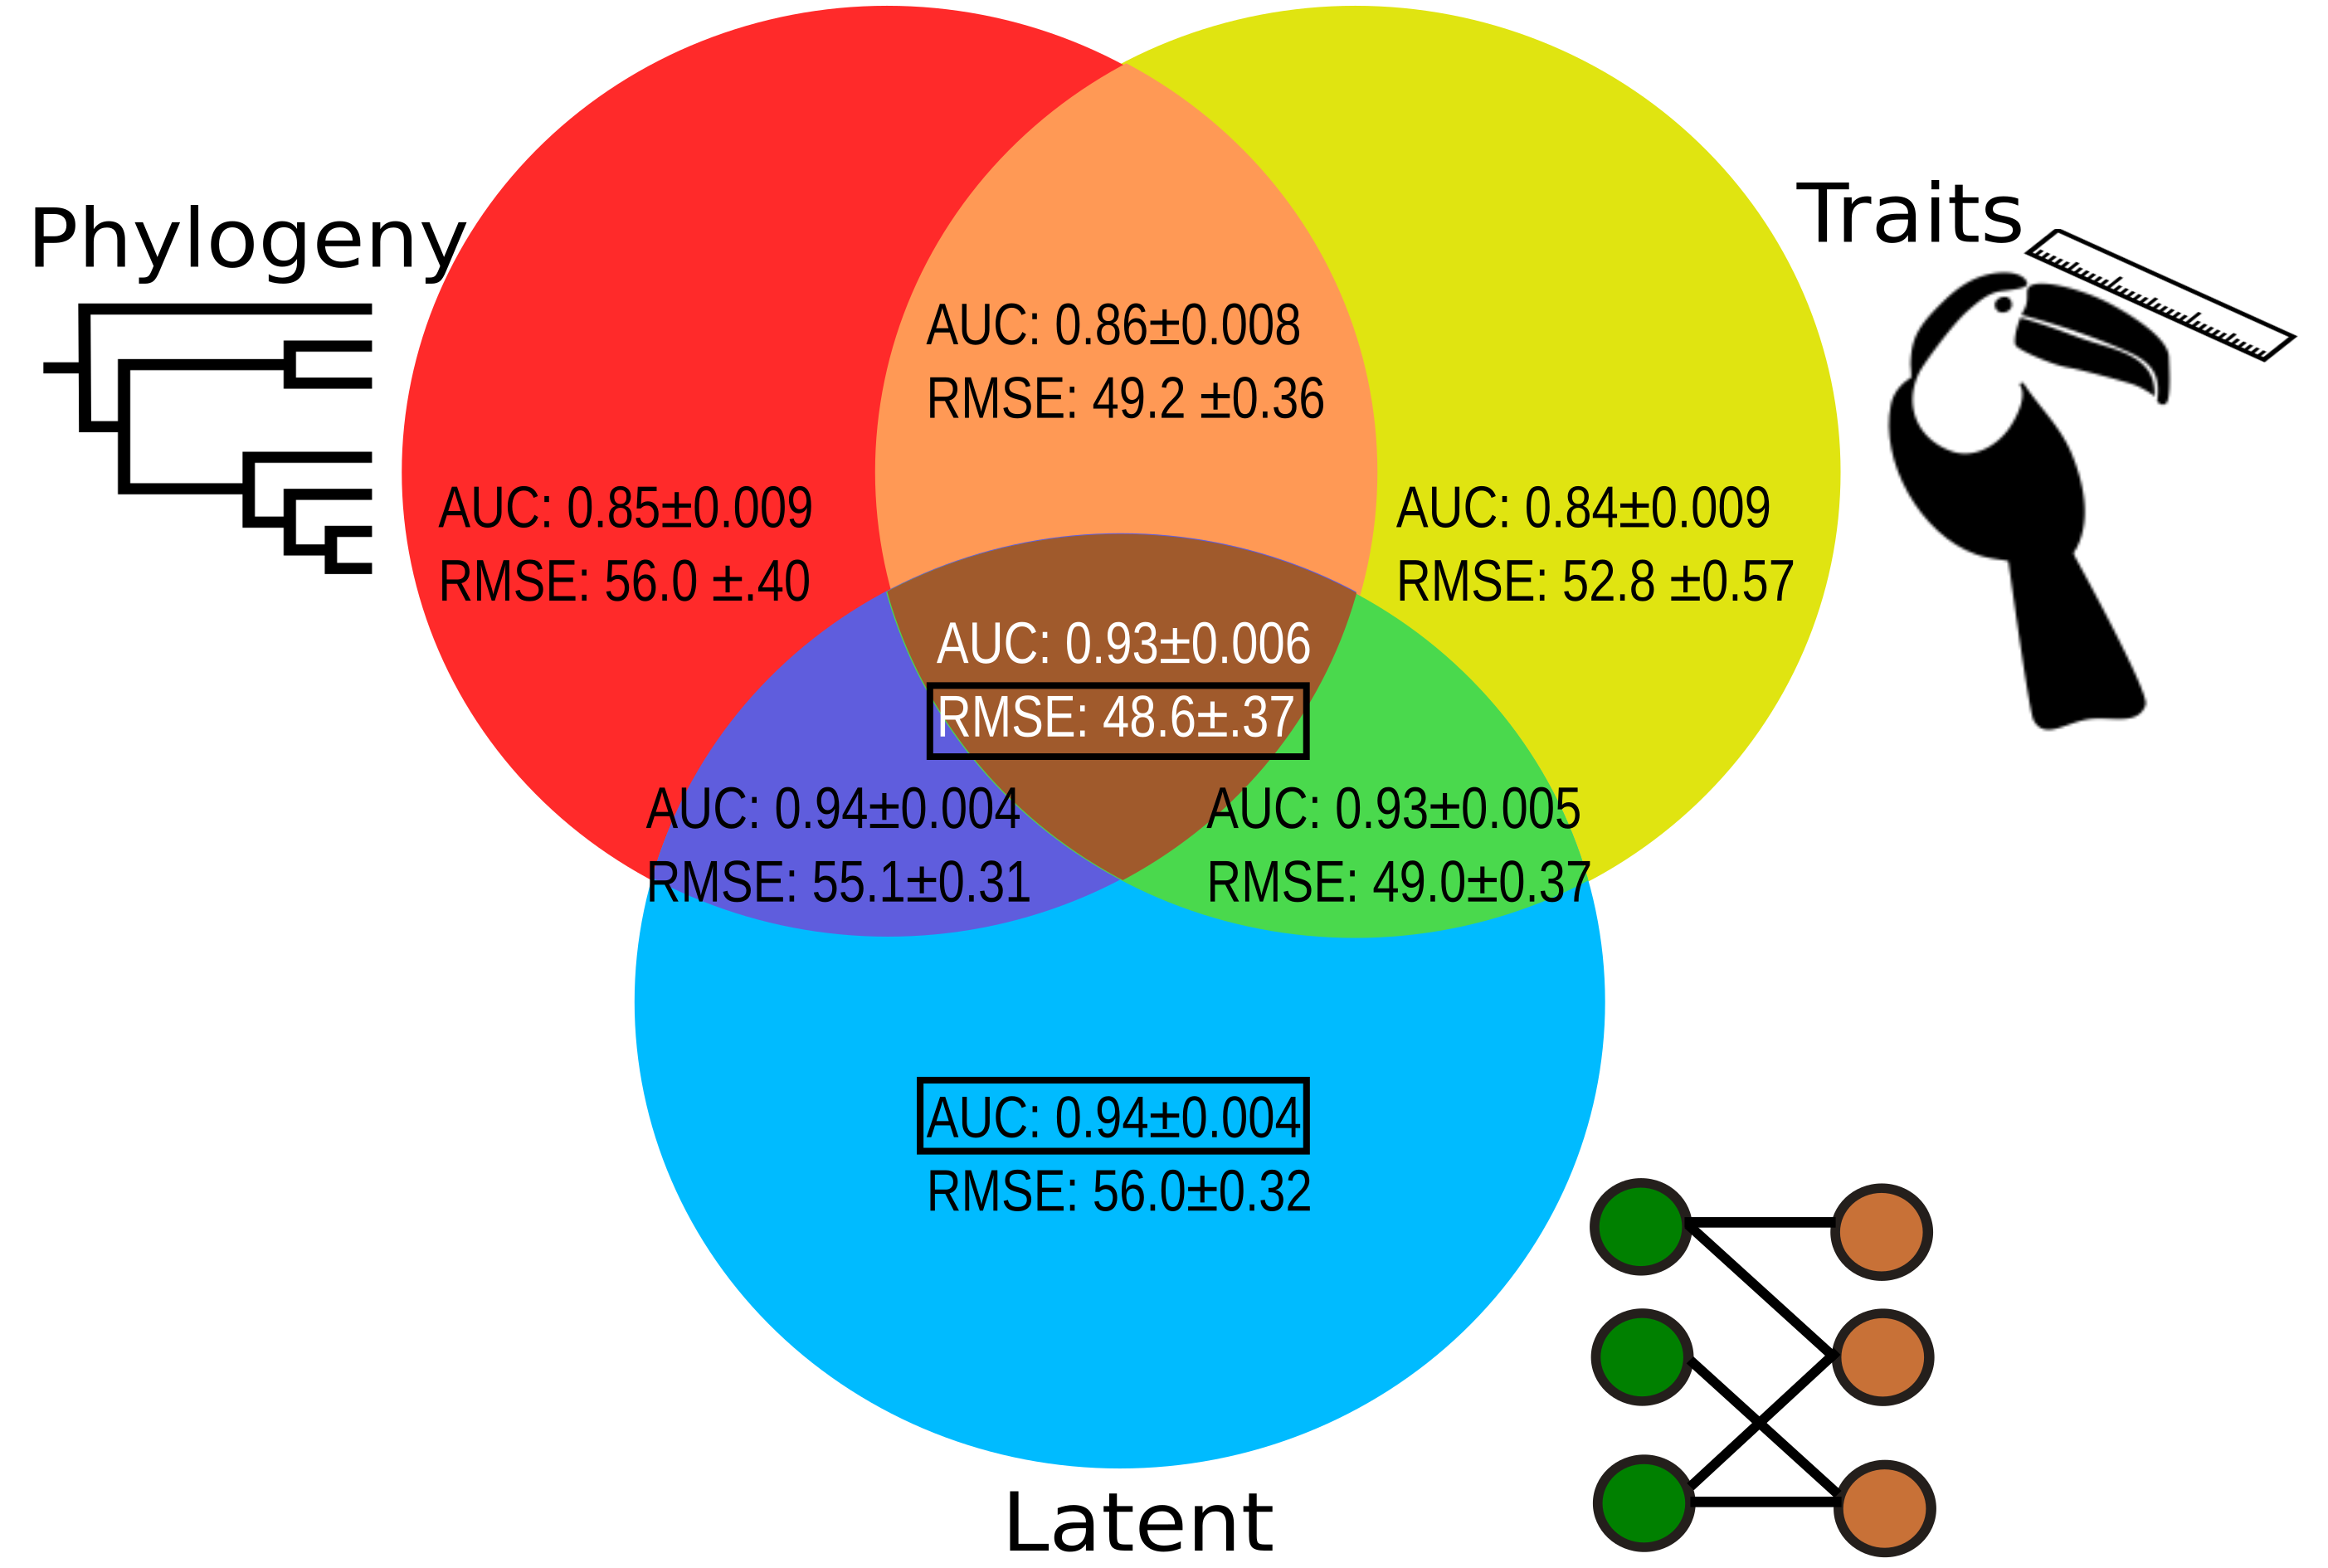
\includegraphics[width=\linewidth]{Fruglink/Figs/ReplicatePerformance_Polytomy.png}
\caption{Summary performance metrics of all 7 models, as measured by area under the receiver operating characteristic curve (AUC) and root mean squared error (RMSE); highest performing models for each metric are outlined in black. Mean metric values are presented from 100 replicates of each model structure alongside standard deviation. Model discriminatory power between links and non-links is maximized by including latent structural features, with the inclusion of trait, phylogenetic information, or both actually slightly decreasing discriminatory power. However, inclusion of trait and phylogenetic information, while not improving AUC, does increase overall model accuracy as measured by mean root squared error.}
\label{fig:Figure_1}
\end{figure}


\clearpage 

\begin{figure}%[tbhp]
\centering
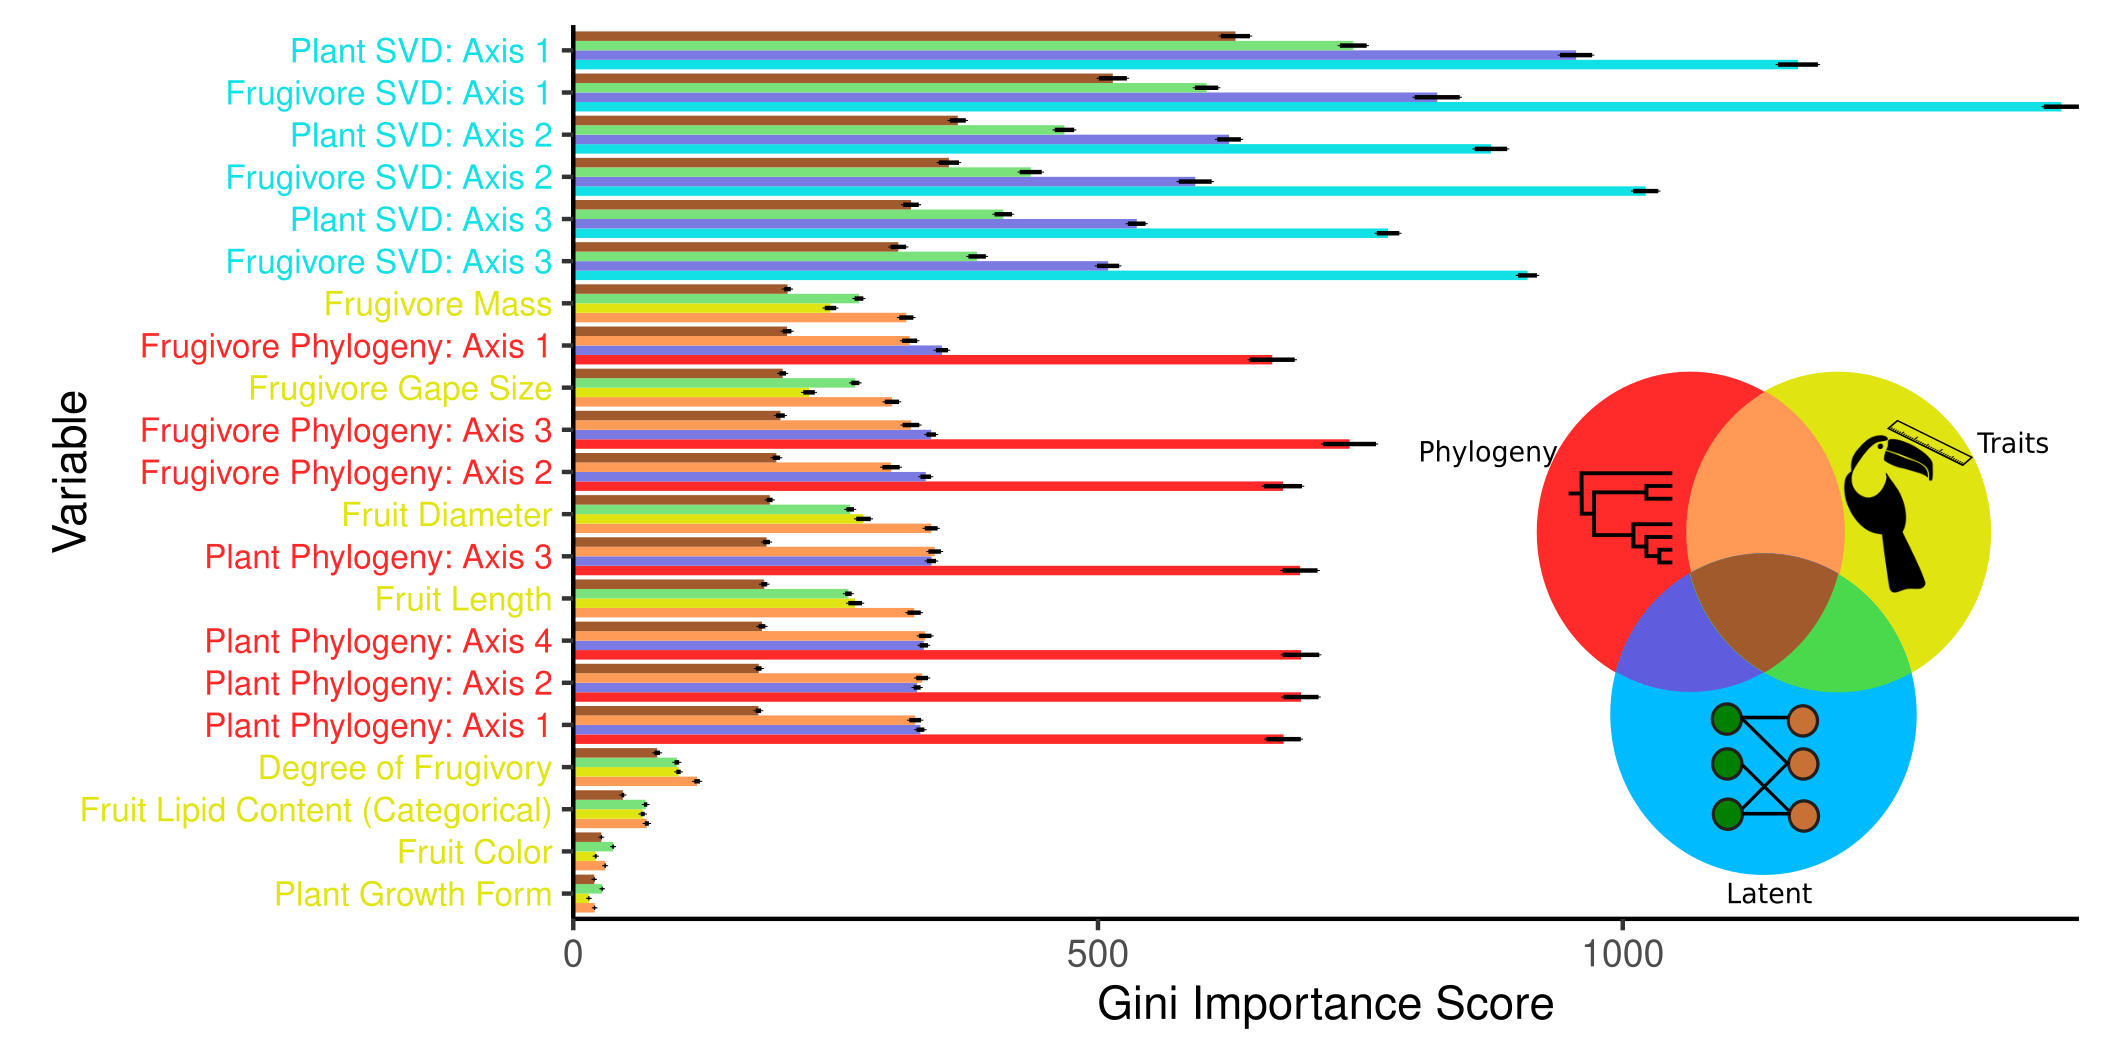
\includegraphics[width=\linewidth]{Fruglink/Figs/VarImportance_ErrBars_Short.png}
\caption{Variable importance across all models as measure by Gini importance score; color scheme is consistent with figure 1. In all models that include them, latent traits were consistently the most important variables for prediction. These were followed by continuous frugivore traits (body mass, gape size), and frugivore phylogenetic axes. Plant phylogenies and continuous trait information were generally less important for prediction than frugivore traits. Categorical plant traits (Lipid content, fruit color, growth form) were the least important variables for prediction.}
\label{fig:Figure_2}
\end{figure}



\clearpage 


\begin{figure}%[tbhp]
\centering
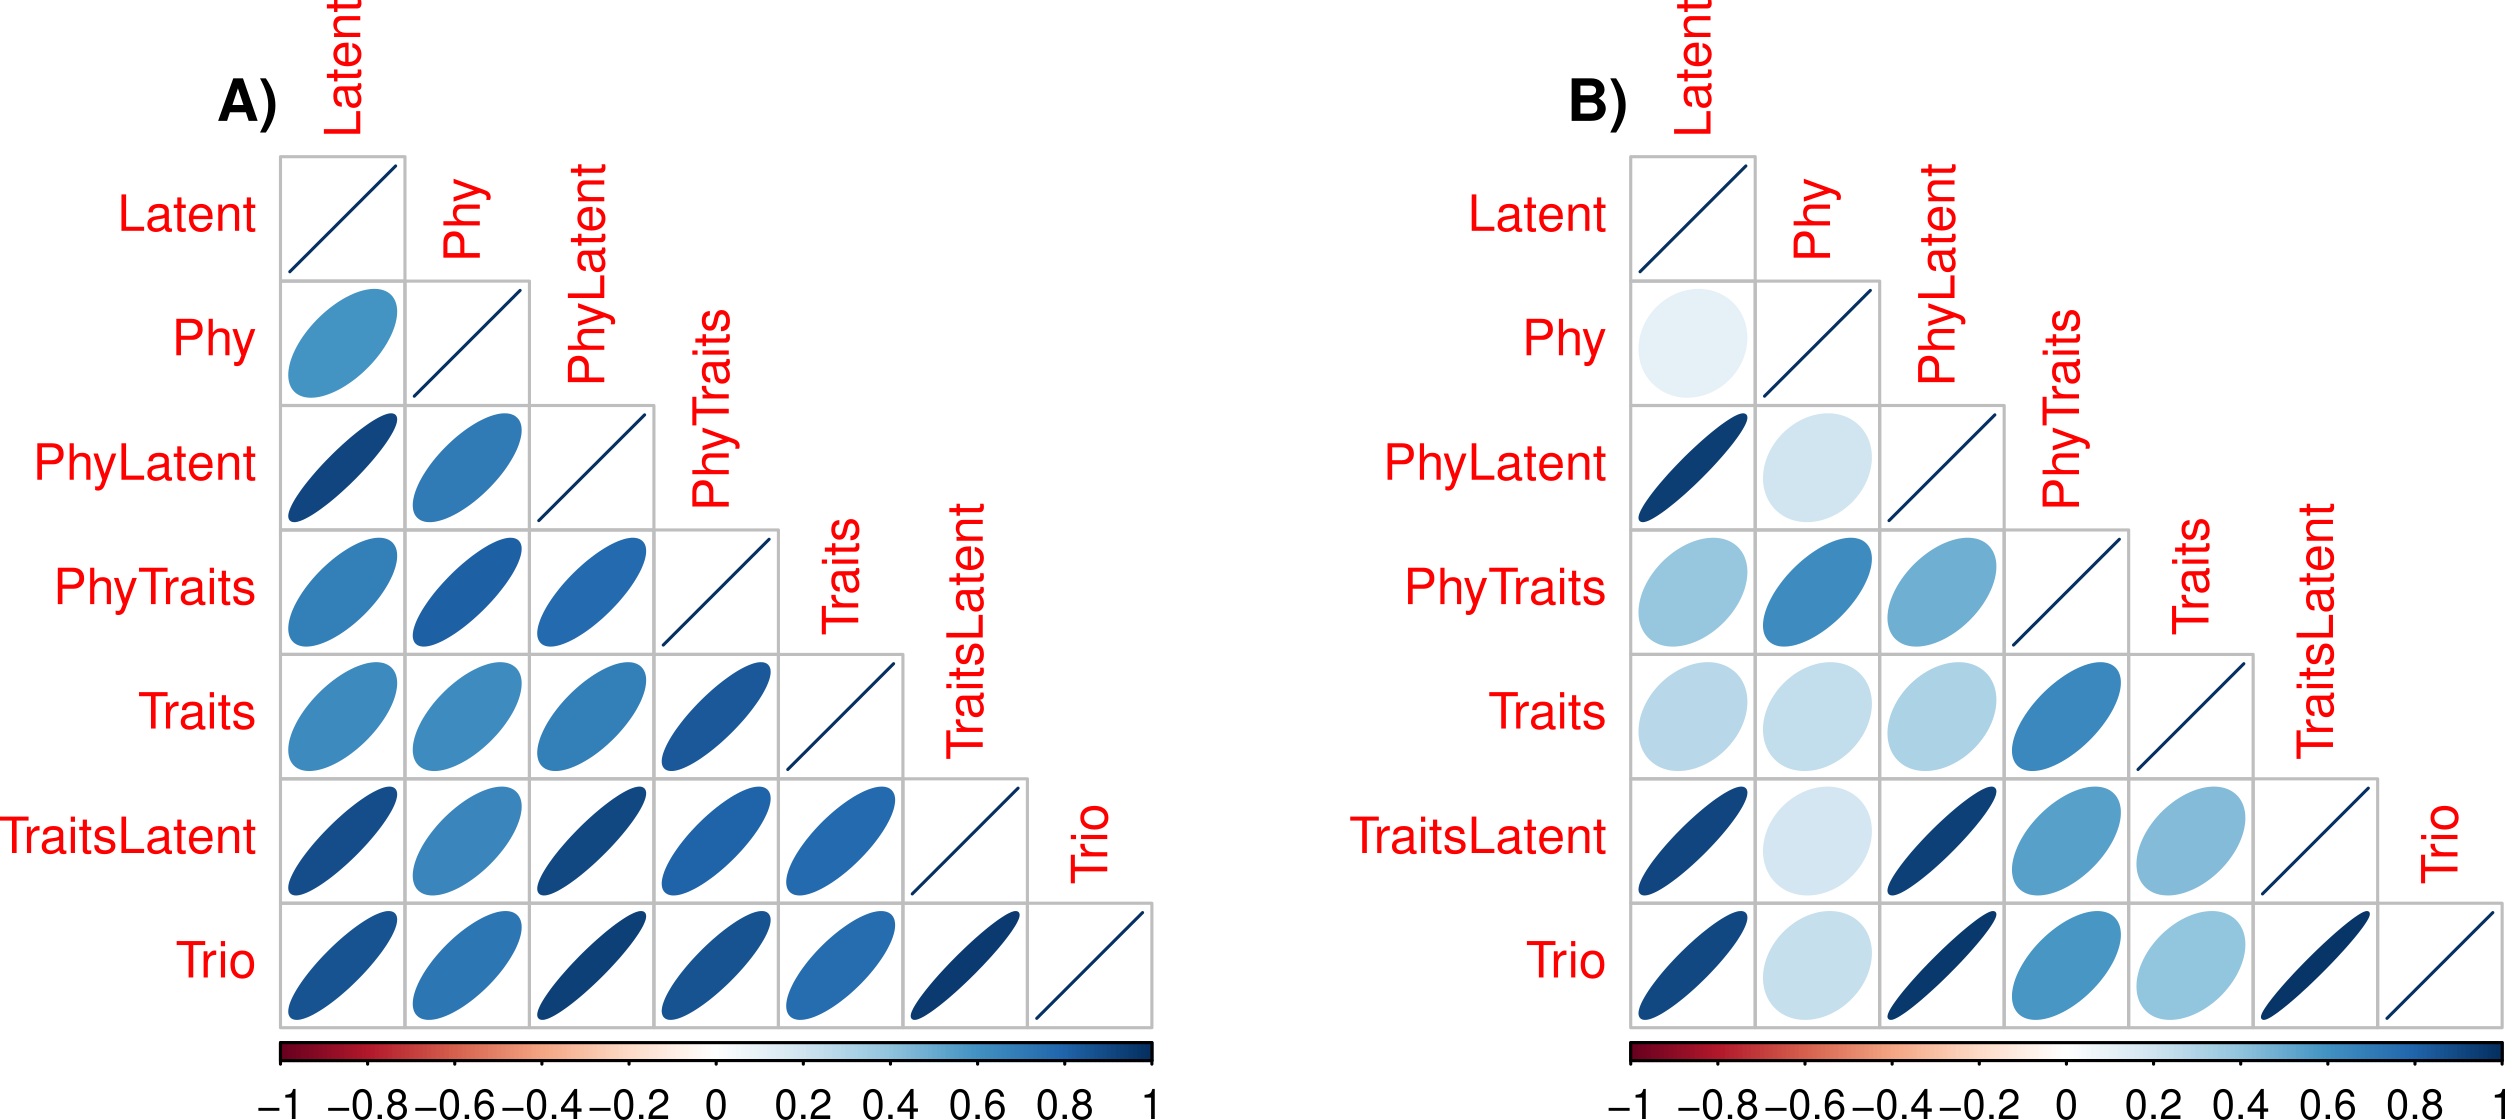
\includegraphics[width=\linewidth]{Fruglink/Figs/SpearmanCorplot_nolab.png}
\caption{Pairwise Spearman's rank correlations of link suitabilities across models for all potential interaction (A), as well as only unobserved interactions (B). The latter set of links represents both true forbidden links, as well as other potential interactions not observed in our data-set.}
\label{fig:Figure_3}
\end{figure}                             
                                                
                     
                          
\addtocontents{toc}{\protect\vskip-20pt}
\chapter[The impacts of geographic range size and niche breadth on species centrality in floral visitation networks]{The impacts of geographic range size and niche breadth on species centrality in floral visitation networks\footnote{In revision at \textit{Proceedings of the Royal Society: B}. Reproduced here under the CC BY 4.0 license terms. See Appendix D.}}   



\section*{\textbf{\underline{Abstract}}}
Understanding the factors that influence species' roles within ecological networks can provide insights into the rules governing the assembly of interaction networks. Centrality, a property describing how connected a given node is to the rest of a network, is often used to identify species whose loss may result in disproportionate effects on biotic communities. Understanding the drivers of species' centrality in floral visitation networks is crucial for understanding network responses to global change. Here, we test how geographic range size and niche breadth influence species centrality in floral visitation networks across spatial scales. We combine a globally distributed dataset of floral visitation networks comprising 30,330 interactions among 6,857 species with large-scale occurrence data to evaluate how species’ geographic and environmental range sizes impact their role in networks across scales. In global metawebs we observe a strong positive effect of geographic range size on closeness centrality, but that effect largely disappeared after accounting for spatial turnover in interactions. Instead, niche breadth showed a positive relationship with the standardized centrality of flowering plant species in both network types. Site-level centrality was tightly linked to species ranges. Together, these results emphasize the need for a multiscale perspective to understand the drivers and consequences of changes in ecological network properties across environments and scales.


\section*{\textbf{\underline{Introduction}}}

\paragraph*{}
Originating in mathematics, graph theory perspectives have become increasingly popular for the study of ecological networks throughout recent years \parencite{bascompte2007plant, landi2018complexity, valdovinos2019mutualistic, guimaraes2020structure}. Under this framework, interacting species can be represented as a series of nodes connected by links (interactions). What constitutes an ``interaction" is variable, set by the context of the system, and may include predation events, infections \parencite{dallas2017predicting}, floral visits \parencite{Young21}, or any number of other biotic interactions. By quantifying the full set of links present in a given system, we have gained insights into the structural properties of species interaction networks that allow us to better predict their potential responses to change \parencite{gilarranz2017effects}. For example, foundational work has linked network properties such as nestedness (the tendency for species with few interactions to link to species with many other interactions) and modularity (the tendency for species to interact more within given groups or ``modules'' than between them) to features such as network stability in response to perturbations or species extinctions \parencite{okuyama2008network, thebault2010stability, suweis2013emergence}.




\paragraph*{}
%TS: Species Centrality in Empirical Networks is important, and people try to predict it
In addition to these network-level properties, we can also measure the contribution of an individual node to overall network structure considering node-level properties. One of the most commonly analyzed node-level properties is centrality: a suite of measures describing how connected a given node is to the rest of the network. Highly central species may represent keystone species in a network, and removal of these nodes is likely to have outsized impacts on their associated communities \parencite{traveset2017plant, maia2019plant, martins2024propagation}. Identifying the eco-evolutionary processes that give rise to highly central species in local and regional-scale interaction networks is essential for understanding how ecological networks are organized and how they may respond to disturbances \parencite{moulatlet2023species, martins2025determinants, zhang2025network}. Previous work has emphasized the importance of species traits \parencite{watts2016influence, lazaro2020linking, maia2019plant} and evolutionary history \parencite{Gonzales2015macroecology, burin2021macroevolutionary} on influencing both network and node-level properties. Investigating determinants of a species' role within floral-visitation networks (defined here as its position and the distribution of interactions relative to other members in a network, captured through node-level properties such as centrality), can provide insights into biological processes underpinning interaction network structure across scales. Understanding these drivers in the context of floral visitation networks, which are often characterized by interaction generalism \parencite{waser1996generalization,stanton2003interacting} and frequent facultative interactions \parencite{geib2012tracing}, is of particular conservation importance as global declines in pollinator abundance and diversity threaten to potentially reduce pollination services in many ecosystems \parencite{potts2010global, rodger2021widespread}. 


%TS: Geographic range size may be associated with species role in a network. 
\paragraph*{}
In addition to morphological characteristics and phylogenetic history, the size of a species' geographic range may also impact its role in pollination networks at both local and global scales \parencite{moulatlet2023species, dattilo2020species}. 
% TAD: what does "its" in the sentence above refer to? I see what you're doing with the transition, but it's pretty awk. 
% GF: Rewrote. Still has an "its", but hopefully more clear. 
As species ranges increase in size, so does the total number of potential interaction partners. As a consequence, in regional metawebs (the set of species interactions observed across multiple local webs \parencite{poisot2012dissimilarity}) wide-ranging species may increase in their total number of interactions as both potential partners and interactions turn over across space \parencite{fricke2020accelerating, martins2022global}. 
% TAD: so now we have 2 different flavors of metaweb, regional and global?
% GF: I'm hoping that I can use "regional" as a catch-all (to have a metaweb you have to choose an "region" [extent] to aggregate over. In our case that's the globe. 
This accumulation of interactions across area, parallel to the classical species-area relationship \parencite{burkle2012shifts,sugiura2012scale, galiana2018spatial, dallas2021species}, may thus induce positive associations between species range size and species centrality at regional or global scales.
% TAD: but people have done interaction scaling, so why just be like "similar to species-area relationships"? You don't even have to cite my shit here if you don't want to, but I've done it. 
% GF: Hm; I was trying to reference the interaction-scaling lit here but maybe made things weird with the species-area relationship comparison. The citations here are mostly 
Additionally, species with broad geographic ranges may also be more central in local networks if geographic range size is associated with demographic or functional traits that may allow for generalist interaction strategies or high local abundance \parencite{holt1997relationship, hurtado2024generalism, Moulatlet2025General}. This potential confounder makes it difficult to differentiate the potential reasons geographic range size may impact species roles in mutualistic networks. The development of null modeling approaches, in which many random permutations of network linkages are summarized into an observed distribution of potential network property values, has been instrumental in making meaningful comparisons across ecological networks of different size and connectance \parencite{dormann2017, guimaraes2020structure, bluthgen2024critical}. Here, we utilize a null modeling approach in order to tease apart the otherwise confounding effects of turnover and range size \textit{per se} on species centrality across scales. 



\paragraph*{}
% We can think of "range size" geographically or environmentally
Species' geographic range size is driven by a number of biogeographic factors, including evolutionary history \parencite{webb2000geographic, alzate2025evolutionary}, dispersal limitation \parencite{alzate2022understanding}, biotic interactions \parencite{pigot2013species,galiana2023climate}, and climatic constraints \parencite{hausharter2023niche}. As species increase in the geographic extent they occupy, they may geographically overlap with more potential partners, increasing their centrality. However, geographic range size might not be the strongest predictor of the number of potential partners. Instead, species that occur in more climatically diverse environments may co-occur with a larger set of potential partners \parencite{slatyer2013niche, batstone2018using}. Therefore, species with broad abiotic niche breadths may have higher centrality in the global metaweb as a function of greater niche overlap with potential partners. A positive relationship between niche breadth and local centrality may also be observed if climatic and interaction generalism are positively associated, a feature observed in some food web systems \parencite{slatyer2013niche}. Niche breadth and geographic range size are fundamentally linked, though the exact shape of the relationship is dependent on the geographic availability of environments across space \parencite{dallas2025linking}.



%TS: Centrality means different things at the local and regional scale
\paragraph*{}
Biologically, species centrality has a fundamentally different meaning in local networks and global metawebs, and understanding how centrality scales between these contexts is still an open question in network ecology. Most existing work investigating the determinants of species centrality within networks to date has focused on local scales (\parencite{maia2019plant}, but see \parencite{moulatlet2023species}), as here node centrality has clear links to network properties \parencite{gonzalez2010centrality, maia2019plant, cagua2019keystoneness}. Species that occur in many local networks and are highly central in many or all of them may also exhibit high centrality in regional or global metawebs ( \parencite{estrada2007characterization, martins2025determinants} though see \parencite{dallas2022parasite}). However, even species with low local centrality can achieve high centrality in the global metaweb if they exhibit high interaction turnover across a wide geographic area \parencite{carstensen2014beta, simanonok2014partitioning}. At a global level, these central species may appear as relative generalists with many potential partners. However, at local scales, the realized set of interactions of any given individual or population may be relatively narrow \parencite{bison2015upscaling, arroyo2023intraspecific}. As such, understanding how centrality scales from local to global scales helps us better understand how population-level interaction patterns may vary across mutualistic species' ranges. 




% thesis
\paragraph*{}
To address these questions, we quantified variation in species-level centrality relative to geographic and environmental range size across a global assemblage of avian-plant and insect-plant floral visitation networks. Specifically, we tested whether species with broader geographic ranges or environmental niches occupy more central positions within local networks or global metawebs. We predicted that centrality will increase with range size and niche breadth in both contexts (Figure \ref{fig:conceptCentralRange}). At the metaweb scale, we expected species with broad ranges to turnover in interactions across geographic or environmental space, allowing them to accumulate more interactions across sites. At the local scale, we predicted a similar positive relationship driven by the positive association between interaction generalism and climatic or habitat generalism. Finally, we investigated whether these relationships persist after using null-model approaches to account for the impact of species co-occurrence on potential centrality measures. If range size or niche breadth continues to be positively associated with centrality under null models that control for co-occurrence, it would suggest a fundamental link between geographic or climate distributions and factors determining species role within mutualistic networks. Together, our results suggest that the impacts of range size on species centrality in large-scale metawebs are primarily driven by interaction turnover and the scaling of interaction specificity from local to global networks. When variation in interaction turnover is incorporated, niche breadth exerts the strongest positive effect on plant centrality within global networks. Consequently, species with large geographic ranges may appear to be relatively generalist in global metawebs due to high interaction turnover, but local-scale interaction patterns may exhibit more nuanced and variable relationships with species range limits. 

%----------
\section*{\textbf{\underline{Methods}}}

\paragraph*{Data}\mbox{}\\ 
We queried floral visitation networks through the Web of Life dataset, resulting in 97 networks with a total of 30,330 unique interactions between 6,857 species. We combined these networks into two global metawebs: one describing avian-plant interactions and another describing insect-plant interactions. Most studies only characterized one of these types of interactions; for the three studies that reported both insect and avian floral visits, we divided the network as appropriate. The avian-plant metaweb is comprised of 2,033 unique species-level interactions between 605 plant and 120 bird species across 31 sites. The insect-plant metaweb is larger, consisting of 28,297 interactions between 1,960 plants and 4,182 insect species across 66 sites. While expert range maps are available for most birds and some well-studied plant taxa, the majority of species in our study do not have up-to-date expert species range estimates available. In order to investigate the role of range size in determining species-level network traits, we estimated species ranges from available occurrence points. 

\paragraph*{Estimating Geographic Range Size}\mbox{}\\ 
For each species, we queried global occurrence records from the Global Biotic Information Facility (GBIF) using the \textit{gbifdb} $R$ package. Occurrence points were first processed using the \textit{coordinateCleaner} package; points were removed if they were present only in the fossil record, occurred within 2 km of country centroids, were not terrestrial, or were marked as an ``introduced" individual. To avoid overestimating species range size through including spurious or transient records in GBIF, we used a quantiled minimum convex polygon (MCP) approach. Within each continent -- based on a 7 continent model (Asia, Europe, Africa, Oceania, North America, Antarctica, and South America) -- we created the smallest minimum convex polygon that contains the central 95\% of the occurrence points within each continent. Range polygons were not created for species-continent combinations with less than 10 occurrence points. Total species' geographic range size was calculated as the total terrestrial area occupied across all continents. The points included within these polygons were also used for the calculation of environmental range (below). 2,554 species within our network had insufficient occurrence data to create species ranges; leaving a total of 4,303 species within our analysis (110 birds, 2,126 insects, and 2,067 plants). 


\paragraph*{Estimating Niche Breadth}\mbox{}\\ 
For each occurrence point, we extracted 56 climatic values from WorldClim at a 2.5 arc-minute resolution \parencite{fick2017worldclim}. These values represent a number of climatic variables potentially important for limiting species' distributions, averaged across the years 1970-2000. As these variables represent a high-dimensional environmental space that is collinear in many aspects, we performed a principal component analysis in order to reduce the dimensionality of our niche space \parencite{kriticos2014extending, dallas2025linking}. The first two principal components of this climatic space explain over 77\% of the total climatic variation. For each species, we plotted each occurrence point that fell within the 95\% quantiled geographic range polygon calculated above onto the Cartesian plane defined by these two PCA axes, combining points from all continents on which a species occurred. We then again employed a minimum convex polygon approach to draw an environmental range in this PCA space for each species (i.e., its niche breadth).

\paragraph*{Centrality Measures}\mbox{}\\ 
Insect and avian floral visitor metawebs contained 6142 and 725 total species, respectively. The vast majority of species in each network were connected to one major component (the largest set of interconnected nodes). As centrality measures become non-comparable in unconnected graphs, we dropped species that were not part of these major components. This resulted in the removal of 51 (0.83\%) and 4 (0.55\%) species from the insect and avian metawebs, respectively. Closeness centrality (which describes the mean proximity of one node to all other reachable nodes within the network, Figure \ref{fig:conceptCentralRange}) was calculated for nodes in the remaining simply connected networks using the \textit{igraph} package. 
% TAD: why give a weirdly technical def of closeness? It's not wrong or bad, but you want plant-frugivore folks reading this. It's proportional to the mean proximity of one node to all other reachable nodes in the network. GF: Casual-ified! 
We chose closeness centrality as an intermediate between hyper-local measures of centrality (e.g., degree centrality) and hyper-global measures (e.g., eigenvalue centrality). At the global metaweb scale, the rank of alternative measures of centrality were positively correlated, though to varying degrees (Figure \ref{fig:S2}).

\paragraph*{Null model expectations of species centrality}\mbox{}\\ 
While centrality measures are designed to be comparable between nodes of the same network, their absolute value is heavily influenced by network size and connectance, potentially hindering comparisons across networks. To address this when measuring species-level centrality in local networks, we used a null-model approach to standardize centrality within each local network. For each local network, we first measured the closeness centrality of all component species species using a similar approach to the global metaweb.
% TAD: you use lots of possessives (e.g., 'its') and it makes it read weird. If that's just your style, stick to it, but I am not a fan. 
%GF: Took out a couple of the most confusing ones; hopefully the remaining ones are relatively clear. 
We then used the \texttt{vegan} package to generate 1000 randomized versions of each local network by permuting interaction links while preserving each node's degree (effectively preserving marginal totals of the interaction matrix). This allowed us to characterize the potential distribution of centrality values for each node, given that node's degree and the network's overall structure. We then $z$-transformed the observed centrality values using the mean and standard deviation of this null distribution to create a $z-$transformed measure of local closeness centrality for each species-site combination. 


\paragraph{} To extend this approach to the metaweb level, we pooled permuted local webs to construct null global metawebs. This allowed us to generate a null distribution of species-level closeness centrality across the entire metaweb, accounting for each species' presence across multiple local networks. Observed metaweb centrality values were then $z-$transformed relative to this distribution. We investigated both measured and $z-$transformed centrality at the metaweb scale. At the local scale we only modeled $z-$transformed centrality, as raw measures of centrality are not directly comparable across differently sized networks. One insect-plant and three avian-plant networks were too small to create realistic null distributions, and were subsequently excluded for local centrality analyses. 


\paragraph*{Statistical Analyses}\mbox{}\\ 
We examined the role of species range size and niche breadth on species centrality through Bayesian generalized linear models implemented in Stan \parencite{carpenter2017stan} through the $R$ package \textit{brms} \parencite{burkner2017brms}. In order to facilitate comparison and meaningful interpretation of interaction effects, both geographic range sizes and niche breadth values were log-transformed and then rescaled to a mean of 0 and standard deviation of 1. All models therefore shared the generalized form of predicting a given species' centrality as a function of geographic range size, niche breadth, and the interaction between these predictors. Niche breadth or geographic range size may exert fundamentally different effects on the centrality of flowering plant species compared to floral visitors. As such, we analyze node types (floral visitor or flowering plant) separately for each network or set of networks, effectively repeating our modeling approach for all factorial combinations of: scale (metaweb vs local webs), network type (insect-plant vs avian-plant), and interactor type (floral visitor vs flowering plant). Accounting for our two alternative centrality measures at the metaweb scale (measured and $z-$transformed closeness centrality), this resulted in 12 models total. We use vague priors centered on 0 for all slope and intercept coefficients. All models were fit using 5 Markov chain Monte-Carlo simulations, each with 5,000 iterations following a 1,000 iteration burn-in period; posterior samples were sampled without thinning \parencite{link2012thinning}. Simulation convergence was checked through visual inspection of traceplots. Gelman-Rubin statistics fell below 1.01 for all parameters across all models.  For slope terms we sampled the resultant posterior distributions and approximated the two-sided posterior probability ($POP_2$) as twice the proportion of posterior samples falling above or below 0 (whichever is smallest), a Bayesian analog to traditional frequentist p-values \parencite{shi2021reconnecting}. Relationships between fit slope values across models are presented as pairs plots in supplemental figures \ref{fig:S6}-\ref{fig:S11}. 

\paragraph{}
For the subset of species which occurred across multiple sites, we further investigated the role interaction turnover may play in determining species centrality in global metawebs. As both the degree of turnover and number of sites at which a species occurs may have nonlinear effects on metaweb centrality, we investigate these factors through a generalized additive modeling (GAM) approach. For each node the that occurred in multiple sites (1,166 species), we calculated the Simpson's dissimilarity of interaction partner sets across all sites in which they occurred \parencite{baselga2015comparing}, as implemented in the $R$ package \texttt{betapart} \parencite{baselga2012betapart}. We created GAM models predicting metaweb centrality (either raw values or $z-$transformed, scaled to a mean of 0 and standard deviation of 1 to facilitate comparisons across models) as a function of the tensor product of interaction turnover and number of local sites. We investigate the $p-$value of tensor terms, as well as compare estimated degrees of freedom to maximum allowable degrees of freedom ($k'$) as well as visually inspected model residuals to assess model fit. %Plots illustrating the resultant partial effects of turnover across are show in Figure \ref{fig:gam}. 

% TAD: have you defined k'? might be worth just spelling it out instead of the notation. You want the reader to follow, and you've already been talking about tensor products. 
% GF: Definition added


% -------------------
\section*{\textbf{\underline{Results}}}

\paragraph*{Species Occurrences and Interactions}\mbox{}\\ 
Species' geographic range sizes in insect-plant networks varied widely, ranging from 2,232 km$^2$ (\textit{Chaetanthera lycopodioides}, a range-restricted montane Aster endemic to Chile and Argentina \cite{arroyo2007display}) to over 119 million km$^2$ (\textit{Sonchus oleraceus}, a cosmopolitan weed native to Eurasia), with a median value of 3,749,391 km$^2$. Geographic distributions of species in avian-plant visitation networks ranged from 2,518 km$^2$ (\textit{Barbacenia longiflora}, a monocot forb restricted to Minas Gerais, Brazil) to over 85 million km$^2$ (\textit{Prunella vulgaris}, a cosmopolitan invasive weed), with a median value of 1,536,647 km$^2$. Across sites, geographic and environmental range size were positively correlated ($r$=0.667, $p <$ 0.001). Typical of large-scale interaction metawebs, realized connectance (the percentage of realized links out of the total possible number of interactions) was low \parencite{jordano1987patterns}. At the global scale, only 0.32\% and 2.8\% of potential links were realized in insect and avian interaction metawebs, respectively. At the site-level, average connectance of insect-plant networks was 0.194, whereas average avian-plant network was 0.356. 

% TAD: numbers don't go in math font unless you're willing to put every number in math font. 
%GF: Fixed

%TD: what the fuck is POP_2? 
%GF: I put the explanation of this at the very end of the methods, but it is a weird metric. It just seemed like a better for shorthand for "our 95% Credible Interval does or doesn't overlap 0" as well as being a closer analog to like hypothesis testing. But keeping it isn't a make or break for me. 
% TD: eh. Give it a cooler name? \omega_{95}? Idk man. 


%Effect in metaweb
\paragraph*{Global Metawebs}\mbox{}\\ 
At the metaweb scale, geographic range size was positively associated with species centrality of all node types across both insect and avian networks (Figure \ref{fig:MetawebEffect}). However, once accounting for potential co-occurrence through $z$-transformation, geographic range size showed no association with metaweb centrality for avian or insect floral visitors, or insect-visited plant species, and instead showed a negative association with the centrality of avian-visited plant species ($POP_2=$0.020). Niche breadth had a negative impact on centrality for plants and insects within the insect-plant metaweb after controlling for geographic range size ($POP_2<$0.001, $POP_2=$0.028). After $z$-transformation, niche breadth instead had a positive impact only on plant centrality in both insect and avian metawebs ($POP_2<$0.001 across both networks) while showing no effect for floral visitors. There was no significant interaction effect between geographic range size and niche breadth on unstandardized metaweb centrality across node types. However, after $z$-transformation, plants in both network types showed positive interaction effects ($POP_2<$0.001 and $POP_2=0.009$ for insect and bird-visited plants, respectively).



\paragraph{} For species that occurred across multiple sites, interaction turnover varied from 0 (complete conservation or nestedness of interactions across sites) to 1 (no overlap in interactions across sites), with a mean value of 0.644. The tensor product of interaction turnover and number of sites was statistically significant in predicting both raw and $z-$transformed metaweb centrality ($p<0.001$), but varied widely in the amount of variance explained. For the GAM model predicting measured metaweb centrality $R^2=0.231$, with interaction turnover exhibiting a positive partial effect across much of the realized parameter space, particularly for species with the highest centrality values (Figure \ref{fig:gam}). After $z$-transformation, the tensor product of turnover and number of sites still exhibited a statistically significant effect ($p<0.001$) but explained little of the overall variation ($R^2=0.054$). Taken together these results further suggest that positive relationships between species' geographic range size and measured metaweb centrality are largely driven by interaction turnover across sites. 



%Effect on local webs
\paragraph*{Local Webs}\mbox{}\\ 
Average species centrality in local floral visitation networks was positively correlated with their centrality in their respective global metawebs ($r=0.480$ and $p<0.001$ for insect webs, while $r=0.079$ and $p=0.035$ for avian webs). Species that occurred at multiple sites showed variable centrality across their respective local webs (Figure \ref{fig:S3}). Geographic range size was negatively related to the local centrality of insect-visited plant species (Figure \ref{fig:LocalPlot}, $POP_2=$0.018). Conversely, niche breadth was positively related to the average local centrality of nodes within insect networks ($POP_2<$0.001 for plants, $POP_2=$0.004 for insects). Insect-visited plants also exhibited a positive interaction term between geographic range size and niche breadth on average local centrality ($POP_2=$0.022). We failed to find any significant effect of range size, niche breadth, or their interaction on the local centrality of species within avian networks.






\section*{\textbf{\underline{Discussion}}}
%The effect of geographic range size on metaweb centrality is mediated through cooccurrence. 
\paragraph*{} Generally we find species' geographic range size and niche breadth are more clearly linked to their centrality in aggregate plant-pollinator metawebs than within local interaction networks. The positive impact of geographic range size on metaweb centrality we observed across all node classes may be caused by a number of potential drivers. Species with broad geographic ranges are likely to co-occur with more potential interaction partners across their range (Figure \ref{fig:S4}). In this case, even if species are relatively peripheral across local networks, they may be relatively central at the metaweb level if interaction turnover is high across their range \parencite{martins2025determinants}. Our results support this interpretation, as while species with large geographic ranges tended to be more central in the global metaweb, they did not tend to be more central than null expectations based on their connections across all local webs (Figure \ref{fig:MetawebEffect}). Additionally, generalized additive models indicated a large partial effect of interaction turnover on measured metaweb centrality, but this affect largely disappeared once these centrality values were $z-$transformed (Figure \ref{fig:gam}). Together, these patterns suggest that, at the global scale, species centrality in these metawebs is shaped more by neutral processes-namely the accumulation of interactions across space-than by the specific identity of those interactions. 

\paragraph*{}
Contrary to our expectations, standardized centrality was negatively related to geographic range size of plants in avian-plant networks after accounting for niche breadth. This pattern may indicate slower accumulation of interactions across space (lower interaction turnover) than otherwise expected. This pattern may be driven by wide-ranging, disturbance-adapted species that occur in many networks but are less likely to form interactions with narrowly distributed specialists. Nectarivory has evolved numerous times within birds, but contemporary biogeographical distributions of avian nectarivore diversity is clustered in the neotropics and parts of Australasia \parencite{kissling2012bird}. This spatial clustering of potential partner diversity may drive lower rates of interaction turnover of avian-pollinated plants across large spatial scales. 

%The effect of environmental range size only impacts plants (mostly when $z-$transformed). 
\paragraph*{}
After $z$-transformation, metaweb centrality was positively related to niche breadth in plants of both metawebs, but was unrelated in floral visitors. If plant species are limited in their dispersal by the availability of mutualists \parencite{warren2014mutualism, duffy2017specialized}, species with broad ranges of potential partners may be able to exploit a more climatically diverse set of environments. The availability or efficacy of mutualists may increase the abiotic tolerances of some species \parencite{warren2014mutualism, fowler2023geographic}, effectively expanding their climatic niche breadth. Batstone et al. (2018) outline how environmental variability may favor interaction generalism by altering the availability or efficacy of mutualists \parencite{batstone2018using}. Similar mechanisms may occur across an organism's range; plants with climatically diverse ranges may experience parallel changes in partner availability or efficacy, promoting interaction generalism \parencite{hurtado2024generalism}. Alternatively, in systems characterized by widespread generalism, plant species with broad niche breadths may participate in more interactions as they co-occur with a broader complement of potential pollinators. Understanding the mechanisms of this interplay between a species' climatic niche breadth and its position within local and global networks warrants further study. 

\paragraph*{}
In contrast to global metawebs, both geographic range and niche breadth show a reduced effect on species centrality at the local scale. In insect networks, average local centrality was positively related to niche breadth across both node types, but negatively related to geographic range size in insect-visited plant species. We also detected a positive interaction between range size and niche breadth on the centrality of plant species in insect-floral visitation networks, indicating that their combined influence shapes local structure of these networks (Figure \ref{fig:LocalPlot}). Species with broad geographic ranges tended to be more central when they also had broader climatic niches, whereas species with narrow ranges were more central when they exhibited broader niche breadths. This suggests multiple ecological pathways or strategies that may result in high centrality in local networks. Widely distributed species with broad abiotic tolerances may be relatively generalized in their interaction patterns at local scales, increasing centrality \parencite{hurtado2024generalism}. Alternatively, narrowly distributed climatic specialists may also be highly central, potentially through achieving high abundance in restricted environments \parencite{suarez2023dispersal}. The functional consequences of a species' centrality within a network may vary greatly across local, regional, and global scales, and further investigation of how centrality scales across levels of organization is of great interest. In our study, networks are either analyzed at the site level, or aggregated into global metawebs. Fully understanding the processes of scaling from local to global requires hierarchical sampling designs replicated across large geographic extents. While understanding the scaling of network properties across space, environments, and time has received a great amount of conceptual attention in recent years \parencite{tylianakis2008global,morales2008effect, burkle2011future,  moulatlet2023species}, the logistical challenges of research across these scales has limited our ability to fully explore these questions in some cases. 

\paragraph*{}
The emergent consequences of a species' centrality may ultimately differ across local to global scales. For example, at local scales the perturbation of highly central species may propagate farther or more strongly through a mutualistic community than the same perturbation applied to more peripheral species \parencite{Cauga2019, delmas2019, martins2024propagation}. Across larger scales, highly central species may play key roles in allowing mutualistic metacommunities to persist \parencite{filotas2010effect}, especially in the face of habitat heterogeneity or disturbance \parencite{prakash2004habitat}. Patterns of interaction turnover across space are closely linked to both the causes and consequences of centrality scaling relationships. While the temporal turnover of mutualistic interactions is fairly well appreciated in phenological contexts \parencite{olesen2008temporal, chavez2020drivers}, empirical patterns of interaction turnover across space, habitats, and environments warrant further study \parencite{tylianakis2017}. 


\paragraph*{}
Understanding the factors that determine species positions in mutualistic networks across scales is a fundamental question in network ecology. Our study identifies geographic range size as a key determinant of species centrality in floral visitation metawebs, largely driven by the spatial accumulation of interactions across sites. At the local scale, we also find that climatic niche breadth interacts with geographic range size to predict plant centrality in insect-plant networks, highlighting the multiple pathways through species may become highly central at the site level. Together, these results emphasize the need for a multiscale perspective to understand the drivers and consequences of changes in ecological network properties across environments. 
\\

\noindent \textbf{Data accessibility}: Data and $R$ code necessary to recreate this analysis is available on on figshare at \url{https://figshare.com/s/ab0b46493fd69cf4a2c8}\\

\section*{\textbf{\underline{Figures}}}

\begin{figure}[H]
    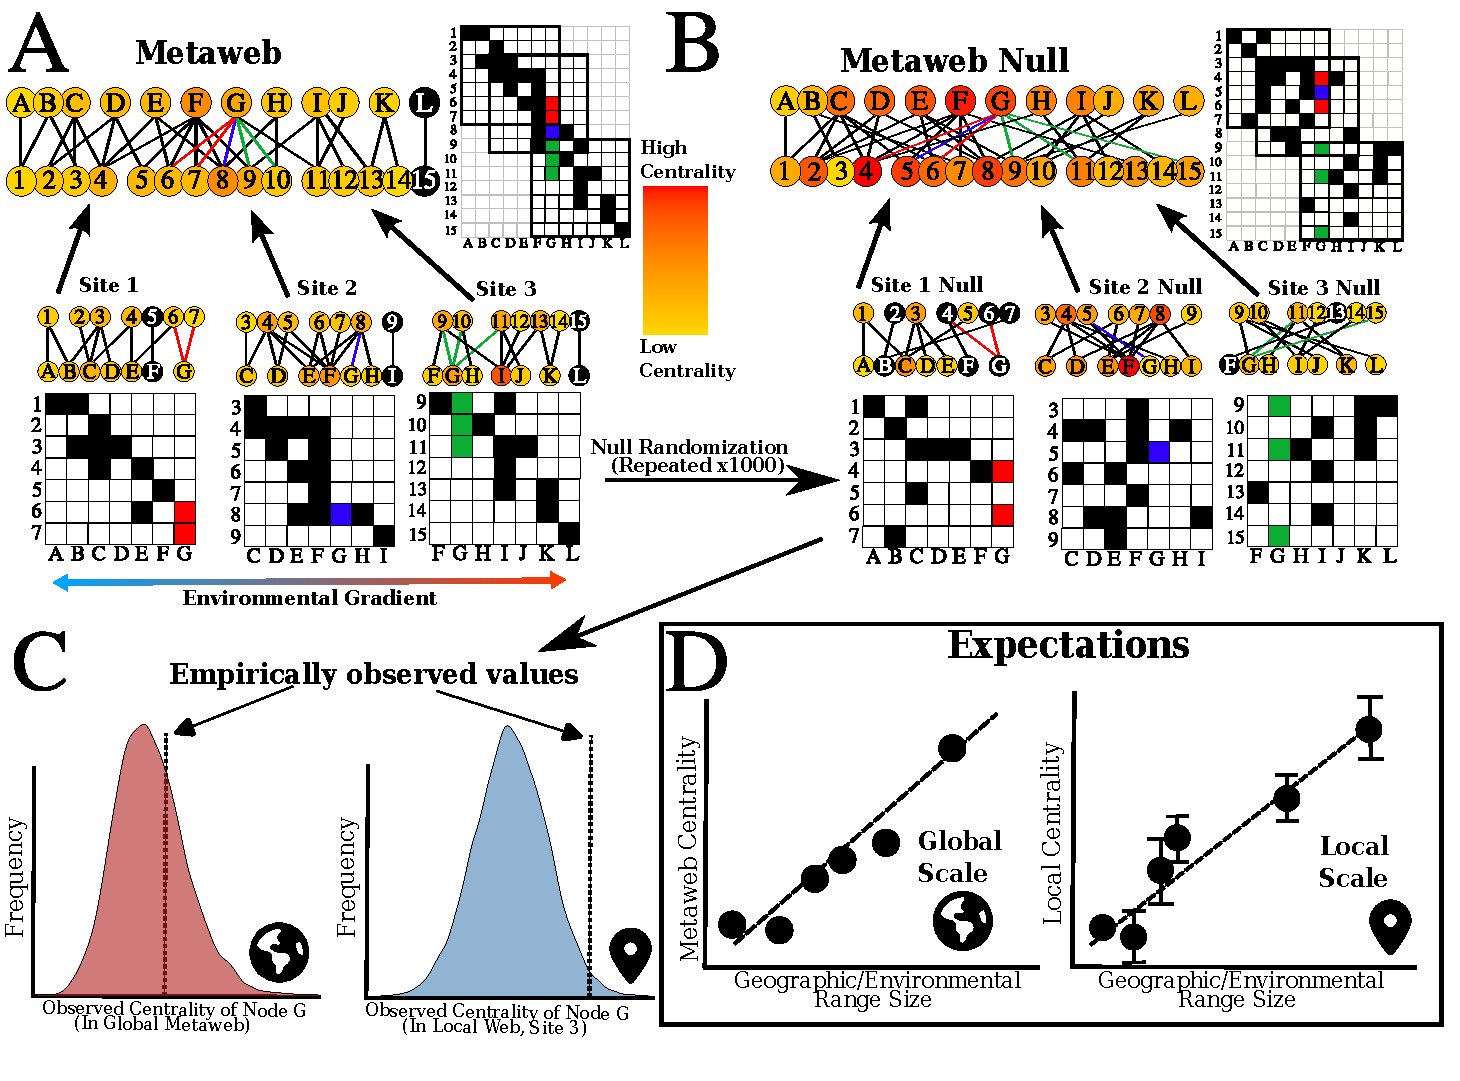
\includegraphics[width=22cm, angle=90, alt={Theoretical diagram summarizing the effects of geographic range size and niche breadth and network centrality across geographic scales}]{centralRange/figs/pdf/Concept_v2_busy_sized.pdf}
    \label{fig:conceptCentralRange}
\end{figure}

\addtocounter{figure}{0}
\begin{figure} [H]
  \caption[Geographic range size and node centrality]{Local interaction networks are embedded along natural environmental gradients (A), with species occurring in one or more sites and contributing interactions to a global metaweb, defined as the union of all observed interactions across sites. At the metaweb scale, species with broad geographic ranges or wide abiotic tolerances may accumulate interactions across multiple sites. At the local scale, such species may also be more central if interaction generalism covaries with environmental or habitat generalism. Species centrality can be quantified within individual site-level networks as well as in the global metaweb (node color). However, metaweb centrality is jointly influenced by the identity of interactions and by interaction turnover across sites. To isolate these effects, we implement a site-level null randomization (B) that shuffles interaction identities within each site while preserving the total number of interactions per species. Repeating this procedure generates null distributions of expected centrality values for each species at both local and metaweb scales (C), given the constraints of observed local network structure. Empirical centrality values can then be standardized (e.g., $z-$transformed) relative to these expectations, allowing scale-dependent effects of range size on network centrality to be evaluated (D).}
\end{figure}

\clearpage 




\begin{figure}[H]
\centering
    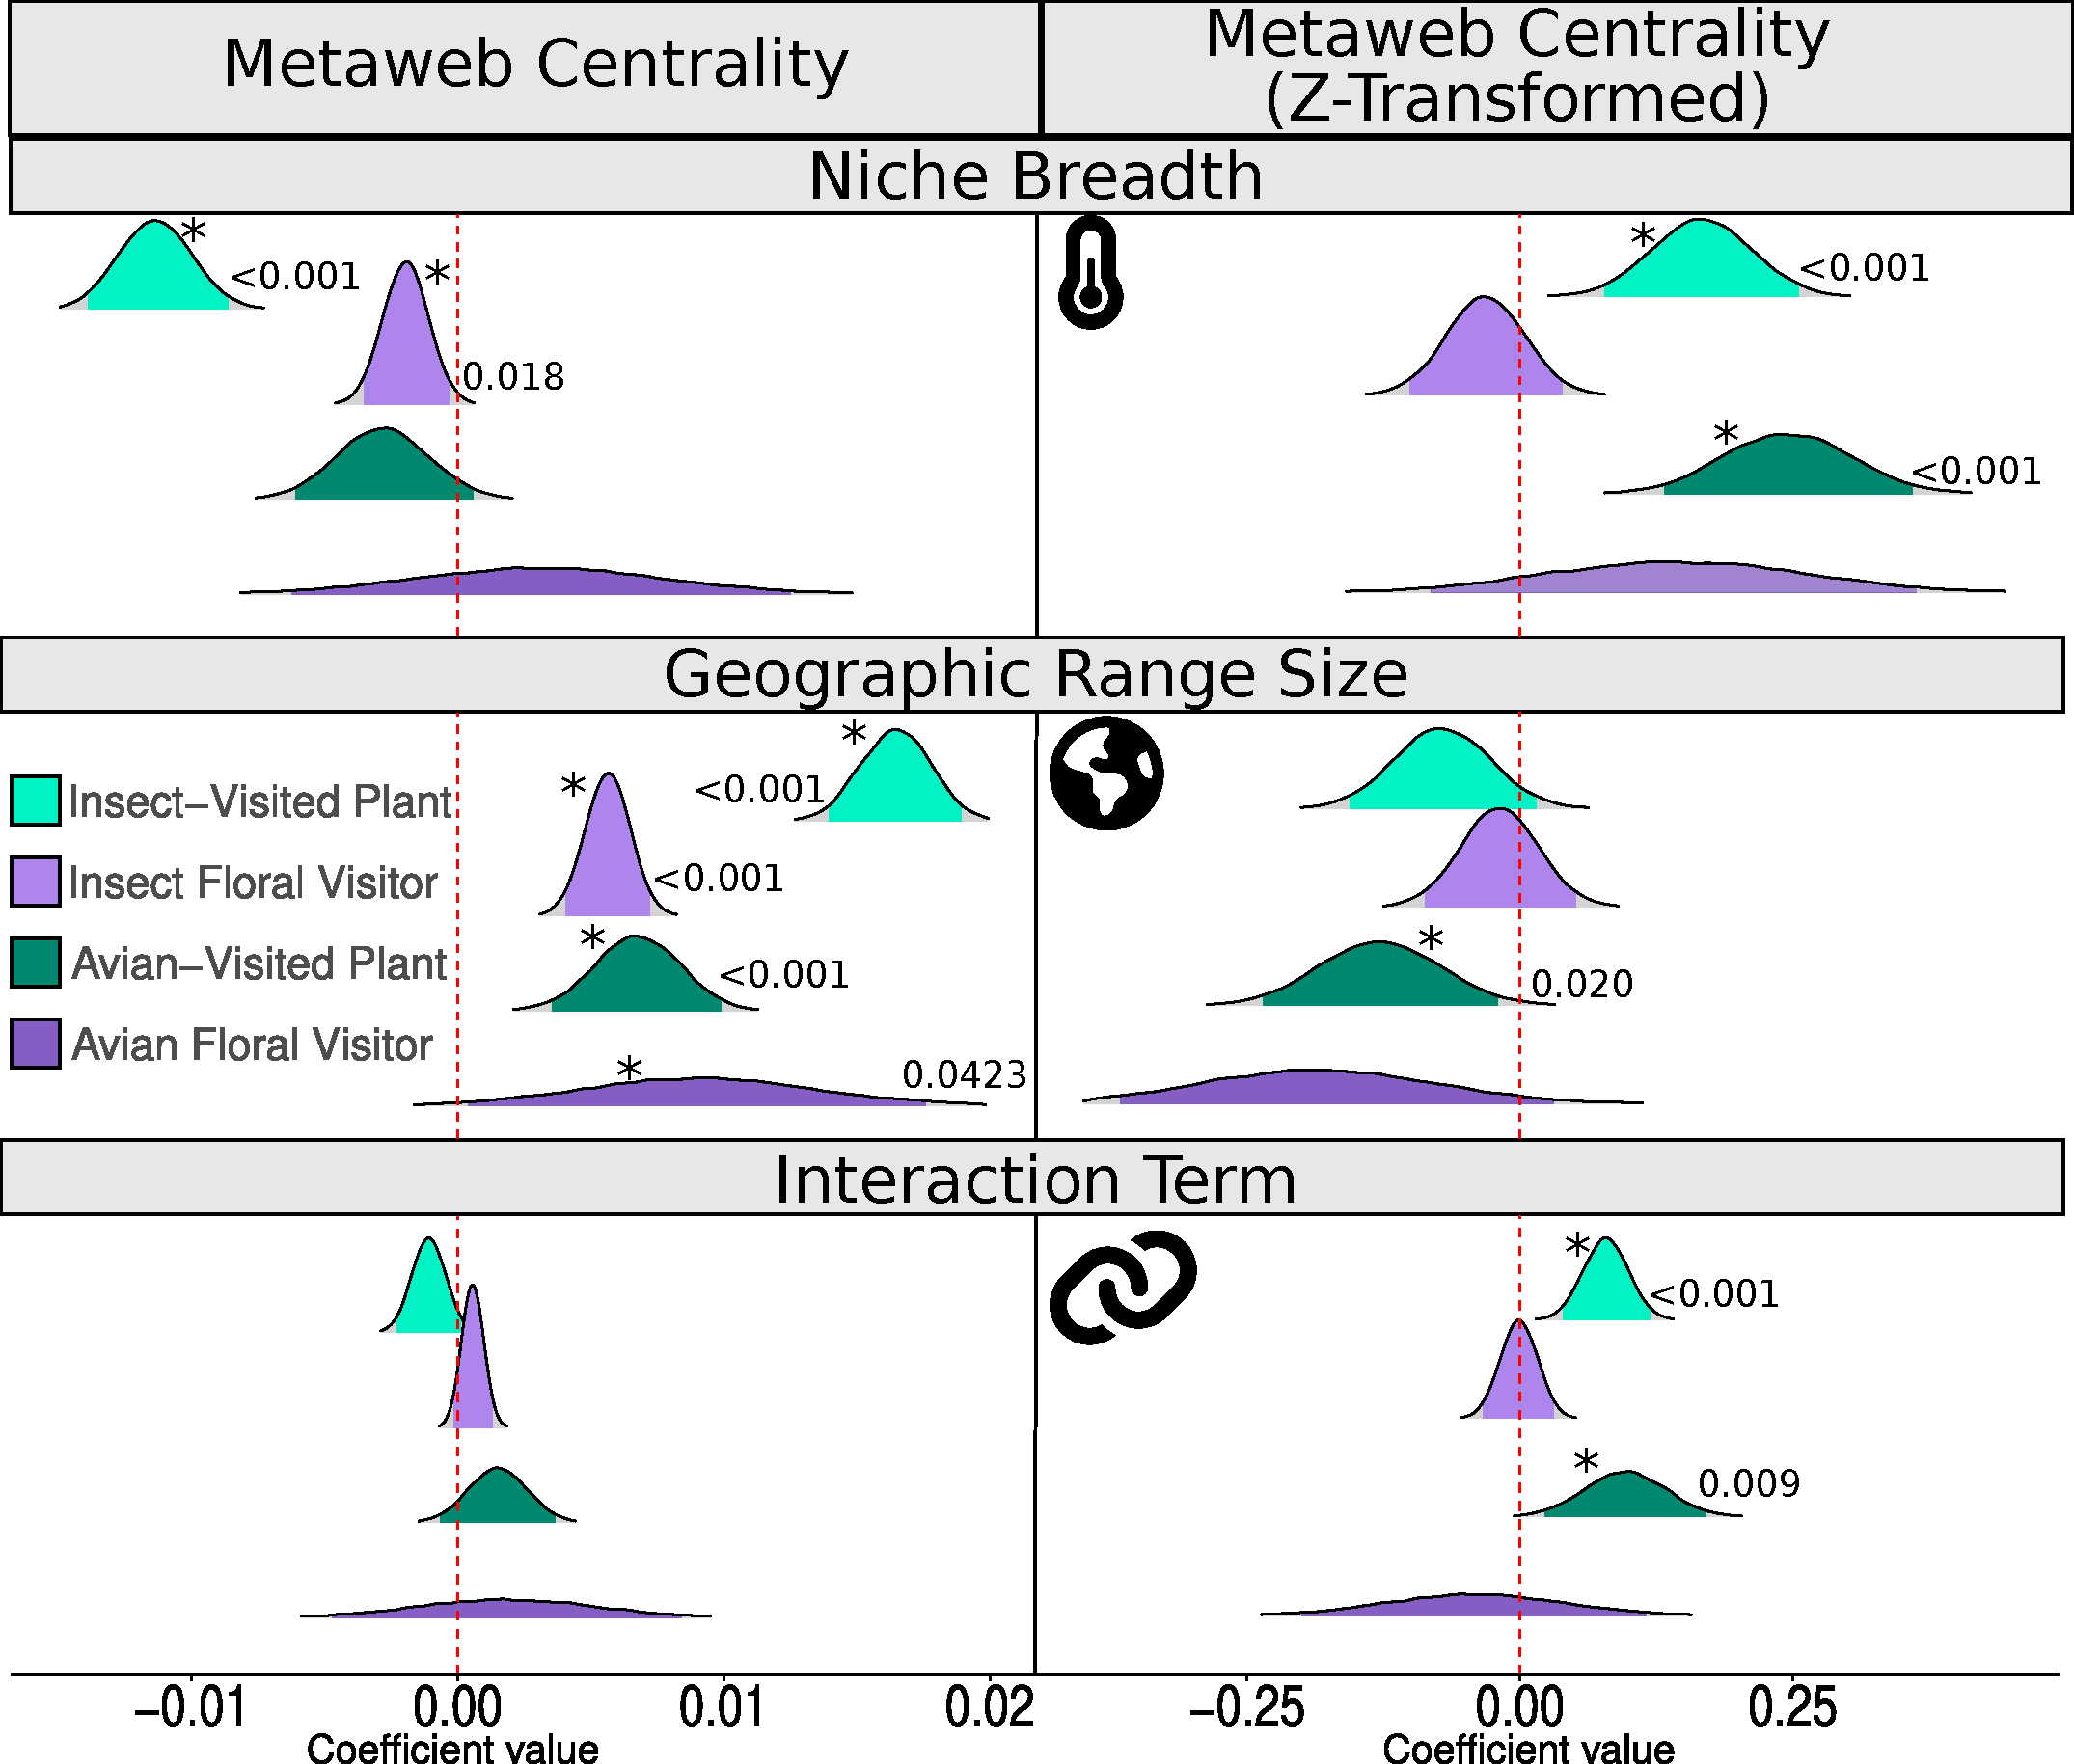
\includegraphics[width=\columnwidth, alt={Sampled posterior slope density curves for multivariate Bayesian generalized linear models of species centrality in the global metaweb}]{centralRange/figs/pdf/Effectplot_Metaweb_Updates.pdf}
    \caption[Sampled posterior slope densities for multivariate Bayesian generalized linear models of species centrality in the global metaweb]{Sampled posterior slope densities for multivariate Bayesian generalized linear models of species centrality in the global metaweb. Colored areas represent 95\% credible intervals of slope terms of the effect of niche breadth (top row, thermometer icon), geographic range size (center row, globe icon), and their interaction term (bottom row, chain icon).  Numbers and asterisks indicate approximate two-sided posterior probability $<0.05.$ Left columns represent models of measured closeness centrality as the response variable; right column represents models predicting centrality values $z-$transformed based on null randomization. After accounting for niche breadth, geographic range size has a strong positive effect of species centrality, but this effect disappears when z-standardized. In plant species, both niche breadth and the interaction between niche breadth and geographic range size positively impact $z$-transformed metaweb centrality.
    }
    \label{fig:MetawebEffect}
\end{figure}

\clearpage 

\begin{figure}[H]
\centering
    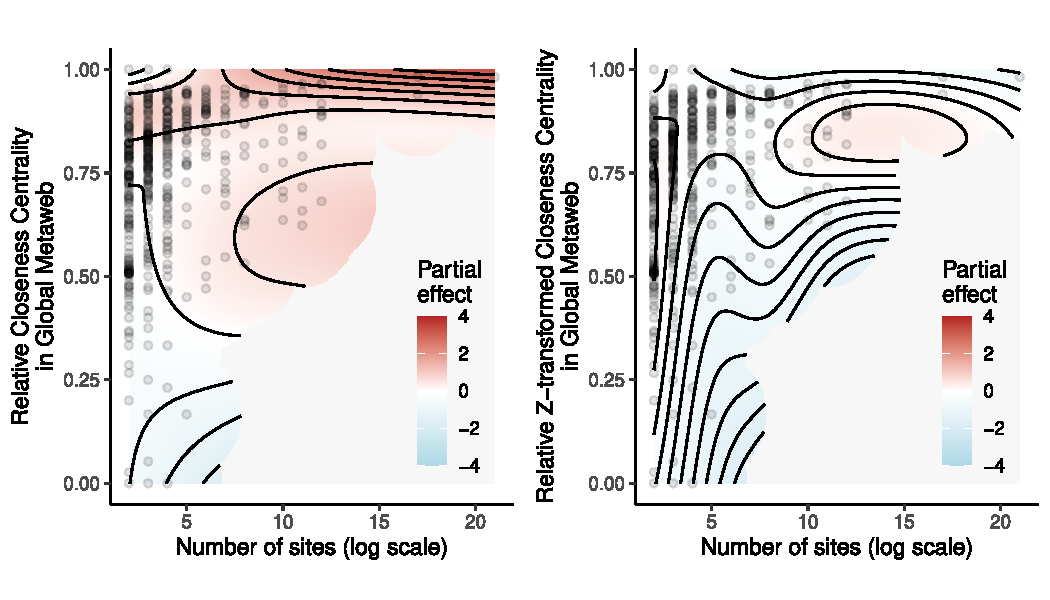
\includegraphics[width=\columnwidth, alt={Contour plot describing effects of interaction turnover on metaweb centrality}]{centralRange/figs/pdf/gamplot.pdf}%
    \caption[Partial effects of interaction turnover on metaweb centrality]{Partial effects of interaction turnover on measured metaweb centrality (left) or $z-$transformed metaweb centrality (right) response values and number of unique local sites, according to fit tensor product GAMs. For comparison, both responses are rescaled to mean of 0 and standard deviation of one. Across the observed range of centrality values, the tensor product of interaction turnover and number of local sites occupied by a species had a positive effect of global metaweb centrality ($p<0.001, R^2=0.231$), especially for the most highly central species. In contrast, after $z-$transformation while the tensor product of turnover and number of local sites a statistically significant negative effect, this relationship explained less than 6\% of variation in metaweb centrality ($p<0.001, R^2=0.054$).}
    \label{fig:gam}
\end{figure}
\clearpage 

\begin{figure}[H]
\centering
    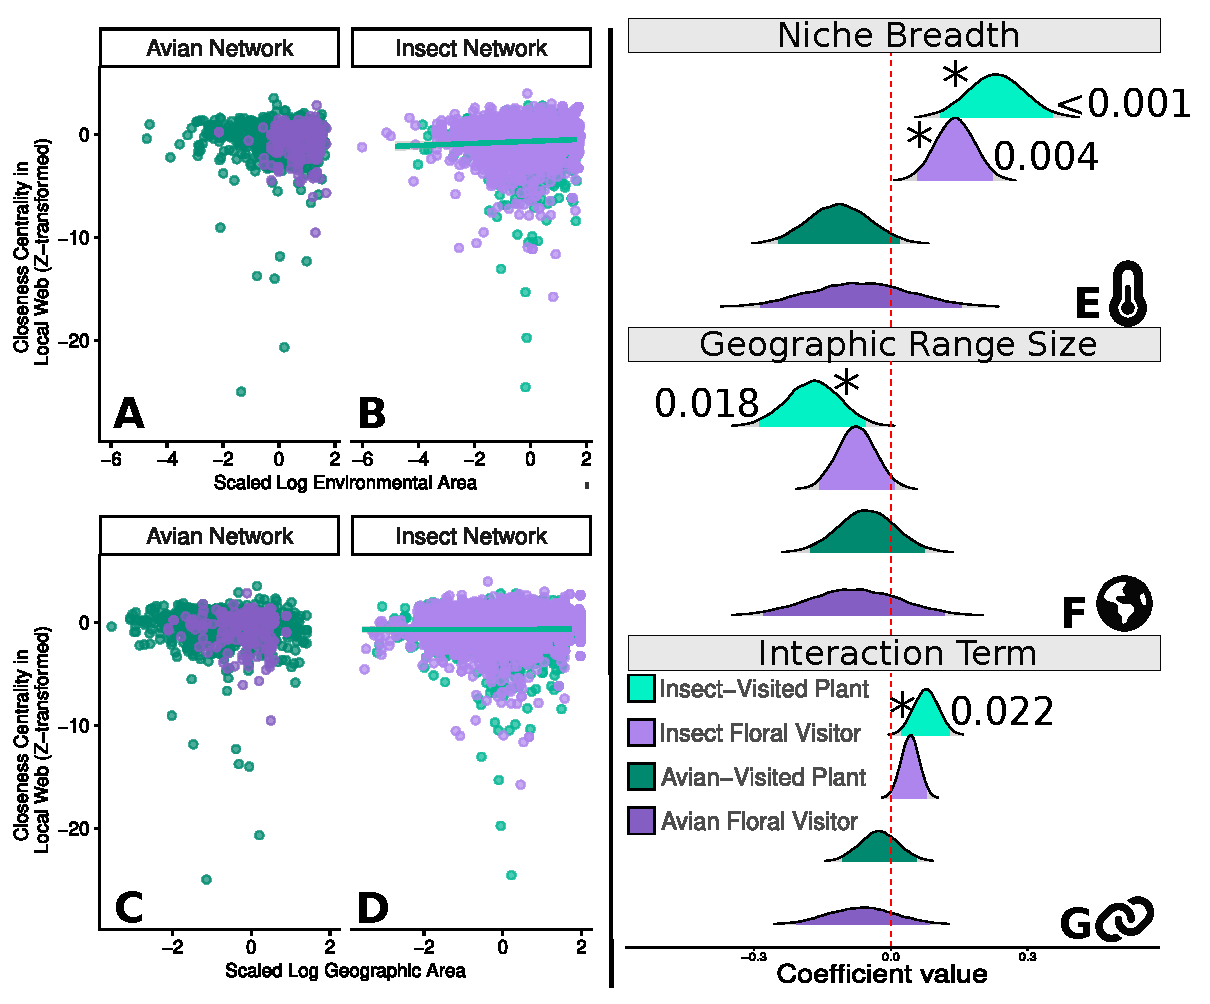
\includegraphics[width=6in, alt={Split figure, where the lefthand side is comprised of scatterplots describing the relationship between centrality in local networks and environmental or geographic range size. The righthand side gives posterior density curves of bayesian generalized linear models of these effects}]{centralRange/figs/pdf/LocalPlot_Composite_v2.pdf}%
    \caption[Relationships between average z-standardized centrality in local networks, geographic range size, and niche breadth]{Relationships between average z-standardized centrality in local networks, geographic range size, and niche breadth. Species-level closeness centrality ($z-$transformed) in local interactions networks as a function of geographic range size (A,B) or environmental niche breadth (C,D). Panels (E-F) show sampled posterior slope densities for multivariate Bayesian generalized linear models of average species $z-$transformed closeness centrality in local metawebs. Colored areas represent 95\% credible intervals; numbers and asterisks indicate approximate two-sided posterior probability $<0.05.$ Niche breadth had a positive effect on the local centrality only of both node types within insect networks (E). Additionally, we also observe a positive interaction between niche breadth and geographic range size on standardized centrality for these node types as well(G).}
        \label{fig:LocalPlot}
\end{figure}                                                                  

\addtocontents{toc}{\protect\vskip-20pt}
\chapter[Island biogeography of host-helminth interaction networks]{The impacts of geographic range size and niche breadth on species centrality in floral visitation networks\footnote{In revision at \textit{A GOOD JOURNAL, I PROMISE}. Reproduced here under the CC BY 4.0 license terms. See Appendix D.}}   



Island biogeography theory has been widely applied to predict properties of species assemblages across islands, but its relevance for species interaction networks remains less clear. Here, we take a macroecological approach to investigate how bipartite interaction networks between free-living hosts and helminth parasites vary across gradients of island area and isolation. Using the current largest published global collection of host-helminth interaction records, we tested the relationship between island characteristics and host richness, helminth richness, and interaction nestedness. We found that host and helminth richness were positively associated with island area and mainland connectivity as measured by surrounding landmass proportion, though unrelated to distance to the nearest mainland. In contrast, nestedness showed only a weak positive relationship with island area and was unrelated to mainland connectivity. These results suggest that island characteristics shape the size of host-parasite assemblages more predictably than the organization of interactions within them. Our findings extend island biogeographic perspectives to antagonistic interaction networks and motivate future work examining how host-mediated colonization and parasite specialization contribute to the assembly of antagonistic network structure across space.



\clearpage
%-----------------------------

%\subsubsection*{Island biogeography and how it blends well with current macroecological ideas}
\section*{\textbf{\underline{Abstract}}}
Island biogeography theory posits that island area and distance to the mainland combine to constrain species richness on islands through effects on extinction and colonization, respectively \citep{macarthur2001}. Despite being developed well over fifty years ago, it maintains an active research area, with numerous open questions \citep{patino2017}. This is perhaps a result of the ways that island biogeography theory can be used to inform other ecological relationships. For instance, island biogeography theory is quite closely linked to the examination of species-area relationships \citep{losos2000, peay2007}. Further, island biogeography theory is a simple base on which to build, as seen by extensions to species functional trait variation \citep{jacquet2017}, predator-prey interactions \citep{gravel2011}, and compositional differences between communities \citep{lu2018}. It is clear that island biogeography theory has the potential to inform trophic and community scale phenomena. 
\end{Abstract}


\subsection*{Introduction}
%\subsubsection*{Island biogeog and species interaction networks}
\paragraph*{}
The increasing availability of ecological data has encouraged the study of large-scale processes such as island biogeography theory. This data availability has also promoted the study of species interaction networks \citep{delmas2019, dormann2017}, which characterize the interactions between two (or more) trophic groups (e.g., plant species and their pollinators). This has permitted examinations into how spatial and environmental gradients influence the structure of these species interaction networks \citep{tylianakis2017}, with structure defined using measures such as nestedness and modularity \citep{dalsgaard2013, dormann2017}, which capture the tendency of species interactions to form proper subsets of species with more interactions (nestedness) or cliques of interacting species (modularity). Regardless of the measure used to capture aspects of species interactions, there is mounting evidence that species interactions follow the same patterns as species richness with regards to island area and isolation \citep{sugiura2010, dormann2017, tylianakis2017}. For instance, \citet{traveset2016} compared mainland and island plant-pollinator networks, finding that isolated oceanic islands had the lowest species richness -- in agreement with predictions from classic island biogeography theory -- and the lowest interaction diversity and highest plant niche overlap. That is, as the richness of plants and pollinators decreased with isolation, so did the structure of the interactions between plant and pollinator species. Relatedly, \citet{dalsgaard2013} found that species interaction networks tended to be modular on islands, further linking island biogeography with the study of species interaction networks. But how do we interpret the effects of island isolation and area on species interactions?




%\subsubsection*{How is the original theory related to network structure?}
\paragraph*{}
Classical biogeography studies posit that the species richness of oceanic islands is largely determined by the equilibrium between species colonization and extinction rates. Islands closer to mainland sources are colonized by new species at a higher rate, while islands with larger areas exhibit lower extinction rates. However, the interpretation of the influence of island isolation and area on the structure of species interaction networks must be different. That is, the richness of interacting species, even if driven by a balance between colonization and extinction rates, should not necessarily influence the overall structure of species interactions. For instance, if species interactions are conserved between mainland and island populations -- as evidenced by \citet{carstensen2018} -- then differences between mainland and island species interaction networks should be minimal. However, there are other reasons why island area could influence network structure. Larger islands tend to have more diverse habitat types than smaller islands, and species habitat preferences can contribute to modularity of interaction networks by reducing niche overlap between groups of habitat specialists \citep{santos2016}. Meanwhile, island isolation, as noted above, is likely unrelated to network structure, provided that species interactions are not overly plastic (i.e., species cannot readily change the set of species they interact with), or that species dispersal ability is directly related to specialization (i.e., good dispersers interact with many species).






%\subsubsection*{Thesis}
\paragraph*{}
It may be infeasible to provide tests of the underlying mechanisms which drive relationships between island isolation or area and properties of species interaction networks. However, demonstrations of the existence of the scaling relationships themselves are useful in identifying groups of species or types of interactions which modify the strength or directionality of effect of island characteristics on species interactions. For instance, while studies examining mutualistic network structure across islands are becoming increasingly common \citep{traveset2016, dalsgaard2013, sugiura2010, trojelsgaard2013}, comparable studies of antagonistic networks have lagged behind (but see \citep{gravel2011}). However, antagonistic and mutualistic networks often have quite different structural properties, potentially owing to the intrinsic difference in the effect of the species interaction (i.e., the cost of parasitism and the benefits of mutualism). Here, we examine the relationship between host-parasite network structure and island isolation and size, using host-helminth interaction data from 61 islands. First, we examined the relationship between species richness and island isolation and size, in accordance with traditional island biogeography theory. Second, we examined how a key measure of ecological network structure, interaction nestedness, scales with island characteristics. Overall, our findings suggest that while the diversity of host-parasite assemblages varies predictably with island characteristics, the structure of their interaction networks shows a more limited association. Reconciling the differences between mutualistic and antagonistic network structures among islands may provide insight into how island isolation and area are mechanistically related to species interactions and network structure.














%----------
\section*{Methods}

\subsubsection*{Host - helminth interaction data}
Records of helminth parasite occurrence on host species were obtained from the parasite database of the London Natural History Museum (LNHM) \citep{gibson2005}, and accessed programmatically using the \texttt{helminthR} package \citep{helminthr}. These data currently represent one of the largest sources of host-parasite interaction data \citep{dallas2018}, despite being restricted to helminth parasites, including Platyhelminthes (trematodes and cestodes), Acanthocephalans, and Nematodes \citep{gibson2005}. We started by identifying a total of 62 islands for which host-helminth interaction data were recorded (Figure \ref{fig:concept}). After filtering out host and helminth species not identified to the species level, this comprised a total of 7294 host-helminth species pairs across 2651 helminth species and 1980 host species.


\subsubsection*{Island isolation and size measurement}
Data characterizing the geography of islands were retrieved from \citep{Weigelt2013}, including island area (km$^2$). We measure island isolation through distance to the nearest mainland (km), and surrounding landmass proportion (SLMP), calculated as the proportion of land area within 100, 1000, and 10,000 km buffers. This metric accounts for both spatial variation in mainland connection as well as nearby island connections, and has been shown to be more robust than distance per se in explaining insular plant diversity \citep{weigelt2013quantifying}. To roughly account for historical connectivity, we also extract whether or not an island had terrestrial connections to the mainland during the last glacial maximum (GMMC). Records within the LNHM dataset were georeferenced to an island chain or series (e.g. Trinidad \& Tobago) were assigned to the largest island within the group (e.g. Trinidad). Data from \citep{Weigelt2013} were available for all but one island in our data (South Shetlands), an Antarctic island with only seabird and pinniped infection records, which we excluded from our analysis. 


\subsubsection*{Quantifying host-helminth network structure}

We related island characteristics to both species richness estimates and to measures of interaction network structure. Measures of species richness for both hosts and helminths were obtained from the London Natural History Museum data, as described above. To quantify network structure, we estimated interaction nestedness, a commonly measured aspect of network structure found to be related to network structural stability \citep{thebault2010stability, dallas2015co, valdovinos2019mutualistic} and resilience \citep{thebault2010stability, suweis2013emergence}. However, some measures of nestedness may be related to network size (number of interacting species)\citep{bascompte2003nested, nielsen2007ecological}, which creates an odd circularity where a significant effect of island area or isolation on species richness would automatically manifest in an effect on network structure. 


One method for addressing the difficulty in comparing network structure measures between networks is to measure the difference between the empirical statistic and a distribution of the statistic obtained from null model randomization. This procedure has recently been criticized as not removing the effects of network size \citep{chagnon2015}, specifically for nestedness \citep{strona2014, song2017some}. Instead, we opted to use $NODF_c$, a normalized version of the classic nestedness metric based on overlap and decreasing fill proposed by \citet{song2017some}. Calculated as $NODF_c = NODF_n/(C\cdot \log(S))$, where $NODF_n$ represents the relative observed connectance of a given graph given its maximum possible value ($NODF/max(NODF)$), and $C$ and $S$ represent the connectance and the geometric mean of the number of nodes of each class, respectively. \citet{song2017some} show that this normalized metric is insensitive to network size, and thus appropriate for comparing network structure across biogeographic scales. Computation of the $NODF_c$ was performed using a hill-climbing algorithm as implemented in the $maxNODF$ package \citep{hoeppke2021maxnodf}. For some networks with a small number of interacting species, the set of possible network configurations is too small to make meaningful inference; as such we excluded islands with five or less species within their networks ($n$ = 12). Across the remaining 47 islands, most contained networks with multiple disconnected components (modules of species with no direct linkages that connected them, $n$ = 35). As NODF is not directly measurable in disconnected networks, for networks containing multiple connected components we added the minimum number of links necessary to create a single component when calculating the maximum potential NODF value \citep{hoeppke2021maxnodf}. We demonstrate in the Supplemental Materials how the use of network structure measures that contain the influence of network size would lead to incorrect conclusions regarding the influence of island area and isolation on network structure. 

\paragraph*{Statistical Analysis}
Relationships between species richness and island characteristics were modeled as multivariate negative binomial regressions as implemented in the MASS package \citep{MASS2002}. We utilized negative binomial regressions as both Poisson and Quasi-poisson regression models exhibited significant overdispersion (see Supplemental Materials). As our alternative metrics of isolation (log distance to mainland and SLMP) were significantly negatively correlated ($\rho$ = -0.768, $p$ = 1.94e-12), we did not include both in the same model and instead used AIC to compare across metrics. The impact of island characteristics on the $NODF_c$ was modeled as a multivariate linear model using a Gaussian error distribution and logit link. Model fits were inspected through analysis of deviance and visual inspection of standard model diagnostic visualizations. Models of the effect on historical mainland connectivity (GMCC) on diversity and network characteristics were fit separately under the same framework as described above, as well as through a Wilcoxon signed-rank test. 


%-----------------------------
\section*{Results}

\subsubsection*{Species richness and island characteristics}
Island biogeography theory predicts that species richness will be negatively related to distance from a mainland (as a result of low dispersal success to distant islands), and positively related to island area (larger islands support more "stable" populations). We find evidence for an influence of area on species richness of both hosts ($\beta = $ 0.419, $p =$ 2.43e-12) and helminths ($\beta =$ 0.391, $p <$ 1.42e-10). Interestingly, host and helminth richness increased at nearly the same rate with island area. In contrast to the influence of island area, we failed to detect any influence of distance to the mainland on host ($\rho = $ -0.189, $p =$ 0.182) or helminth ($\beta = $  -0.221, $p =$ 0.116) species richness (Figure \ref{fig:islandBG}). However, when accounting for island connectivity through SLMP, we detected a positive relationship between surrounding land area and richness of both hosts ($\beta=$1.54, $p=$0.00161) and helminths ($\beta=$1.74, $p=$0.000262). 


\subsubsection*{Network structure and island characteristics}

Many measures of nestedness are sensitive to the effects of network size. In this case, network size is the species richness of host and parasite species in the network, which we found to be related to island area and SLMP (but not distance to the mainland; Figure \ref{fig:islandBG}). Using a nestedness measure that is related to network size would therefore lead to the conclusion that network structure follows a similar gradient as species richness (see Supplemental Material). Here, we use a measure of nestedness that is insensitive to network size, $NODF_c$. Using this measure, we detect a positive relationship between island area and interaction nestedness; larger islands have more nested host-helminth networks ($\beta$=0.325, $p=$0.0473, Figure \ref{fig:networkBG}). We failed to detect any relationship between network nestedness and maximum elevation, distance to mainland, or SLMP. 


% TAD: check results for tense issues. I've fixed a bunch of switches from past to present tense above, but I might have missed one or two. 




%Lastly, there was no clear spatial gradient in nestedness, suggesting that latitude or spatially-autocorrelated environmental variation are unlikely to drive network structure (Figure \ref{fig:nestMap}). This supports previous findings that antagonistic networks tend to be structured independently of latitude \citep{morris2014}.

%Grant Q: Do we still want to include this? I like it, but I don't know if that + the GMMC stuff is too many figures. 

\subsection*{Prehistoric Connectivity}

Independent of contemporary island area or distance to mainland, historical landbridge connections may alter species assemblages or network characteristics by influencing dispersal processes. We found that islands that had terrestrial mainland connections during the last glacial maximum tended to have higher host ($\beta=$1.61, $p=$9.58e-05) and helminth diversity ($\beta=$1.59, $p=8.11e-05$, Figure \ref{fig:GMMC}). Despite differences in richness, interaction networks did not differ in nestedness across GMMC status ($p=$0.71).  




%-----------------------------
\section*{Discussion}

\paragraph*{} Overall, the relationships we observed between island characteristics and the species richness of both hosts and helminth parasites are broadly consistent with predictions from classical island biogeography theory for free-living species, but nestedness showed a more limited pattern, responding weakly to island area and not to either measure of island connectivity. This suggests that island characteristics shape the size of host-parasite assemblages more predictably than they shape the organization of interactions within those assemblages. The framework of island biogeography predicts higher species richness on larger islands, in part because larger areas can support larger populations and thus lower extinction rates \citep{macarthur2001}, as well as greater habitat heterogeneity that accommodates a wider diversity of species \citep{triantis2008measurements, hortal2009island, macdonald2018theory}. Consistent with these expectations, we find a significant positive correlation between island area and the species richness of both hosts and helminths \ref{fig:islandBG}. 

\paragraph*{} Classical theory also predicts reduced diversity on islands that are more isolated from mainland source pools due to lower colonization rates \citep{macarthur2001}. While we do not detect a direct effect of distance to the mainland on species richness, we do observe a significant positive relationship between species richness and island connectivity, as measured by surrounding landmass proportion (SLMP), for both hosts and helminth parasites. Although distance and connectivity are related metrics, SLMP incorporates both proximity and the size and configuration of surrounding landmasses (including large neighboring islands), and may therefore provide a more accurate proxy for colonization potential \citep{Weigelt2013, weigelt2013quantifying, barreto2021area}. 

\paragraph*{} Species interaction networks on larger islands tend to be more nested than those on smaller islands \ref{fig:networkBG}, but this effect was generally weak ($R^2 = $0.086). In diverse communities, patterns of asymmetric specialization (i.e., specialist parasites tend to interact with hosts with high parasite richness, while the parasite communities of hosts with few associated parasites are dominated by generalist species) results in interaction nestedness \citep{vazquez2005species, lima2012patterns}. Significant interaction nestedness has been observed in a number of parasitic systems \citep{krasnov2011nestedness, lima2012patterns, guerra2016host}, and island host-helminth networks may be smaller subsets of more regionally nested source networks. If so, larger islands may more closely reflect the structural properties of these regional pools, while the comparatively depauperate networks of smaller islands may not fully preserve this nested architecture. Alternatively, the relationship between island area and nestedness may reflect non-random assembly if colonization or extinction probabilities are associated with host or parasite specialization. For example, parasites with broad host ranges, high prevalence, or those associated with abundant or highly mobile hosts may be more likely to colonize and persist on islands, while specialist parasites may be disproportionately absent from smaller islands.  

\paragraph*{} While some attention has been paid to the island biogeography of mutualistic networks \citep{sugiura2010, dalsgaard2013, traveset2016, nogales2024review}, the processes underpinning them are fundamentally different. Among these is the role of co-colonization. In many mutualistic networks, potential interaction partners may disperse and establish on islands relatively independently. In contrast, helminths generally have much lower dispersal capacity than their free-living hosts \citep{poulin2004macroecological}. As such, the dispersal of parasites to new islands is largely dependent on patterns of host dispersal \citep{font2003global, bataille2017colonization}. Parasites that have high prevalence of infection or broad host ranges may be more likely to colonize new islands. For example, parasites with sufficiently broad ranges may be able to disperse to new areas via transient hosts, even if those species do not establish persistent populations on a given island (\citet{ellis2023host} give an example with avian malaria). Alternatively, specialist species with close host associations may be more likely to be retained during colonizations \citep{schatz2023patterns}. Thus, generalist parasites may have more opportunities to colonize new islands, while some specialists may be more likely to persist when their hosts successfully establish, making the relationship between specialization and colonization potential non-linear. These linkages between host range and colonization potential may induce a biotic filter that ultimately affects network structural properties. Understanding how parasite colonization dynamics scale up to affect resulting species interaction networks across gradients is an outstanding question. 

\paragraph*{} The mechanisms underlying island-area effects on host-helminth network structure remain difficult to resolve in part because parasite occurrence and interaction data may be shaped by both biological features and sampling limitations \citep{nielsen2007ecological, llopis2023sensitivity}. The sampling of parasite communities is inherently difficult, and is limited by the availability of survey effort and taxonomic expertise. Additionally, for many helminth taxa, we have incomplete information about which hosts they are capable of infecting in nature, making it difficult to determine whether unobserved interactions represent true absences or merely incomplete sampling \citep{poulin2016missing, walker2017uncertain, farrell2022predicting}. As a result, the networks analyzed here are unlikely to represent complete characterizations of island host-helminth communities, especially on very small islands with limited sampling effort or very large islands with highly diverse host and parasite faunas. More complete and effort-standardized surveys of host and parasite communities, paired with better characterization of helminth host ranges through surveillance and experimental infection studies, may help clarify the mechanisms determining parasite colonization, persistence, and network structure across biogeographical gradients.

\paragraph*{} However, in their current form, large-data repositories like the London Natural History Museum \citet{gibson2005} still provide the opportunity to investigate the structure of parasitic communities at macroecological scales, and can motivate these further data collection efforts. To our knowledge, ours is the first study to examine the structural properties of host-parasite networks in an island biogeography context. The increasing availability of open species interaction data spanning wide geographic, taxonomic, and temporal scales provides new opportunities to better understand large-scale determinants of network structural properties and their consequences for community assembly. By looking across geographic and environmental gradients, we show that island characteristics may shape the size of host-parasite assemblages more predictably than the organization of interactions within them, while also highlighting the need to understand how host-mediated colonization shapes antagonistic network structure across environments.

\clearpage 
\bibliographystyle{plainnat} 
\bibliography{var} 
\clearpage


\section*{Figures}


\begin{figure}[h!]
  \begin{center}
    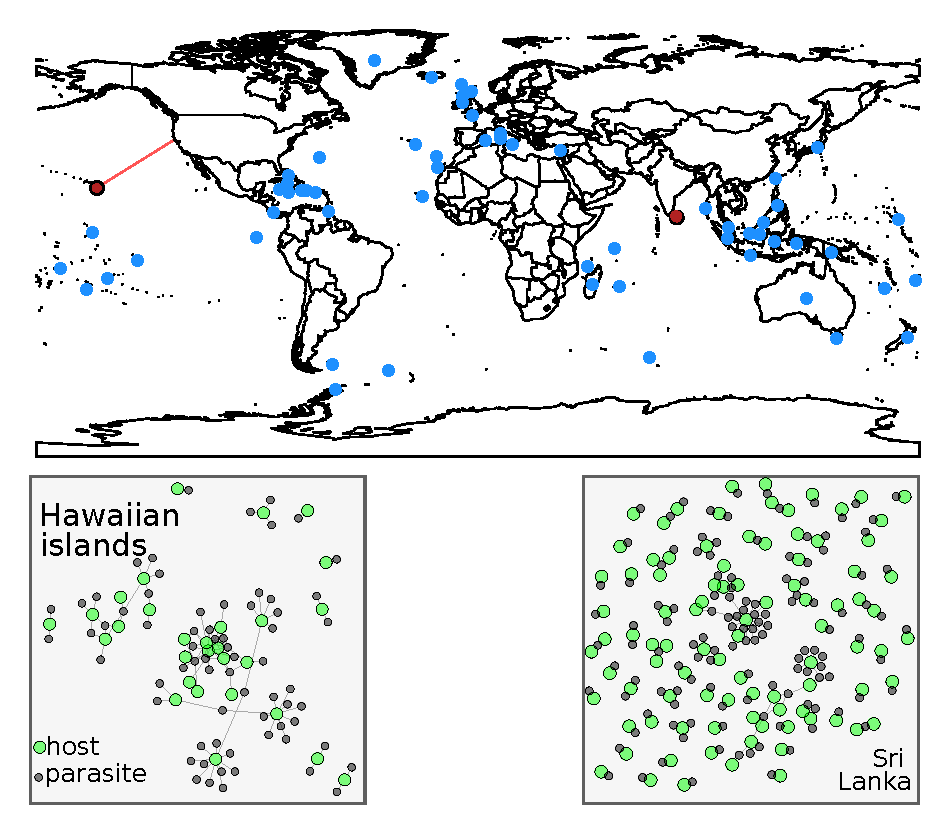
\includegraphics[width=\textwidth]{HelmBiogeog/Figures/conceptual/concept.pdf}
    \caption{Both distance to mainland and island area may influence species richness and host-helminth network structure. Islands considered in the analysis are in blue, with two example networks from the Hawaiian islands and Sri Lanka highlighted in red. Hawaii is much smaller and more distant to the mainland, and also has lower species richness relative to Sri Lanka. }
    \label{fig:concept}
  \end{center}
\end{figure}

\clearpage


\begin{figure}[h!]
  \centering
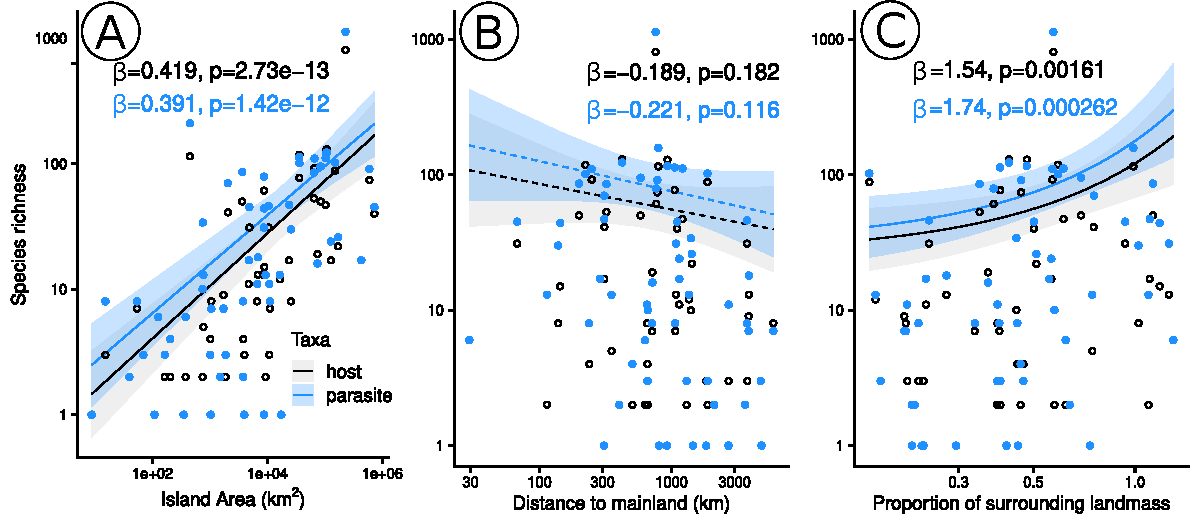
\includegraphics[width=\linewidth]{HelmBiogeog/Figures/NB_MarginalPlots_Wide.pdf}
  \caption{Traditional island biogeography theory relates species richness to the distance to the mainland (i.e., isolation) and island area. We detect a significant positive effect of island area on both helminth parasite and host richness (A), but found no significant effect of isolation as measured by distance to mainland (B). When measuring island isolation through surrounding landmass proportion, we did detect a weak but significant positive effect of island connectivity on both helminth and host richness (C). Plotted lines represent fitted relationships from a negative binomial multivariate regression model, assuming mean values of non-focal predictor variables. Significant relationships represented as solid lines; shaded regions represent 95\% confidence intervals.}
  \label{fig:islandBG}
\end{figure}

\clearpage

\begin{figure}[h!]
  \begin{center}
    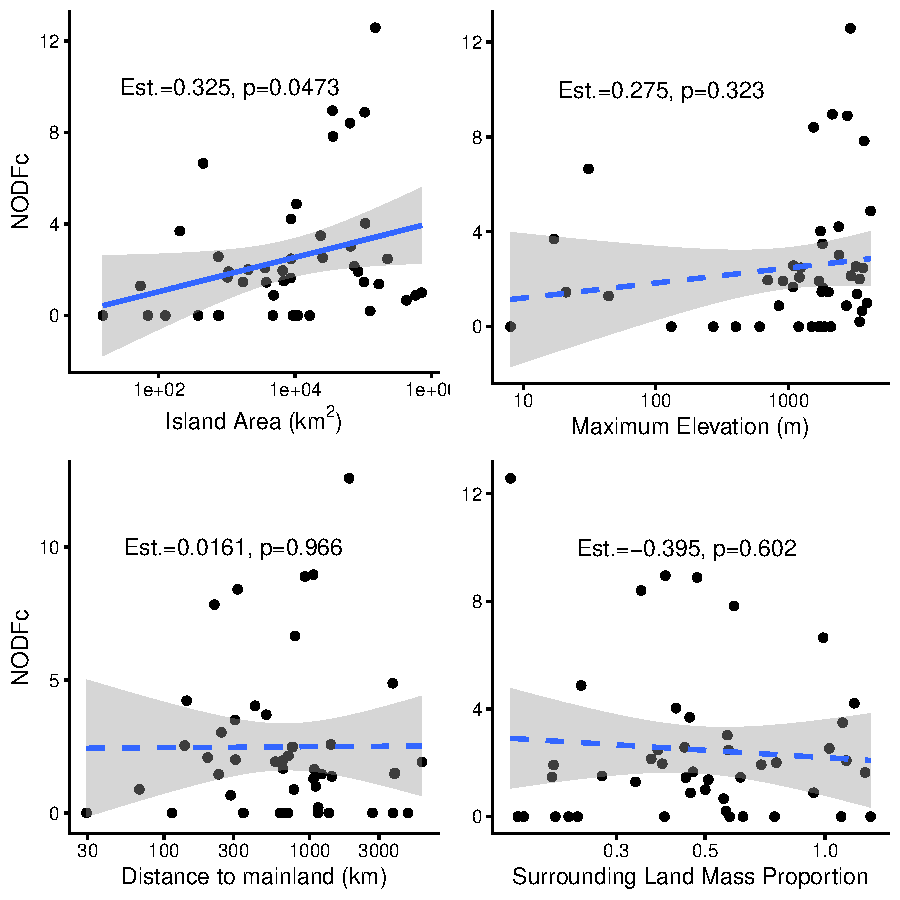
\includegraphics{HelmBiogeog/Figures/NODFc_plots.pdf}
    \caption{In addition to impacting network size, island area was positively related to $NODF_c$ such that larger islands were tended to be more nested on average (top left). In contrast, neither island elevation (top right) nor measures of island isolation including distance from the mainland (bottom left) or SLMP (bottom right) were significantly related to interaction nestedness within island networks.} %GF: Still need to add labels as well as fix cut off island area x-axis
    \label{fig:networkBG}
  \end{center}
\end{figure}

\clearpage


\begin{figure}[h!]
  \begin{center}
    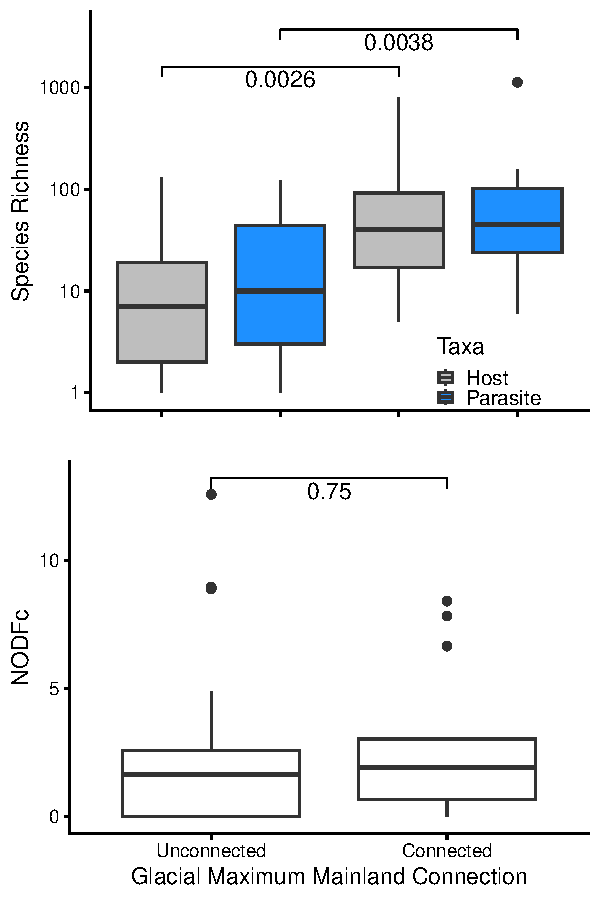
\includegraphics{HelmBiogeog/Figures/GMCC_NODFc_boxplots.pdf}
    \caption{Islands with a terrestrial connection to the mainland during the most recent glacial maximum have significantly higher host and helminth parasite diversity (top), but exhibit no significant differences in network nestedness. Comparison labels indicate p-values from a pairwise Wilcoxon test.}
    \label{fig:GMMC}
  \end{center}
\end{figure}













%--- Supplement ---

\clearpage

\section*{Supplemental Material}

\title{Island biogeography of host-helminth interaction networks}

\author[a,*]{Grant Foster}
\author[a,b]{Tad A Dallas}
% TAD: I don't think this will actually work, so maybe just write it out instead of trying to format it like main text. 

\affil[a]{Department of Biological Sciences, University of South Carolina, SC 29208, USA}
\affil[b]{Center for the Ecology of Infectious Diseases, University of Georgia, Athens, GA, 30602}


\renewcommand\Authands{ and }
\date{ \small *Corresponding author: grant.t.foster500@gmail.com}



\beginsupplement



\subsubsection*{The relationship between network size and nestedness}

Disentangling species richness (the sum of host and parasite richness) from nestedness is difficult, and many nestedness measures scale with species richness (Figure \ref{fig:richnessEffect}). Comparisons of properties across networks of different sizes is a non-trivial problem, and one potential solution is the implementation of a null modeling approach. In our case, we repeatedly shuffle links between hosts and helminths in each network, while maintaining both parasite host range (i.e., the number of host species a given parasite infects), and parasite species richness (i.e., the number of parasite species a host is infected by). For each network, we produced 1000 randomized networks, creating a distribution of spectral radii. Using these null distributions, we calculated $z$-scores, which measure the degree of divergence of the empirical network from the randomized null networks. Below, we present the correlations between alternative measures of network nestedness ($\eta$\citep{jonhson2013factors}, spectral radius, NODF, and $NODF_c$) as well as z-transformed versions of NODF and spectral radius. Nestedness as measured by $\eta$ was not standardized, as null model randomization for this measure is difficult, as randomized networks maintaining aspects of the degree distribution of host and parasite species will result in the same $\eta$ value as the empirical network. 

We find a significant correlation between the log-scale number of species within a network and all of the most common measures of network nestedness. However, as shown by \citet{song2017some}, $NODF_c$ is unrelated to network size or connectance across large sets of randomly generated networks. The relationship we observe across island networks may therefore reflect covariance with island area rather than a direct effect of network size on nestedness. Island area is positively associated with both network size \ref{fig:islandBG} and network nestedness \ref{fig:nestMod}, suggesting that area may act as a shared underlying driver that confounds the apparent association between network size and nestedness. As such, using metric sensitive to network size may give conflicting results. \ref{fig:Spectral.z_Results} illustrates that when using z-standardized NODF as our measure of interaction nestedness, we see the opposite relationship between island area and nestedness as with our $NODF_c$ metric, as well as relationships with elevational range and SLMP. In contrast, measuring interaction nestedness by the z-standardized spectral radius of a given graph yields qualitatively similar results to $NODF_c$ \ref{fig:Spectral.z_Results}.  

\begin{figure}[h!]
  \begin{center}
    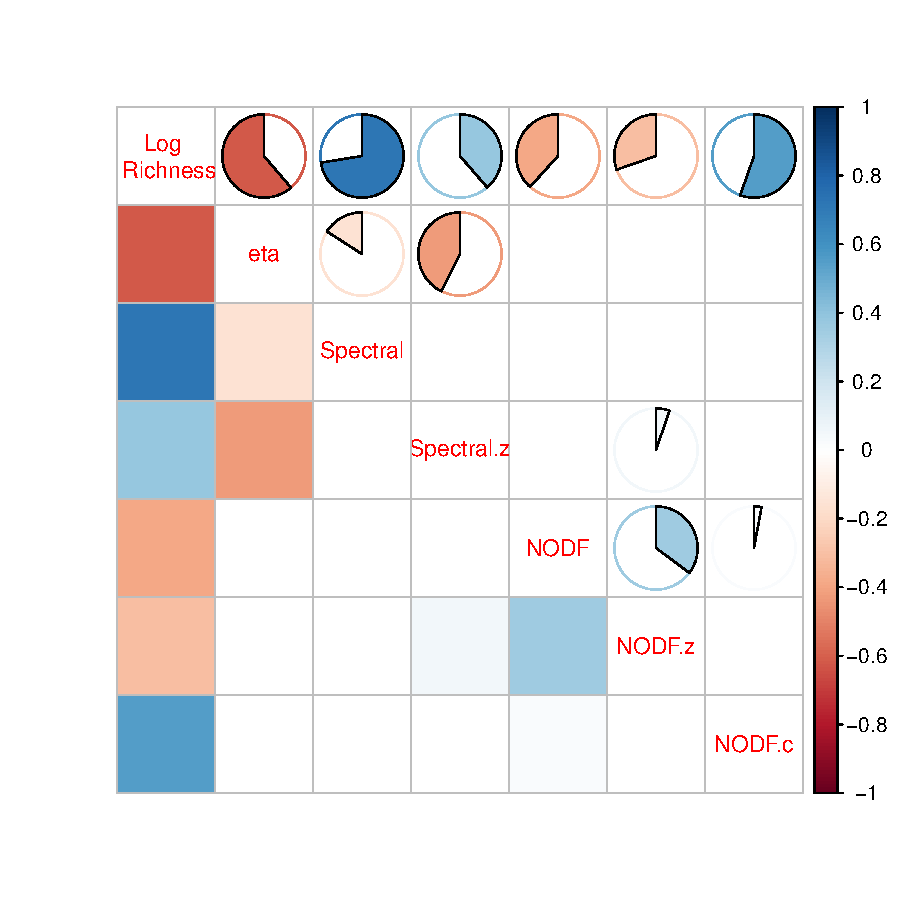
\includegraphics[width=\textwidth]{HelmBiogeog/Figures/Netsize_corplot.pdf}
    \caption{Correlogram visualizing Pearson's correlation coefficients between network size (log species richness) and alternative measures of network nestedness in our data. Shaded squares represent significant correlations (p-value $<0.05$). All measures of nestedness ($\eta$\citep{jonhson2013factors}, spectral radius, and NODF, as well as z-scores of the latter two based on null randomizations) are significantly correlated with network size in our dataset}
    \label{fig:richnessEffect}
  \end{center}
\end{figure}


\begin{figure}[h!]
  \begin{center}
    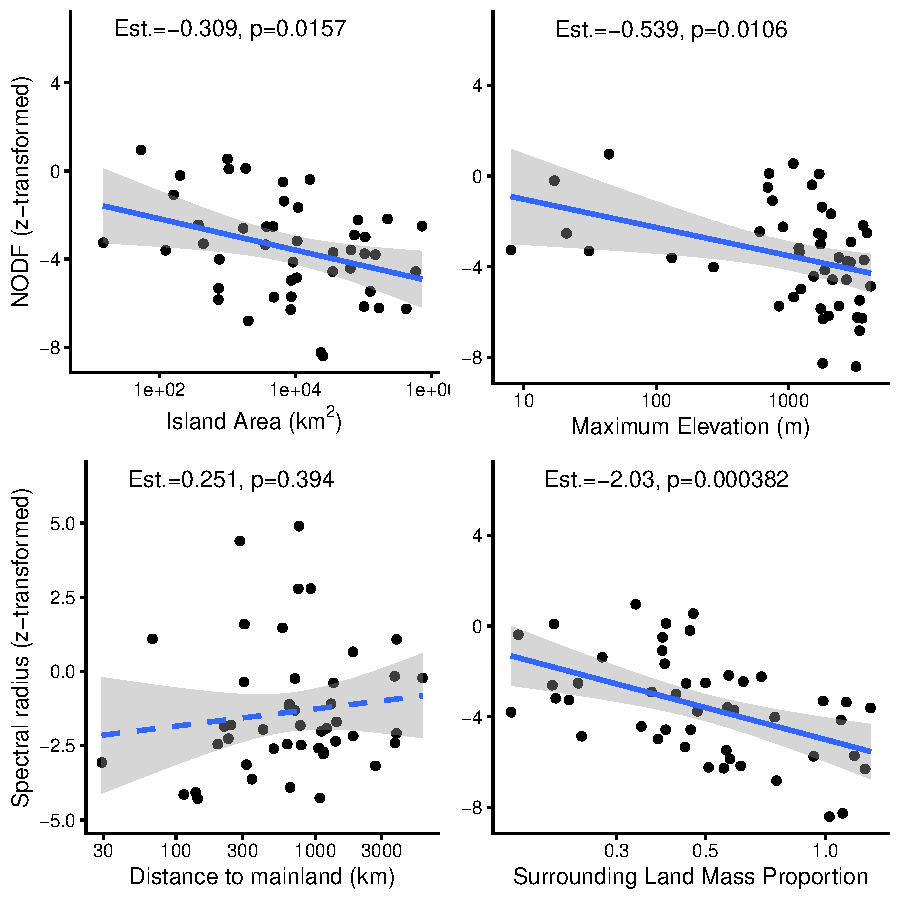
\includegraphics[width=\textwidth]{HelmBiogeog/Figures/NODF.z_Plots_Supplement.pdf}
    \caption{Recreation of Figure \ref{fig:networkBG} of the main text using z-transformed NODF as our nestedness metric of comparison. Despite null modeling approaches, this metric may still be sensitive to network size, and this gives conflicting results to those observed in $NODF_c$. }
    \label{fig:NODF.z_Results}
  \end{center}
\end{figure}

\clearpage

\begin{figure}[h!]
  \begin{center}
    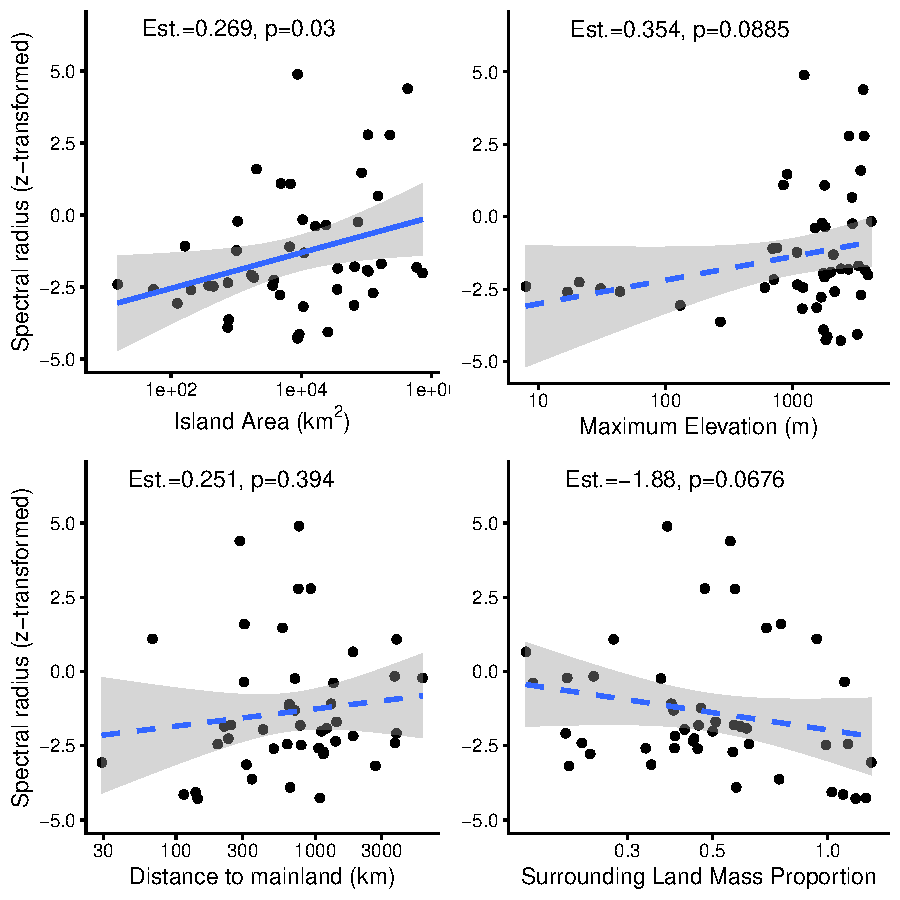
\includegraphics[width=\textwidth]{HelmBiogeog/Figures/Spectral.z_Plots_Supplement.pdf}
    \caption{Recreation of Figure \ref{fig:networkBG} of the main text using z-transformed spectral radius as our nestedness metric of comparison. In contrast to z-standardized NODF, spectral radius yields qualitatively similiar results to $NODF_c$ after z-transformation.}
    \label{fig:Spectral.z_Results}
  \end{center}
\end{figure}


\subsubsection*{Statistical Analysis}

In the main text, we use a negative binomial modeling multivariate regression approach to model the effects of island characteristics on species diversity. This approach greatly minimizes residual deviance compared to both Poisson and Quasi-Poisson GLMs \ref{tab:host_div_deviance}. Models incorporating island area and isolation as measured by SLMP yielded lowest AIC values, and as such are presented in the main text. 

\begin{table}[ht]
\centering
\caption{Model deviance diagnostics for host diversity models.}
\label{tab:host_div_deviance}
\begin{tabular}{lrrrr}
\hline
Model & Residual deviance & Residual df & AIC & Deviance/df \\
\hline
Poisson: Area + SLMP & 5621.91 & 55 & 5873.20 & 102.22 \\
Quasi-Poisson: Area + SLMP & 3497.06 & 55 & -- & 63.58 \\
Negative binomial: Area + Distance & 65.10 & 55 & 488.86 & 1.18 \\
Negative binomial: Area + SLMP & 63.90 & 55 & 481.30 & 1.16 \\
Negative binomial: Elevation + Distance & 69.24 & 55 & 515.87 & 1.26 \\
Negative binomial: Elevation + SLMP & 68.08 & 55 & 509.48 & 1.24 \\
\hline
\end{tabular}
\end{table}


Below, we report model diagnostic plots for the three models in the main text which show significant relationships between island characteristics and network properties. 

\begin{figure}[h!]
  \begin{center}
    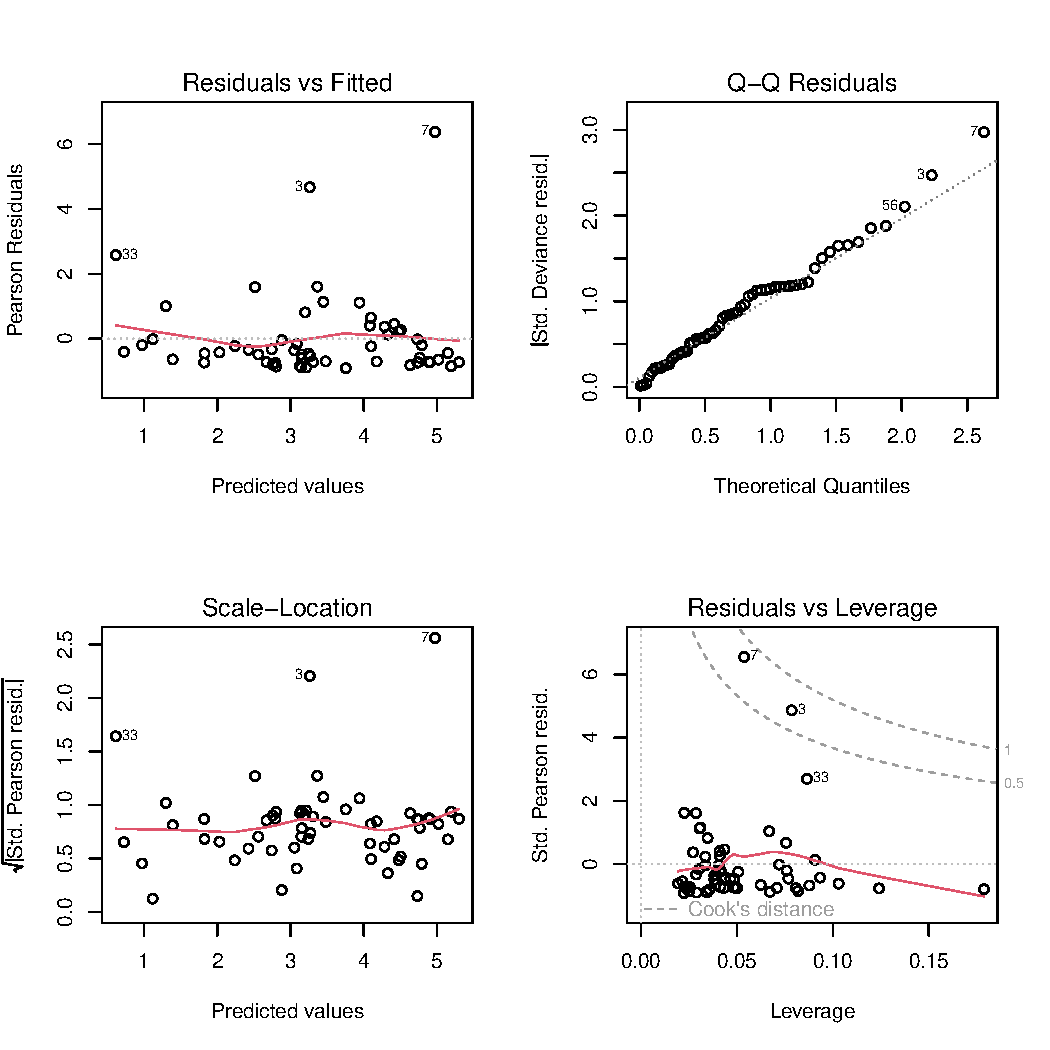
\includegraphics[width=\textwidth]{HelmBiogeog/Figures/ParDiv_diagnostics.pdf}
    \caption{Model diagnostics plots for our negative binomial model of \textbf{parasite richness} across islands, including residual vs fitted values (top left), Q-Q plot (top right), scale-location (bottom left), and residual vs leverage plot (bottom right), with dotted lines representing Cook's distance contours of 0.5 and 1, respectively. }
    \label{fig:parDivdiagnostics}
  \end{center}
\end{figure}

\begin{figure}[h!]
  \begin{center}
    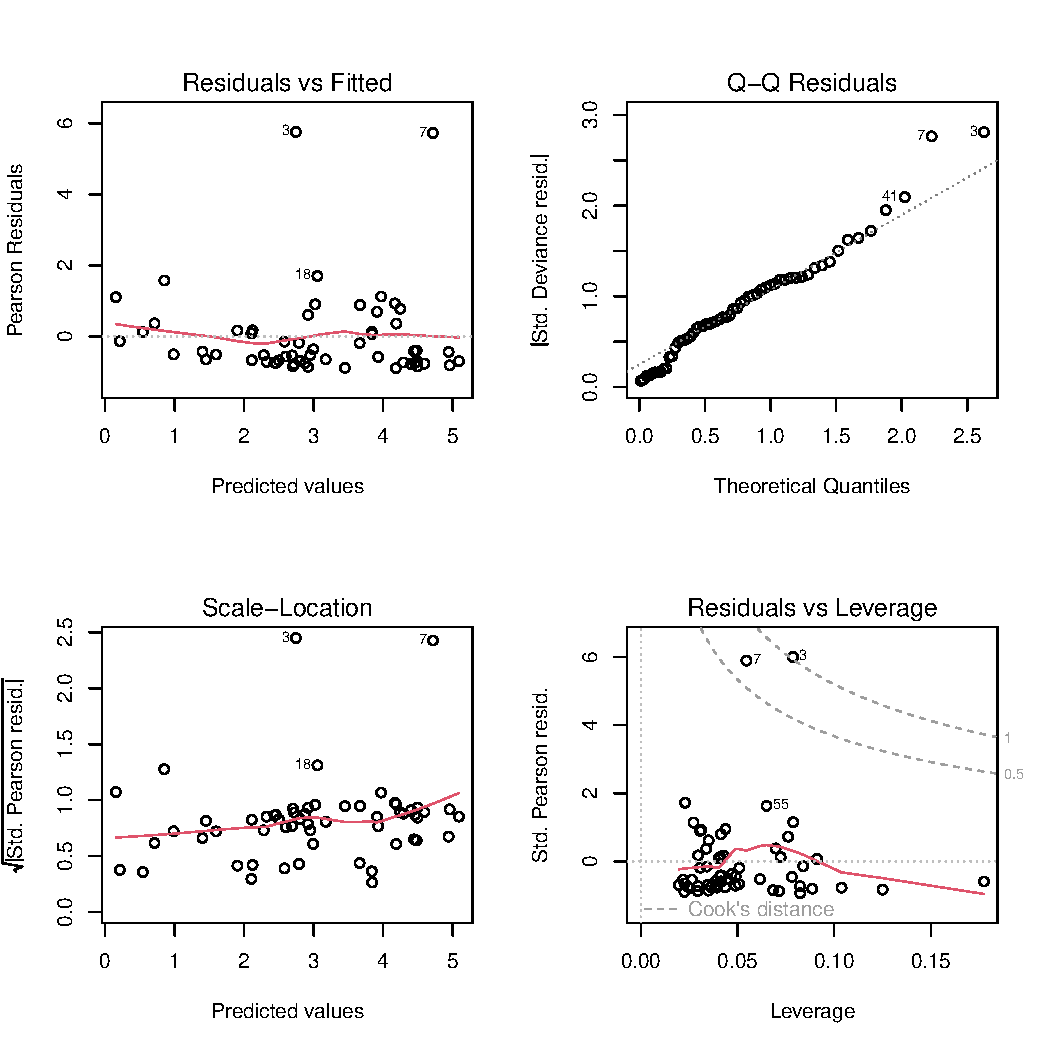
\includegraphics[width=\textwidth]{HelmBiogeog/Figures/HostDiv_diagnostics.pdf}
    \caption{Model diagnostics plots for our negative binomial model of \textbf{host richness} across islands, including residual vs fitted values (top left), Q-Q plot (top right), scale-location (bottom left), and residual vs leverage plot (bottom right), with dotted lines representing Cook's distance contours of 0.5 and 1, respectively. }
    \label{fig:hostDivdiagnostics}
  \end{center}
\end{figure}

\begin{figure}[h!]
  \begin{center}
    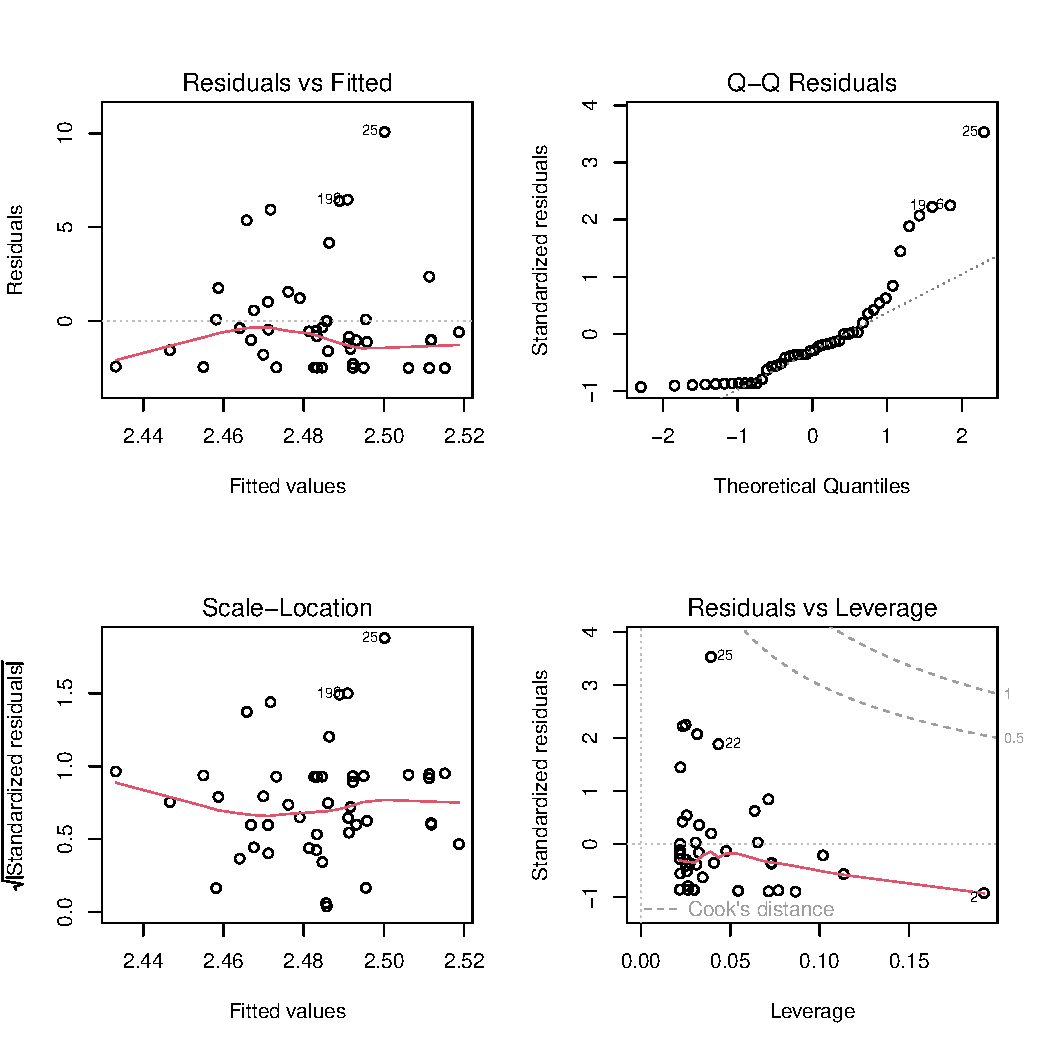
\includegraphics[width=\textwidth]{HelmBiogeog/Figures/NODFc_Distance_diagnostics.pdf}
    \caption{Model diagnostics plots for our generalized linear model of \textbf{network nestedness ($NODF_c$)} across islands, including residual vs fitted values (top left), Q-Q plot (top right), scale-location (bottom left), and residual vs leverage plot (bottom right), with dotted lines representing Cook's distance contours of 0.5 and 1, respectively. }
    \label{fig:nodfcdiagnostics}
  \end{center}
\end{figure}

\clearpage\\

\subsubsection*{The relationship between nestedness and modularity}

We don't consider modularity in the main text, but we explore it here for fun, as it is closely related to nestedness. Cite arxiv paper and Fortuna 2010 \citep{fortuna2010nestedness} and say that they are like...the same thing.


GF: How necessary do you think this addition is? Can add it back in if you think so, but would need to recalculate on our new network sets. 
\clearpage
                                                                  


\addtocontents{toc}{\protect\vskip-20pt}
\chapter[Structural Changes in Mutualistic Networks under Global Anthropogenic Pressure]{Structural Changes in Mutualistic Networks under Global Anthropogenic Pressure}   

\section*{\textbf{\underline{Abstract}}}
Plant-animal transport mutualisms, such as seed dispersal and pollination, represent a diverse suite of interactions that impact the function and dynamics of many ecological communities. Network representations of these interactions exhibit a wide range of structural properties (e.g. nestedness, modularity) that ultimately mediate emergent properties of ecological relevance (e.g. stability, resilience, robustness to secondary extinction). Understanding how these structural properties are affected by anthropogenic forcing and how they scale up to shape emergent properties is vital for predicting and conserving mutualistic networks in the face of global change. Here, I review the current state of knowledge on how three major classes of anthropogenic impact: shifts in global climate, land use intensification, and human-mediated invasion, affect the structural properties of plant-animal transport mutualism networks. In particular, I synthesize emerging patterns and persistent knowledge gaps in how these drivers alter network structure across systems and scales. Finally, I highlight a series of open questions in the field, the answers to which may help elucidate how these structural shifts scale up to changes in community dynamics, and ultimately improve our ability to predict and conserve mutualistic systems.

\section*{\textbf{\underline{Introduction}}}
\paragraph*{Mutualisms are important to the function of ecosystems}\mbox{}\\ 
The term "mutualism" covers a broad suite of species interactions, many of which are collectively vital to the function of many ecosystems as we currently know them \parencite{boucher1982ecology}, and iconic organismal features such as flowers or fruits are living homages to the mutualisms that they support \parencite{weiblen2015evolutionary}. The flow of resources facilitated by these and other mutualistic interactions can serve key ecological functions, and ultimately provide significant ecosystem services to human communities across the planet. Globally, pollinators may provide as much as \$400 billion annually in agricultural pollination services alone as of 2020 \parencite{porto2020pollination}, and are relied upon by 85\% of extant plant species across the globe \parencite{ollerton2011many}.
    

\paragraph{}
Due to their outsized impact on ecosystem function and services, understanding how mutualistic interactions change in response to perturbation is of great interest. These influential interactions do not happen in a vacuum, and taking a network approach to studying mutualisms can better allow us to understand how mutualisms as a whole affect the structure, function, and resultant services provided by an ecosystem. N	etwork approaches allow us to more clearly understand how perturbations propagate through a system, and have been used to study consumer-resource interactions \parencite{rooney2012integrating}, nutrient cycles, \parencite{christian1996nitrogen}, host-parasite interactions, \parencite{dallas2015co}, and mutualistic interactions \parencite{vanbergen2017network, rohr2014structural}. Together, these approaches have enhanced the ability to predict how diverse communities may respond to environmental change. In order to understand how communities of interacting species may change in the face of growing anthropogenic forcing, it is vital to understand how human-induced changes tend to affect the structure and function of mutualistic networks. 

%There have been massive changes in mutualistic networks
\paragraph*{}
Global ecosystems are subject to anthropogenically driven changes at increasing rates, and as a result, so are the mutualistic interaction networks that occur within them. Structural changes in mutualistic networks can be driven by a diverse set of drivers, including shifting climates, urbanization and land use changes, and invasion of non-native species. Here, I aim to characterize the current state of understanding about the ways these diverse drivers affect the structural properties of two major classes of plant-animal transportation mutualisms \parencite{bronsteinmutualism1}: seed dispersal and pollination networks, as well as how we can leverage our knowledge of these patterns to better understand, predict, and conserve these critical natural systems. 


% TD: you use 'we' 30 times. It's a bit informal to use this, but I also don't want to tell you to use the passive voice too much. Maybe change some of them, because I'm already picking up on it at this point and I think a reviewer will too. 

\paragraph*{Emergent Properties of Mutualist Networks}\mbox{}\\ 
The structure of relationships within mutualistic systems can generate dynamic system-level behavior, including several emergent properties useful for understanding how mutualistic systems may respond to perturbation (Figure \ref{fig:ConceptDraft}). These include properties describing how mutualistic networks behave around equilibrial states, a number of which can be estimated through eigenanalysis of the Jacobian matrix representing mutualistic communities at equilibrium. Both local stability (the tendency of the system to dampen small perturbations from equilibrium) \parencite{valdovinos2019mutualistic, okuyama2008network}, as well as resilience (here, the speed at which the system returns to equilibrium after perturbation) \parencite{thebault2010stability, suweis2013emergence}, are important for predicting how mutualistic networks respond to anthropogenic change. Other properties include the size of the feasibility domain, the range of parameter values that permits non-zero equilibrium abundances for all species in a community \parencite{saavedra2016nested, grilli2017feasibility, wang2023interspecific}. This property, sometimes referred to as structural stability, defines the safe operational space within which all species can persist \parencite{bascompte2022resilience}. Given an existing network structure, the extent to which disturbances spread widely or remain confined to local subsets of species \parencite{martins2024propagation, suweis2015effect} is yet another emergent feature of interest in the context of anthropogenic change, and is closely related to the structural property of modularity. 


\paragraph{}
These metrics collectively provide important insights into how existing network structure may mediate the impact of perturbation, but we are also interested in how networks may be sensitive to changes to their existing structure. By definition, mutualistic partners improve one another's fitness; if the magnitude of benefit scales in some way with population size \parencite{valdovinos2019mutualistic}, positive feedbacks between partnered populations or threshold responses \parencite{hale2021ecological} may occur. Disrupting these positive feedbacks of networks can facilitate critical transitions, and structural properties of networks can be important for determining behavior at the critical boundary or determining how robust a network is to loss of certain nodes or links \parencite{van2021facultative}. For example, simulated plant-pollinator networks with greater connectance are more likely to undergo large critical transitions as extinctions occur, undergoing larger community-level breakdowns instead of many small breakdowns \parencite{lever2014sudden}. Positive feedbacks may also induce hysteretic effects crossing the critical transition boundary; that is community assembly and disassembly processes may often be non-symmetric in mutualistic systems, with the outcome depending on precursor system states \parencite{cai2020mutualistic}. Understanding how these processes occur and are influenced by network structural properties is vital for both prediction and conservation of mutualistic systems.


\paragraph*{The Importance of Structural Properties}\mbox{}\\ 
%Structural features affect emergent ones
Many of these aforementioned emergent properties of interest (stability, resilience, hysteresis, etc.) are heavily impacted by network structural properties \parencite{landi2018complexity}. A significant body of existing literature has been devoted to interrogating relationships between the structural properties and emergent properties of species interaction networks, though at times with counterintuitive results. For example, network modularity (the property of having more connections within smaller subunits of a network than between them) tends to reduce the propagation of direct or indirect perturbations through a mutualistic system \parencite{thebault2010stability, okuyama2008network}. Invasion by non-native generalist species increases connectance and decreases modularity of some networks, potentially leading to broader or faster propagation of disturbances in the face of a changing environment \parencite{fricke2020accelerating, vollstadt2022plant, martins2024propagation}.  Because of their important and often complex effects on emergent properties, understanding how network structural properties tend to change in response to anthropogenic forcing is vital for prediction and management of mutualistic systems. 

%How structure -> Emergent is complicated
\paragraph*{} 
Structural properties often have nuanced effects on multiple emergent properties, making it important to identify which emergent properties are most relevant in a given context. For example, one widely observed property of mutualistic networks is nestedness, in which specialist species with few interaction partners tend to interact with generalist species that have many partners, effectively embedding specialist interactions within a broader, generalist core \parencite{bascompte2003nested, bascompte2006asymmetric, thebault2010stability}. As nestedness increases, the overall robustness of the system to species loss may increase due to functional redundancy, while simultaneously making the final breakdown of the system more dramatic (increasing magnitude of critical transitions) \parencite{bascompte2022resilience}. The nestedness of strong interactions tends to increase the size of a mutualistic system's feasibility domain \parencite{saavedra2016nested}, yet decrease its stability at equilibrium \parencite{allesina2012stability}. However, even if more nested mutualistic networks are less stable, they may lead to higher overall community abundance, an effect stronger in systems characterized by abundant but weak mutualisms \parencite{suweis2013emergence}. Robert May first pointed out in 1973 the ``paradox of complex interactions", where, under a Lotka-Volterra style modeling framework, larger species assemblages with many strong and randomly assigned species interactions lead to correspondingly smaller feasible domains of community stability \parencite{may1973stability}, a pattern that tends to be even more pronounced in mutualistic systems \parencite{allesina2012stability, saavedra2016nested}.  In reality, however, interactions are not randomly assigned within a community, and empirically observed suites of mutualistic interactions often tend to favor stability in practice, though to varying degrees \parencite{thebault2010stability, grilli2017feasibility}. How structural properties translate into emergent ones may be further complicated by plasticity in species interaction preferences \parencite{corro2021annual} or the degree of nodes' dependence on mutualisms \parencite{van2021facultative}. Valdovinos et al. (2016) found that accounting for potential adaptive foraging behaviors reversed the effects of nestedness and connectance on species persistence times \parencite{valdovinos2016niche}. In general, the relationship between structural and emergent properties is complicated and can lead to counterintuitive results \parencite{landi2018complexity}.

\paragraph*{} %How do structural features arise? 
The mechanisms under which emergent properties arise in networks across a landscape still warrant further investigation, especially in the context of mutualistic systems. In food webs, Borrelli et al. (2015) found that stabilizing motifs were overrepresented relative to null expectations across a diverse set of 50 networks, potentially indicating the presence of stabilizing processes present across landscape scales \parencite{borrelli2015selection}. This is supported by prior work looking at the constancy of network structural properties across scales in both trophic \parencite{fahimipour2014dynamics} and host-parasite \parencite{dallas2018compositional} networks, even as individual species turn over across space. The conservation of network properties despite species turnover may indicate that separate assembly mechanisms operate at the level of interaction networks and species assemblages per se \parencite{petanidou2008long, dupont2009spatio, burkle2011future, dehling2020similar, ten2024latitudinal}. One potential set of mechanisms acting on network structure may be non-Darwinian selection processes \parencite{saravia2022ecological}, where more stable networks endure longer through time as less stable networks break down, a potential phenomenon supported by theoretical modeling work \parencite{cai2020mutualistic}. However, one must be cautious in interpreting the prevalence of stabilizing structural properties as evidence for these processes; Saravia et al. (2022) found little difference between realized local networks and random draws from the regional metaweb in trophic networks \parencite{saravia2022ecological}, emphasizing the importance of proper null models in the context of network structure \parencite{maynard2018network, pellissier2018comparing}. Additionally, while different structural measures capture different aspects of network topology, they are seldom independent, a feature well-appreciated in food webs \parencite{vermaat2009major}. Understanding how structural properties covary is another reason null model approaches are important and looking at joint properties may be useful \parencite{fortuna2010nestedness, poisot2014ecological, pellissier2018comparing, dormann2017}. 



%Network properties may also influence individual species fitness components predictably, according to their traits, with even the fitness benefit conveyed by given interactions depending on community structure (ex. Specialists in nested communities had higher closeness centrality. 



\paragraph*{Widely Observed Structural Properties of Mutualistic Networks}\mbox{}\\ 
%Emp Nets are Nested
There are a number of properties pervasive in empirically observed frugivory and floral visitation networks. Empirical networks often exhibit high degrees of interaction nestedness \parencite{fortuna2006habitat, bascompte2006asymmetric}, a product of the asymmetric specialization widely observed in both seed-dispersal \parencite{yohe2025frugivore, schleuning2014loss} and floral visitor networks \parencite{bascompte2003nested}. This feature tends to increase the strength of highly connected nodes, often resulting in long-tailed degree distributions. Especially in pollination systems there may be trade-offs in specialization stemming from this pervasive interaction asymmetry; \parencite{arceo2020plant} found that a plant's degree specialism was positively related to heterospecific pollen delivery, likely due to associations with generalist pollinators \parencite{arceo2020plant}. Nestedness may increase positive indirect interactions within guilds, ultimately increasing the potential diversity of species a community can support \parencite{bascompte2003nested, guimaraes2017indirect}. It also can reduce effective interspecific competition, increasing equilibrial species richness \parencite{bastolla2009architecture}, a pattern potentially observed in empirical networks \parencite{Gonzales2015macroecology}. 

%Emp Nets are Modular
\paragraph*{}
Modularity is another prevalent feature of mutualistic networks, many of which may be separated by functional guilds \parencite{ramos2018modularity} or phylogenetically conserved groups of interaction partners \parencite{Gonzales2015macroecology}. Species with certain traits or within certain taxonomic groups may be more likely to make cross-module connections. Sebasti{\'a}n-Gonz{\'a}lez (2017) found that a small number of highly frugivorous birds and high energy content fruits had higher connectivity both between and within modules \parencite{sebastian2017drivers}. In their study of Peruvian highland pollination networks, Watts et al. (2016) found connector species were likely to be comparatively generalist and taxonomically clustered (\textit{Diptera: Syrphidae} and \textit{Asterales: Asteraceae}). The introduction of a relatively small number of species with higher or lower propensity to establish cross-module connections can fundamentally alter the resultant modularity of a given network \parencite{russo2014patterns}, an idea further explored in the section \textbf{Invasion}.  
%Emp Nets are Sparse? Do I need to talk about this? Ecological networks are generally sparse, a feature that can be a problem for prediction. 
% TD: eh. If the focus was on prediction, I would say sure, but 1 sentence tops should be spent on that, and I'd do it in a section where you talk about how lower-level properties scale to emergent properties (i.e., sparse networks can't really be nested, right?). 


%Emp features may change across space...
\paragraph*{}
Agnostic to changing environments, some evidence shows that network structural properties vary across preexisting environmental or spatial gradients.  In a study of both insect and avian pollination networks across broad latitudinal coverage  Tr{\o}jelsgaard and Olsen (2013) found that modularity was highest at low latitudes whereas nestedness peaked at mid-latitudes \parencite{trojelsgaard2013macroecology}. Across altitudinal gradients, multiple studies have observed an increase in phylogenetic generalism and an associated increase in nestedness and connectance with increasing elevation in plant-pollinator networks \parencite{adedoja2018insect, lara2019beta, classen2020specialization}, though similar evaluations to my knowledge have not been made in frugivory systems. 

%Or climate.
\paragraph*{}
Both the mean and variability of temperature may also play a role in shaping network structural properties; Welti et al. (2015) found that both seed dispersal and floral visitation networks were generally more nested in areas with higher inter-annual temperature variability \parencite{welti2015structure}. Gonz{\'a}lez et al. (2015) found that in mainland plant-hummingbird networks warmer and more stable climates were associated with higher modularity, though these variables had no effect on island networks \parencite{Gonzales2015macroecology}. Both current and past climatic features may have significant effects on network structure \parencite{dalsgaard2013}, further complicating the question of how and at what rate networks may respond to future climatic change. 

\section*{\textbf{\underline{Anthropogenic Change and Mutualistic Network Structure}}}
%Transisition into three drivers sections
While existing environmental conditions have already played a role in shaping mutualistic networks as we know them, human impacts have also drastically altered biotic and abiotic conditions across most of the globe. As natural ecosystems are subject to increasingly severe anthropogenic impacts, so too are the ecological networks that occur within them. Understanding how human-mediated changes affect structural properties and resultant dynamics of mutualistic networks is vital for predicting and conserving species interactions. These changes can occur through several mechanisms, including (1) alterations in community composition, (2) shifts in the probability of interactions occurring, and (3) disruptions to the coevolutionary processes underpinning these networks \parencite{tylianakis2017}. Here, I focus on how three major types of anthropogenic disturbance—climatic shifts, changes in land use, and human-facilitated invasion by non-native species—act through these mechanisms to reshape the structural properties of natural mutualistic networks.
\paragraph*{Climate}\mbox{}\\
Changes in climate can affect mutualistic network structure through a number of mechanisms, including inducing changes in species distributions across time and space, altering species abundances, or altering the physiology of interacting organisms. Many plant-animal mutualisms may only be able to occur during relatively short, yet ecologically important developmental or life history windows. For example, animal pollination can only occur when both the flowering time of the plant and the seasonal activity period of the animal intersect. As climate shifts the timing of these developmental periods, phenological shifts and subsequent mismatches have the potential to occur, altering the strength of mutualistic interactions or even removing them altogether \parencite{zettlemoyer2019phenology, burkle2013plant, teixido2022anthropogenic} . For example, in a forest-prairie floral visitation network Memmott et al. (2007) showed that up to 50\% of floral visitors have reduced overlap between their seasonal activity period and known floral resources over the past century \parencite{memmott2007global}. Link rewiring, in which species form new linkages in response to environmental change, may help alleviate some of the effects of phenological mismatch, but fitness reductions due to reduced phenological overlap with mutualists have been observed empirically \parencite{kudo2019spring, de2023warming}. Corresponding reduction in pollinator fitness have yet to be observed in field systems, though these reductions are likely already occurring in some contexts \parencite{gerard2020global}. These altered interaction probabilities can scale up into altered network structural properties; Encinas-Viso et al. (2012) found in simulated communities that increasing phenological overlap between competitors led to less stable, less nested, and ultimately less speciose communities \parencite{encinas2012phenology}. As climate shifts phenological periods, even if mutualistic interactors remain phenologically coupled, intraguild shifts in species' activity periods (such as overlapping flight or flowering periods) can change competitive interactions with cascading effects through the community \parencite{wang2023interspecific}.
    %Spatial mismatch
    \paragraph*{} 
    Even if mutualistic partners do not become decoupled in time, climate-driven range shifts may also decouple partnerships by reducing spatial overlap. Warming conditions may shift species ranges northward latitudinally or higher in elevation. Differences in features such as generation time and dispersal capacity mean that two mutualistic partners are unlikely to be able to shift their distributions at the same rate. Or, if biotic interactions limit the distributions of some mutualistic species, partners may be unable to shift ranges without commensurate shifts of the distributions of their partners \parencite{warren2014mutualism}. This may be especially salient in the case of seed-dispersal mutualisms, where the ability of plant species to shift their ranges in response to climatic changes may be dependent on their interaction partner \parencite{warren2014mutualism}.

    \paragraph*{}
    While species may shift their distributions or phenology to track preferred environmental conditions, climate change can also alter species abundances, potentially leading to local extirpation. Complete extirpation is not necessary for ecological disruption, however; functional extinction can precede or occur independently of true extirpation when populations become too small to effectively fulfill their roles as mutualists \parencite{costa2018defaunation}. Moreover, mutualistic partners often differ dramatically in their adaptive capacity due to contrasting life histories, such as generation time and population size \parencite{toby2010mutualisms}. For example, the adaptive potential of semelparous insects with annual life cycles differs substantially from that of the long-lived plants they pollinate. Existing work has already shown plant-animal mutualisms are generally weakened by climate change across broad scales \parencite{tylianakis2008global}. Climate-driven extinctions are not necessarily random, and taxonomic or functional biases in abundance changes may have large effects on network properties. Schleuning et al. (2016) found that higher elevation montane mutualism networks were less robust to climate-mediated losses than their lower-elevation counterparts \parencite{schleuning2016ecological}. Limitations to upslope movement have already been shown to reduce population size or extirpate montane species \parencite{freeman2018climate}, potentially putting high elevation mutualistic networks at higher risk of network breakdown. 
    
    %Changes to the phisiology of interactions
    \paragraph*{}
    Changes in environmental conditions may also alter the strength of a given interaction through changes in physiology or interaction preference \parencite{cruz2023mutualisms}, potentially leading to interaction breakdown. Hoover et al. (2012) observed shifts in nectar chemistry as a function of altered pCO$_2$, warming, and nitrogen deposition, which then had downstream effects on experimental pollinator preference and longevity \parencite{hoover2012warming}. Similar changes in pollen quality may also affect nutritional rewards of interactions, altering the fitness or preference of plants or pollinators \parencite{gerard2020global}. These sorts of processes may alter the coevolutionary processes underpinning the development of mutualistic networks, or cause negative fitness consequences in taxa without the plasticity to alter their interaction patterns accordingly. Warming conditions also tend to reduce body size in insects while exerting less predictable effects on the size of plants; this could potentially alter matching of specialized insect feeding morphologies with their plants \parencite{gerard2020global}. These sorts of mismatches can degrade interactions as a function of environment, and understanding how both plant and pollinator traits might shift with changing environments is important for predicting the outcomes even for contemporary interactions \parencite{cruz2023mutualisms}.
    
\paragraph*{Land use}\mbox{}\\
Human-mediated changes in land cover result in large shifts in habitat availability, both in absolute area and spatial distribution. At local scales, the impact of land-use change on network structure depends on the speed, type, and extent of conversion. For example, Theodorou et al. (2017) found previously agricultural areas actually increased in both floral and bee diversity when urbanized, emphasizing the importance of establishing useful bases of comparison \parencite{theodorou2017structure}. As natural areas are fragmented, specialized and rare interactions are lost disproportionally \parencite{aizen2012specialization}, with remaining generalist interactions potentially forming a widespread consistent core of interactions at landscape scales. This loss can be driven by the actual extirpation of specialists from the community itself \parencite{maurer2024landscape}, or by shifting biotic or abiotic contexts reducing the prevalence or efficacy of those interactions \parencite{birkenbach2024land}. In the case of habitat fragmentation, even if overall habitat loss is small the proportion of edge area is increased as existing land-cover types are subdivided. As edge-habitats become more prevalent across the landscape, networks may grow increasingly homogenized as turnover decreases over larger spatial extents, even if local assemblages retain their diversity or structure. 

    
    \paragraph{}
    While land-cover conversion can often have profound impacts on the presence of individual species or interactions at a given site \parencite{theodorou2017structure, schneiberg2020urbanization, maurer2024landscape, birkenbach2024land}, whether these changes scale up into differences in overall network structure may be more context-dependent. For example, a recent paper by Rossi et al. (2025) quantified changes in frugivore networks in disturbed Amazon forest plots, finding that while logging and burning across timescales did reduce richness of both interacting species and links between them, neither had predictable impacts on network structural properties \parencite{rossi2025anthropogenic}. Salazar-Rivera et al. (2020) found that modularity was maintained in periurban frugivory networks compared to undisturbed habitats, only observing a decrease in nestedness  \parencite{salazar2020frugivory}. Network properties at local scales may be maintained if land use changes exert too small of an impact on structural or functional properties of mutualistic assemblages to cause appreciable changes in network structure. However, a lack of difference across disturbance regimes may also be an indication of comparatively strong constraints on potential structural properties that can be realized in a network comprised of a given regional pool of mutualists. 
    
    \paragraph{}
    Observed network structures may help mutualistic communities deal with disturbance, or at least mediate their responses. Fortuna and Bascompte (2006) found that empirically observed networks were more sensitive to simulated small reductions in habitat area, but persisted longer than randomly assembled graphs in the face of severe disturbance, largely due to the large amount of nestedness observed within empirical networks providing functional redundancy \parencite{fortuna2006habitat}. Further empirical observations of how structural properties both mediate the response of mutualistic networks to change, as well as how these changes feed back to alter structural properties are warranted. Even if structural properties are not negatively impacted by altered land use, specific ecosystem services may still be disrupted \parencite{menke2012plant}. For example, Menke et al. (2012) found that frugivory networks along forest edges were more nested and had greater connectance,  but saw an overall decrease in dispersal of large-fruited forest-specialist plants \parencite{menke2012plant}. While helpful for predicting and understanding changes in mutualistic networks, relying on structural properties alone as indicators of network change can mask functionally critical losses. In practice, isolating the effects of land use change from other anthropogenic drivers is often difficult. Areas with large amounts of human-mediated land cover conversion are often subject to increased propagule pressure of nonnative mutualists \parencite{liu2023impact}, which may have their own impacts on network structural properties. 









\paragraph*{Invasion}\mbox{}\\
Human-mediated dispersal has vastly altered species distributions across the globe, and patterns of non-native species invasion can have persistent effects on the structural properties of mutualistic networks. Species with generalist interaction strategies can more easily invade existing ecological networks \parencite{piechnik2008food} and species roles are often conserved between native and invaded ranges \parencite{emer2016species}. Invasive plants are often effectively dispersed by generalist pollinators and seed dispersers \parencite{richardson2000plant}, though in general many successful invaders can also successfully interact with relative specialists in their new range \parencite{stouffer2014exotic}. How the traits of a potential invader relate to the existing community can affect its propensity for invasion; in simulated communities Minoarivelo and Hui (2016) found potential invaders with trait means different from the existing community were more likely to successfully establish \parencite{minoarivelo2016invading}. The generalism or specialism of a potential invader may also be predictive of its effect on network properties given establishment \parencite{russo2014patterns}.

    \paragraph{} %homogenation across scales
    As synanthropic generalist species are introduced into more human-affected habitats, mutualistic assemblages and potentially network structures tend to homogenize across regional scales \parencite{fricke2020accelerating}. Even when homogenization across space is limited in the context of the entire community, persistent "invader complexes" of introduced species that interact with each other may still alter network properties or invasibility \parencite{richardson2000plant, prior2015mutualism, vollstadt2022plant}. Generalist invaders may also have hysteretic effects on networks once well integrated into existing assemblages. In networks where invasive plants have already established, removing them may in fact further alter network structural properties than allowing them to persist \parencite{valdovinos2009structure, aslan2019implications}. Reliance on non-native pollination partners may further exacerbate the effects of other anthropogenic disturbances. Zettlemoyer et al. (2019) found higher phenotypic plasticity and greater phenological shifts in introduced plant species compared to native taxa, potentially further increasing the risk of phenological mismatch between native pollinators and introduced plants they now rely on \parencite{zettlemoyer2019phenology}. Alternatively, while introduced mutualists may provide some direct benefit to native partners, their net effect may remain negative when indirect impacts are considered \parencite{vidal2021variable}. If invading species exert competitive pressure that reduces the abundance of their native intraguild counterparts while simultaneously being less effective at fulfilling mutualistic functions (pollination, protection, etc.), mutualistic networks may collapse functionally even as interactions (e.g. floral visitation, etc.) appear to continue. While tight coevolutionary coupling is seen between some specialist partners \parencite{stebbins1970adaptive}, the widespread generalism exhibited in many animal-plant networks can cause indirect impacts of invaders to play a large role in shaping their eco-evolutionary trajectories \parencite{guimaraes2017indirect, medeiros2018geographic}. Native preferences to associate with introduced mutualists could even cause invasional meltdown of native interactions, a phenomenon exemplified in avian frugivory networks in Hawaii \parencite{VizentinBugoni2021}.


    \paragraph{} %Invasion of generalists leads us to expect changes in invaded network properties, though evidence is mixed in practice 
    If invasion favors generalist species \parencite{piechnik2008food, fricke2020accelerating}, one might expect directional changes in network properties associated with widespread invasion, especially if coupled declines in native mutualists or shifts in their interaction patterns \parencite{aizen2008invasive}. Supergeneralist invaders may significantly increase nestedness by creating cross-module connections \parencite{traveset2014mutualistic}, allowing perturbations to propagate through the network farther and with greater strength. However, invasive species may also provide functional redundancy of potential partners, potentially buffering mutualistic networks against species extinction. Such buffering may not always translate to greater robustness or resilience in the face of broader perturbations. 
    
    \paragraph{}
    In addition to structural properties, emergent properties such as robustness or resilience may be important for predicting the invasibility of a given network \parencite{minoarivelo2016invading}. The presence of invasive mutualists can modify how networks respond to perturbation, potentially altering the severity or likelihood of coextinction cascades. By simulating secondary extinction cascades in invaded or uninvaded empirical networks, Vanbergen et al. (2017) found that coextinctions were less likely in disturbed networks due to functional redundancy of partners \parencite{vanbergen2017network}. However, given that an initial coextinction event occurred, the risk of a cascading collapse was actually higher in these networks, highlighting how expectations about how invasion may impact short- and long-term responses to change differently in some scenarios. 
    
    \paragraph{}
    Expectations for how structural properties translate into emergent properties may be very different depending on the strength and structure of competition within the community \parencite{pascual2017mutualism, wang2023interspecific}. In addition to global homogenization of interactions across scales, Fricke and Svenning (2020) found that more highly-invaded frugivory networks had higher connectance and lower modularity \parencite{fricke2020accelerating}. Some evidence exists that the increasing prevalence of synanthropic generalists in some pollinator communities increases interaction evenness \parencite{schneiberg2020urbanization} or nestedness \parencite{bartomeus2008contrasting}, though the exact pattern of this may depend on factors such as pollination syndrome or local pollinator communities. Vanbergen et al. (2017) also found that disturbed pollination networks were larger, but actually lower in connectance and nestedness \parencite{vanbergen2017network}. Even further complicating expectations, numerous other studies have also observed little to no predictable impact of invasion on overall network properties such as nestedness or modularity \parencite{stouffer2014exotic, parra2021impacts}, even when considering invasion of hypergeneralist plant species \parencite{vila2009invasive}. Further investigation into the processes maintaining network properties despite significant node-level changes is needed to fully synthesize these variable results across systems. 

\section*{\textbf{\underline{Additional Considerations}}}
\paragraph*{The Role of Rewiring}\mbox{}\\
Ecological networks are not static through time or space. While links between species may erode through time in response to changing environments, new links may form as well, a process known as link rewiring. This phenomenon is an important consideration when assessing how mutualistic networks may respond to anthropogenic pressures. While it remains essential to account for processes that erode existing interactions (e.g., phenological mismatches, species extinctions, etc.), failing to account for potential rewiring may lead us to overestimate their effects \parencite{vizentin2020including}. However, despite recent conceptual advances in understanding the rules and constraints that govern rewiring \parencite{corlett2011frugivore, fuzessy2024navigating}, in practice it is often unclear how networks will rewire until they are perturbed, and they may at times fail to rewire as strongly as expected \parencite{leimberger2023plant}. Leveraging predictive approaches can be potentially powerful in this context in order to better understand how networks may respond to change \parencite{eklof2013dimensionality, vizentin2020including, strydom2021roadmap, strydom2023graph, nunes2024estimated}, but to date there are relatively few case studies looking at how networks change through time (though see \parencite{burkle2013plant, olesen2011strong, leimberger2023plant, petanidou2008long}). This gap has been long-acknowledged in the literature \parencite{bascompte2007plant}, but due to the logistical challenges and significant resource requirements of resampling interactions at a given site regularly it is one that we have been slow to fill as a scientific community. From the evidence that does exist, species traits or position within a network may be predictive of their persistence \parencite{burkle2013plant} or rewiring \parencite{sandor2024spatial}.

\paragraph{}
In some cases, phylogenetic conservation of traits or interaction preference may be useful for determining which species may be interacting in present assemblages, as well as which interactions may occur between novel sets of species. This approach has been applied in modern systems \parencite{VizentinBugoni2021} and used to gain insight into paleoecological systems of interacting mutualists \parencite{Braga21}. In other systems, however, phylogenetic relatedness may explain less variation in interactions than directly measured traits \parencite{rafferty2013}. Machine learning approaches can help overcome the problem of predicting potential species interactions as well as potentially identify traits associated with rewiring potential \parencite{pichler2020machine, foster2026comparing}, though care needs to be taken in applying many of these approaches to notoriously sparse ecological data \parencite{poisot2023guidelines}.

\paragraph{}
Species' capacity to rewire may be an otherwise hidden or underappreciated potential of functional redundancy, and affinity-based rewiring has been shown to maintain network properties and stability in theoretical systems \parencite{sheykhali2020robustness}. There are also new exciting avenues for measuring the rate and scale of rewiring as well, with potential for application in ecological systems \parencite{han2019measuring}. However, it is also important to emphasize that mutualistic interactions are not the only relationships being affected by global change. Competitive and trophic interactions are also likely to be affected by anthropogenic drivers, potentially complicating the picture of the emergent outcomes of rewiring. Furthermore, shifts in environmentally-mediated interaction strengths can fundamentally alter the dynamics of a network, even without changing its overall structure.  Mechanisms to maintain mutualisms may be developed on coevolutionary timescales, and species may not be able to alter interaction patterns to reflect current fitness benefits \parencite{toby2010mutualisms}. However, this is not always true; flexibility in interaction preferences has been observed across numerous pollinator \parencite{moran2022flexible} and frugivore taxa \parencite{nowak2013specialist}, and adaptive foraging may help ameliorate the negative impacts of environmental change in some animal taxa \parencite{valdovinos2016niche}. 

% TD: damn this is a long section that seems almost tangential to the main thesis/point of the review. Maybe it's not. 



\paragraph*{The inherent issue of sampling}\mbox{}\\
Network representations can be useful tools for studying ecological systems, but sampling and model-construction choices can introduce artifacts into inference \parencite{bluthgen2024critical, olesen2011missing, Young21}. Sampling capacity and efficacy varies widely across different types of mutualistic systems, and biases may potentially lead to artificial structural properties. For example, at least some of the persistence of patterns of high nestedness and low connectivity of many ecological networks may be a byproduct of poorly sampling them \parencite{bluthgen2024critical, bluthgen2008} or neutral evolutionary processes \parencite{Valverde2018}. One solution to circumvent this shortfall is by combining data from multiple sources \parencite{olesen2011missing, cirtwill2019quantitative}, such as independent abundance estimates or alternative sources of interaction data. By properly combining data from multiple sources it becomes possible to account for these structural artifacts as well as characterize higher-order interactions and structure, even without a fully sampled network \parencite{valdovinos2019mutualistic}. 



\paragraph*{}
When describing or characterizing networks, the scale of aggregation chosen should be biologically motivated. Combining data across too large a spatial or temporal extent can artificially decrease network connectance and lead to misinterpretations regarding species generalism or network turnover \parencite{burkle2011future, duchenne2022seasonal}. As potential partners that never co-occur in time or space are aggregated into the same network, this creates an overabundance of "missing" links. As such, the same network may exhibit different structural properties depending on the level of aggregation \parencite{guimaraes2020structure}. Species considered generalists across their range may function as relative specialists at individual sites, with local populations only interacting with a narrow handful of partners in any given biotic context. Eco-evolutionary modeling \parencite{medeiros2018geographic} found that gene flow among generalist populations may actually increase their trait-matching to local mutualists. Even in the same habitats, network properties may change across fine scales (e.g. forest floor to canopy) \parencite{schleuning2011specialization}. While network approaches necessarily simplify complex ecological systems, methodological choices can substantially influence the structural properties observed and the conclusions drawn from them.

\paragraph*{}
Additionally, many theoretical expectations for how structural properties translate into emergent properties rely on simulating truly mutualistic networks, where interactions between mutualists by definition confer a positive fitness benefit to both interacting species. However, interactions may not always convey a fitness benefit in practice \parencite{thomson2003mutualism}. The fitness impacts of opportunistic interactions, "cheaters", palynivory, and granivory are often difficult to quantify, especially as the interaction is often contributing to fitness of each partner in very different ways (e.g. the benefit of resource for a pollinator is difficult to measure against the fitness benefit of pollination for a plant). ``True" mutualisms -- where both organisms receive a positive fitness benefit -- may actually be more conserved than interaction networks show \parencite{burkle2011future, montesinos2017network}. Additionally, even the fitness effects of existing interactions may shift along the mutualism-antagonism continuum as climate alters the cost-benefit relationship of an interaction \parencite{toby2010mutualisms}. Empirically measuring the fitness effect conveyed by an interaction is logistically challenging but vital work, especially in the context of global change. There is some evidence, at least in pollination systems, that easier to measure properties such as interaction frequency can be a useful surrogate for fitness benefit \parencite{vazquez2005interaction}. However, it remains unclear whether this relationship holds across broader spatial scales or applies to other forms of transport mutualism.


\paragraph*{Network approaches for conservation planning and assessment}\mbox{}\\ 
The idea of conserving species interactions has been around for nearly a half-century \parencite{Janzen1974Deflowering}. Conserving mutualist assemblages and reducing the rate of anthropogenic impacts can help mitigate potential future degradation of existing networks, but a large amount of change has already occurred in many mutualistic systems. Accounting for both existing and potential future changes during conservation planning and assessment is a vital reality for effective management of ecosystems. Clear links between management goals and measurable outcomes are also essential in network contexts. For example, practices allowing or promoting temporal variance in population size across a community generally have positive effects on network stability \parencite{bascompte2022resilience}, but may be counter to management practice for individual species \parencite{tylianakis2010conservation}. 

\paragraph*{}
While conceptually linked, not all transport mutualisms are equal. Plant-pollinator relationships require an individual pollinator to engage in multiple interactions with the same species for successful conspecific pollen transfer, whereas effective seed dispersal can occur as the result of a single frugivory interaction. The different fitness benefits and mechanisms of these interactions may translate into very different impacts of global change on their structure and coevolutionary underpinnings \parencite{wheelwright1982seed}. Regardless, taking network-level approaches to ecological questions can provide insight into numerous foundational ecological properties, and understanding how networks change may have relevance in the community beyond the confines of the network itself \parencite{windsor2022using}.

%-----------------------
\section*{\textbf{\underline{Conclusions}}}

Mutualistic networks represent complex webs of interactions that underlie essential ecosystems. Here, we have reviewed evidence that ever-increasing human impacts inflict non-random changes in the structural properties of these networks, which have the potential to scale up into emergent properties of ecological and evolutionary consequence. Anthropogenic shifts in global climate, land use, and species assemblages all have the potential to alter mutualist assemblages and the interactions between them. Understanding how resultant changes in the structural properties of mutualistic networks influence community dynamics can allow us to better predict how networks may respond to future perturbations, but additional research is needed to highlight the mechanistic causes and consequences of these changes. Across all three types of anthropogenic impacts discussed, there are examples of relatively drastic changes in node or interaction-level properties failing to scale up into expected changes in structural or emergent properties of networks. Further investigation of the rules that govern how these interactions scale up to network-level properties, especially in the context of empirically disturbed networks, is warranted. 

\paragraph*{}
In many ways, theoretical advancements in our ability to predict how networks may respond to environmental change have outpaced empirical evaluation of these predictions. Sampling a given network repeatedly through time is labor intensive, but a vital effort necessary to begin closing this gap. Existing empirical work looking at network change through time has made vital steps forward in our understanding of how mutualistic networks change throughout time. Non-Darwinian selection processes \parencite{borrelli2015selection, saravia2022ecological}, in which more stable network structures persist longer through time as less stable networks break down, have been predicted theoretically \parencite{cai2020mutualistic}, but empirical investigation of this phenomenon in mutualistic systems remains limited. Clarifying the extent to which stabilizing dynamics operate at the network level and identifying appropriate null models for comparison remains an important area for future investigation.

\paragraph*{}
Structural properties can be powerful for understanding how species interaction networks may respond to global change, but not if we lack a coherent understanding of how structural properties scale up to ecologically meaningful outcomes. Many existing structural metrics applied to ecological networks are borrowed from analysis of non-ecological graphs. Moving beyond single-metric summaries towards approaches that characterize the distribution, covariance, and constraints among multiple node, interaction, and network-level properties may provide a more complete picture of the operational space these networks may occupy. A deeper understanding of the relationship among structural properties, and between structure and function in mutualistic communities, will be essential for revealing the principles that govern network responses to global change. 

\paragraph*{}
These questions are especially urgent in the face of accelerating anthropogenic change. As climates shift, land-cover changes, and species introductions rewire ecological communities, the persistence of mutualistic networks will depend on their capacity to reorganize in response. Identifying which structural properties matter, under which contexts, and for which outcomes, remains an essential need in the context of a changing world. Repeated, interannual sampling of mutualistic networks as they respond to shifting environments is especially important for bridging the gap between theoretical predictions and empirical models of network change. With a proper understanding of these processes, we may be able to move from simply describing how networks change in response to perturbations to actively managing them in ways that help them endure. 

% TD: a bit of a conservation focus in the conclusions (and a bit throughout). That's fine (unless reviewers take issue). There's no outlining of open questions, which could be a good addition to try to target and motivate future research, while also acknowledging that the 'call to action' in the paragraphs above don't capture the full space of what should be done (if this makes sense). I'd probably read the last 3-4 paragraphs of that styndom paper to see what their 'call' looks like. Or one of the other reviews like Tylianakis. Otherwise it reads as pretty solid, and may get accepted through the amount of work surveying the literature while maybe not offering as strong of a synthetic bit as other reviews would have. 

\section*{\textbf{\underline{Outstanding questions}}}

\begin{enumerate}
    \item How does the relationship between structural and emergent properties change depending on the temporal or spatial scale of aggregation? Does choosing too broad or narrow a spatial scale obscure the impacts of structural properties on network dynamics? 
    \item How can considering distributions of node or interaction level traits alongside network structural properties improve our understanding or prediction of emergent properties? 
    \item Network structural properties inherently covary \parencite{poisot2014ecological, pellissier2018comparing}. Can we leverage our understanding of how these properties constrain one another to more effectively predict emergent network properties from suites of structural metrics, rather than from individual properties alone?
    \item How is the feasibility domain of a given network \parencite{bascompte2022resilience} constrained by the underlying species pool and suite of possible interactions? Can we use characterizations of this space to better understand how mutualistic systems may respond to future anthropogenic change? 
    \item Does "non-Darwinian selection" \parencite{borrelli2015selection, saravia2022ecological} on stabilizing properties play a role in maintaining mutualistic network structures over eco-evolutionary timescales? If so, when might these processes maintain mutualistic function in the face of changing environments? 
    \item Most existing work on the stability of mutualistic network structures has focused on static network properties; how might selection towards stabilizing properties influence sequential assembly processes? 
    \item Why do substantial changes in species or interaction-level properties so often fail to translate into measurable changes in overall network structure, and what does this reveal about the processes that maintain structural stability in mutualistic systems?
    \item How can insights gained from characterizing network structural properties be translated into actionable conservation and management strategies?
\end{enumerate}

\clearpage
\section*{\textbf{\underline{Figures}}}

\begin{figure}[h!]
  \begin{center}
    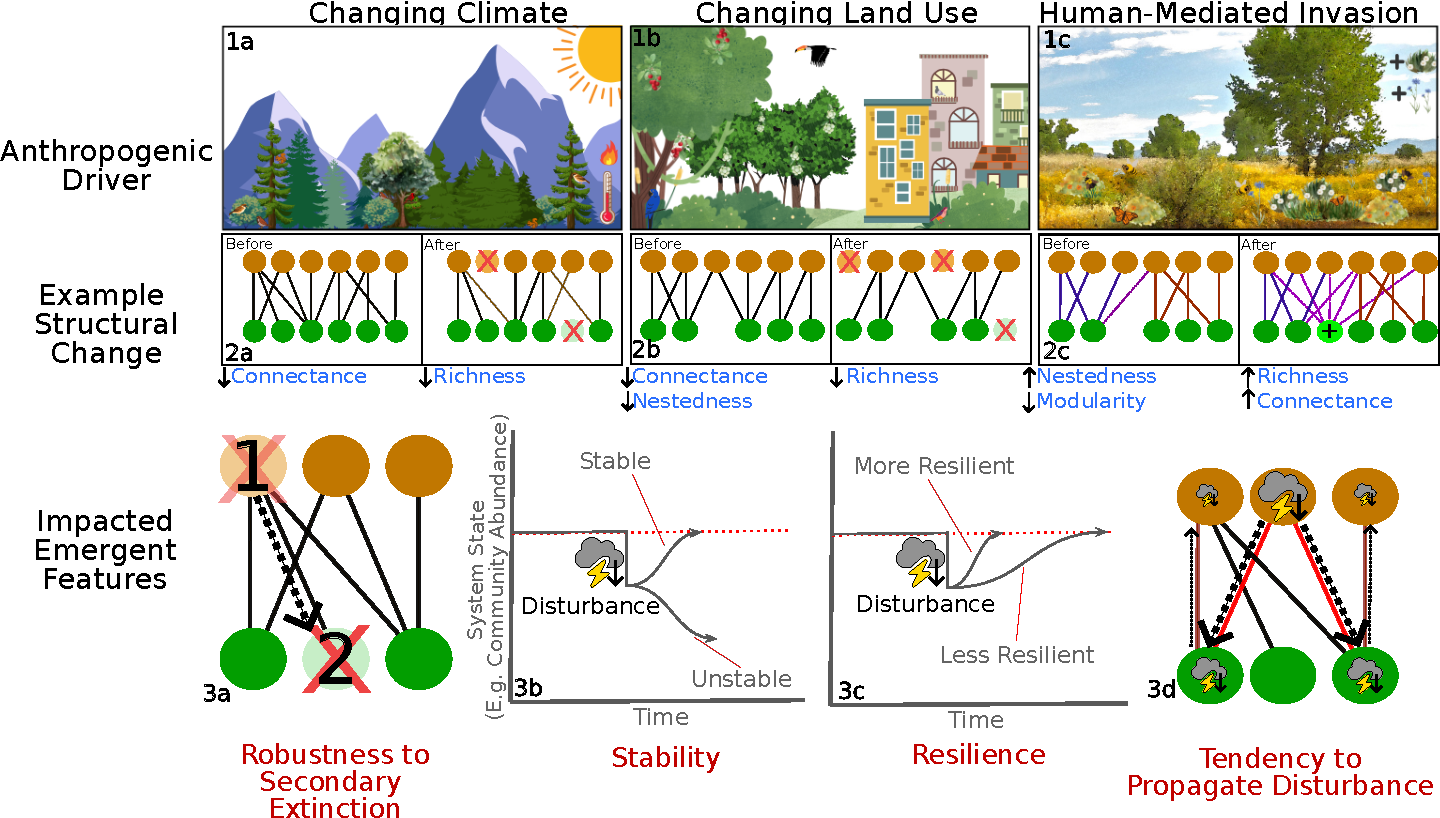
\includegraphics[width=\textwidth, alt={Graphic illustrating anthropogenic drivers of structural changes in animal-plant transport networks. The top row visualizes three main drivers, changing climate, changing land use, and human-mediated invasion, while visualizing potential network impacts. The graphic also visualized potentially impacted emergent properties of networks, including robustness to secondary extinction, stability, resilience, and tendency to propagate disturbance.}]{Review/Figures/ReviewConcept.pdf}
    \label{fig:ConceptDraft}
    \caption[Structural changes in mutualistic networks under global anthropogenic pressure]{Across a diverse set of mutualistic systems, anthropogenic drivers including changes in climate (1a), land-use patterns (1b), and the human-mediated introduction of novel mutualists (1c) can alter the structural properties of the mutualistic networks they impact (2a–2c).  These changes to component structural features may, in turn, impact emergent properties of ecological relevance (3a–3d). For example, robustness (3a) characterizes a network’s ability to avoid secondary extinctions through functional redundancy. Other emergent features describe the behavior of systems near equilibrium, including their stability—the tendency to return to equilibrium after disturbance (3b), and resilience—the speed at which they return (3c). Other features include the tendency of networks to propagate or buffer the indirect effects of disturbance (3d, where a large disturbance in the top central node's population is propagated within the network through shared links). By improving our understanding of how anthropogenic forcing elicits structural change in mutualistic networks, and how those changes translate into altered emergent properties, we can better predict and conserve mutualistic systems.}
  \end{center}
\end{figure}




                                                                  


\printbibliography %%  This is the command to use to
			       %%  insert the bibliography if you are using
                           %% the biblatex.sty package.  See the 
                           %% uscthesisdoc.pdf documentation for
                           %% for alternative bibliographic systems.     

\Appendix                 %% Use this command if you have one 
                          %% appendix. Use \Appendices if you 
\chapter{Rights to reprint work published under a CC-BY 4.0 license}
\begin{figure}[h!]
\centering
\centerline{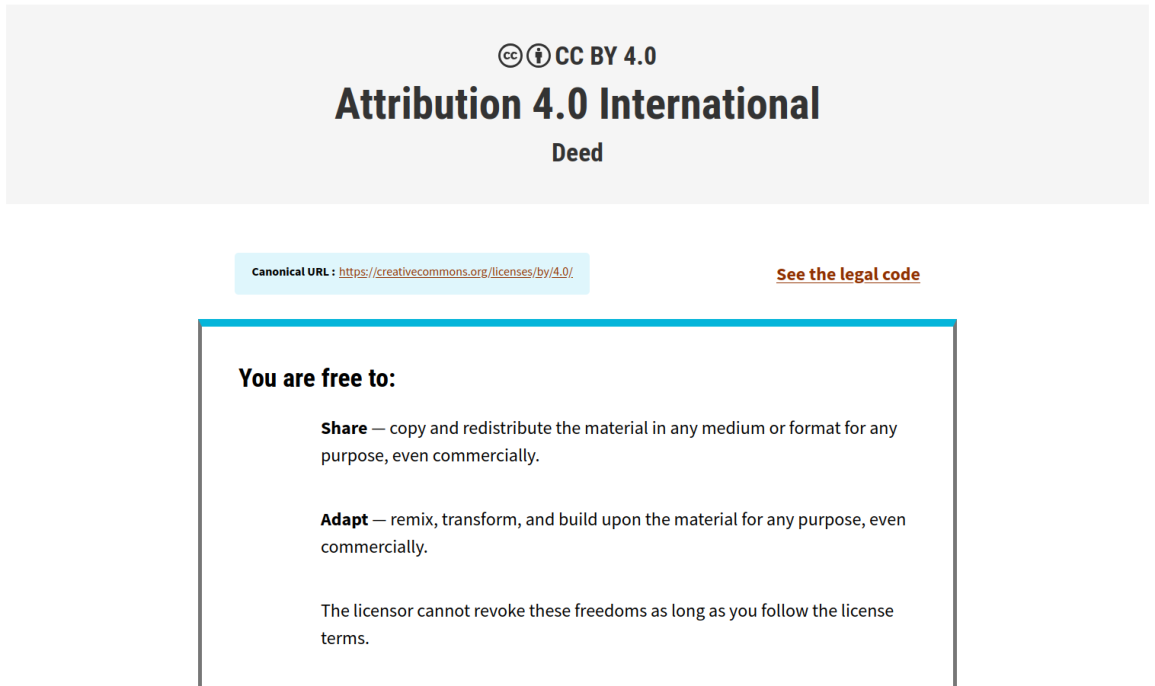
\includegraphics[width=1\textwidth]{FigCC/cc40}}
\caption[Rights to reprint open-access material]{Material that has been previously published under a CC-BY 4.0 license can be reprinted when appropriate credit is given.}
\label{fig:cc40}
\end{figure}

Chapters 2 was published under a CC-BY 4.0 license at the time of preparation of this dissertation. This license allows the reprinting of any previously published material for non-commercial use. Law regarding this license can be read here: \url{https://creativecommons.org/licenses/by/4.0/legalcode.en}
\end{document}                          %% have more than one.
\end{document}
%%%%%%%%%%%%%%%%%%%%%%%%%%%%%%%%%%%%%%%%%%%%%%%%%%%%%%%%%%%%%%%
